% --------------------------------------------

% AP: I have some compatibility issues with the new style (i.e. \section does not work)
\IfFileExists{emulateapjlegacy.cls}{\documentclass[iop]{emulateapjlegacy}}{\documentclass[iop]{emulateapj}}

\usepackage{amsmath}

\usepackage{comment}

preamble.tex
\slugcomment{To be Submitted.}

\makeatletter
\renewcommand\normalsize{\@setfontsize\normalsize\@xpt{12.5}}
% \renewcommand\normalsize{\@setfontsize\normalsize{10.56}{11.4}}      % 11.5, 12.5
\makeatother

\usepackage{xcolor}
\definecolor{apcolor}{HTML}{b3003b}
\definecolor{dlcolor}{HTML}{FF7F00}
\newcommand{\AP}[1]{({\bf \color{apcolor} AP: #1})}
\newcommand{\DL}[1]{({\bf \color{dlcolor} DL: #1})}
\definecolor{afcolor}{HTML}{b3443c}
\newcommand{\AF}[1]{({\bf \color{afcolor} AF: #1})}
\definecolor{mmcolor}{HTML}{006600}
\newcommand{\MM}[1]{({\bf \color{mmcolor} MM: #1})}


% it can be instead included as
% \graphicspath{{Fig/}}
% so that plots are automatically searched for in the given path
\def\figpath{./Fig}

\citestyle{aa}
\shorttitle{Dynamical Properties of MC in Galaxies at the EoR}
\shortauthors{Leung et al.}

\begin{document}
\title{Dynamical Properties of Molecular Cloud Complexes in Galaxies at the Epoch of Reionization}

\author{T. K. Daisy Leung\altaffilmark{1,2}}
\author{Andrea Pallottini\altaffilmark{3,4}}
\author{Andrea Ferrara\altaffilmark{4,5}}
\author{Mordecai-Mark Mac Low\altaffilmark{2,6}}

\affil{\textsuperscript{1} Department of Astronomy, Space Sciences Building, Cornell University, Ithaca, NY 14853, USA; }
\email{tleung@astro.cornell.edu}
\altaffiltext{2}{Center for Computational Astrophysics, Flatiron Institute, 162 Fifth Avenue, New York, NY 10010, USA}
\altaffiltext{3}{Centro Fermi, Museo Storico della Fisica e Centro Studi e Ricerche ``Enrico Fermi'', Piazza del Viminale 1, Roma, 00184, Italy}
\altaffiltext{4}{Scuola Normale Superiore, Piazza dei Cavalieri 7, I-56126 Pisa, Italy}
\altaffiltext{5}{Kavli Institute for the Physics and Mathematics of the Universe (WPI), University of Tokyo, Kashiwa 277-8583, Japan}
%mm \altaffiltext{6}{Institut f{\"u}r Theoretische Astrophysik, Zentrum f{\"u}r Astronomie der Universit{\"a}t Heidelberg, 69120 Heidelberg, Germany}
\altaffiltext{6}{American Museum of Natural History, 79th St.~at Central Park West, New York, NY 10024, USA}

\begin{abstract}
%mm rearranged sentence
We study the properties of molecular cloud complexes (MCs) in a cosmological zoom-in simulation of a
prototypical galaxy (``\flower'') at redshift $z\approx 6$.
%
We identify MCs using an H$_2$ density-based clump finder, and compare their mass, size, velocity dispersion, gas surface density, and virial parameter ($\alpha_{\rm vir}$) with those observed in nearby and \z$\lesssim 2$ galaxies.
%
In \flower, MC masses are in the range $10^{5.5-8.5}$\,\Msun, and have sizes $R\lesssim200$\,pc. Their velocity dispersion and gas surface density are systematically higher than those observed in nearby galaxies, but comparable to starburst galaxies.
%
We identify gravitationally unstable MCs both via an effective, two-component Toomre $Q_{\rm eff}$ parameter 
%mm (gas+stars), 
    taking into account both gas and stars, 
and by using a more observationally accessible $\alpha_{\rm vir}$ analysis. We find that MCs in the main disk of \flower are globally stable, but their internal substructures have low $\alpha_{\rm vir}$ and $Q_{\rm eff}$ values, indicative of
%mm
    instability to gravitational 
collapse.
%
%Our results suggest that the more massive and bigger MCs compared to the Milky Way manifest from the
%higher gas mass fraction, surface density, and velocity dispersion.
% , which together sets the scale for fragmentation.
\AF{Abstract is a bit thin. Revise at the end}
High resolution imaging of the first galaxies with the Atacama Large (sub-)Millimeter Array (ALMA) and the Next Generation Very Large Array (ngVLA) can furnish 
%mm scrutinizing 
data to test our findings and shed light on \SF since the cosmic dark ages.
\end{abstract}
\keywords{methods: data analysis --
          galaxies: high-redshift --
          galaxies: ISM --
          galaxies: evolution --
          galaxies: formation --
          galaxies: starburst --
          stars: formation}

%--------------------------------------------------------------------------
%                                Introduction
%--------------------------------------------------------------------------

\section{Introduction}
The growth of galaxies and their subsequent evolution are governed by the baryon cycle---galaxies accrete gas from the intergalactic medium (IGM) 
%mm to fuel \SF (and feed their  [using "to" implies purpose]
     either directly from the cosmic web, or through mergers with other galaxies.  This gas fuels \SF and feeds central
supermassive black holes. Subsequent feedback replenishes and enriches the circumgalactic medium 
%mm with 
   by expelling some
part of this material. 
%mm [now redundant with first sentence] The general consensus is that the growth of \highz galaxies are triggered and supported by massive gas inflows from mergers and/or the cosmic web at early cosmic times. Back then, 
    Early
galaxies 
%mm themselves 
are more gas-rich and their molecular fraction possibly higher 
%mm compared to
   than
present-day galaxies.

Such massive gas inflows trigger gravitational instabilities that lead to the formation of molecular 
%mm complexes [first use of this term; did you want "cloud complexes" instead of "complexes" for agreement with abstract?] 
   cloud complexes (MCCs)  \MM{changed MC to MCC throughout}
that are typically more massive ($M_{\rm cl}\approx 10^9$\,\Msun) and extended ($\approx$ sub-kpc) than those observed in nearby galaxies (e.g., \citealt{Gabor13a, Hopkins14a, Inoue16a}).
%
Some theoretical works argue that the migration of such giant massive clumps are largely responsible for the buildup of the bulges of massive galaxies at redshift \z$\sim$\,0 \citep[e.g.,][]{Ceverino10a}.

%mm rearranged and combined this and the following paragraph to proceed from observation to conclusion
Early galaxies have higher star formation rates \citep[SFR; ][]{Behroozi13b, Sparre15a, Maiolino15a, Dunlop17a} and smaller sizes \citep[e.g.,][]{Bouwens11a, Ono13a} compared to the local population. 
%
As a consequence, we expect them to be significantly more ionized, and have intense and hard interstelar radiation fields (ISRF). Since their metallicity and dust content are also expected to be lower in these early evolutionary stages, shielding of UV photons---responsible for the photoheating of the gas---  is strongly reduced. Such differences in turn affect the regulation of the thermal and chemical state of the multi-phase interstellar medium (ISM). Studying ISM properties of early galaxies is essential for understanding how \SF proceeds under more extreme conditions.
%
Even in the local Universe, where detailed \obs can be made, variations in 
%mm cloud
     MCC  \MM{do Hughes et al. study cloud complexes, as you do, or can you derive info about complexes from their data?}
properties have been observed between different galaxy populations (see e.g., \citealt{Hughes10a, Hughes13b}).  Given that \highz galaxies statistically represent the early evolutionary stages of present-day galaxies, it is thus reasonable to pose the question: {\it what are the physical properties of MCCs in early galaxies, and how do they differ from those found in local \galpop?}
%

FIR fine-structure lines (e.g., \cii, \nii, and \oiii), and CO and [\ci]~lines are key diagnostics for constraining the ISM conditions of galaxies. They also provide highly complementary information on different ISM phases (ionized, atomic, molecular; e.g., \citealt{Scoville74a, Rubin85a, Malhotra01a}).
%
Global measurements of these diagnostics in \highz galaxies have provided preliminary information on their global properties (e.g., gas masses, gas temperature, and radiation field intensity). However, spatially resolving their ISM is necessary to fully understand many aspects of galaxy evolution and the physics behind their intense \SF (SFR\ssim100$-$3000\,\Msun\,yr\pmOne).
%
To date, spatially resolved ISM properties of \highz galaxies have only been mapped in a handful of (strongly-lensed) galaxies at intermediate-$z$, using tracers such as dust continuum, CO, and \cii lines (e.g., \citealt{Swinbank11a, Hodge15a, Ferkinhoff15a, Hodge16a, Leung19a}). These studies find that galaxies close to the peak of cosmic \SF ($z$\ssim2), are more molecular gas-rich, turbulent, and clumpy than nearby galaxies.

Earlier epochs still represent an essentially uncharted territory for ISM investigations. At present, it remains unclear how \SF proceeds in the (sub-)$L^*$ galaxy population at \z$\gtrsim$\,6  which is responsible for producing the bulk of the UV photons that reionized the Universe.
%
While ALMA has enabled the detection of \cii158\,$\micron$ and CO line emission in normal (SFR$<$\,100\,\Msun\,yr\pmOne) galaxies at \z$>$\,6 over the past few years \citep[e.g.,][]{Carniani18b, Odorico18a}, the first spatially resolved observations are just starting to become available \citep{Jones17a,Smit18a}. 

%mm To answer these questions, isolate key issues, and  accompany ongoing/future experimental efforts, 
    To understand the physical properties of MCCs in early galaxies,
we have undertaken a detailed numerical study whose aim is to characterize the dynamical properties of the star-forming %mm molecular cloud complexes
    MCCs
in prototypical (i.e., $L^*$) galaxies in the Epoch of Reionization (EoR). 

The paper is structured as follows\footnote{Throughout this paper, we adopt a concordance cosmology, with total matter, vacuum and baryonic densities in units of the critical density $\Omega_{\Lambda}$\eq0.692, $\Omega_m$\eq0.308, $\Omega_b$\eq0.0481, Hubble constant $H_0$\eq100\,$h$\,km s\pmOne\,Mpc\pmOne with $h$\eq0.678, spectral index $n$\eq0.967 and $\sigma_8$\eq0.826 \citep{Planck14a}.}. We start by providing some physical background in \Sec{Back}. In \Sec{sim}, we describe the setup of our simulation and properties of our main galaxy (\flower). In \Sec{eqn}, we describe the method used to identify 
%mm molecular gas complexes 
    MCCs,
and present the formalism within which we interpret the results. In \Sec{results}, we present the results and the scaling relations for the MCCs. We then interpret the results and discuss the implications of our findings in \Sec{diss}, and give our conclusions in \Sec{conclusion}.
%
\section{Physical Background}\label{sec:Back}
We begin by introducing some basic material concerning notable physical ("Larson") relations characterizing MCCs, and the gravitational instability of galactic disks, which might be driving MCC formation. Such notions will be used in the subsequent analysis of our simulations. 
\subsection{Larson relations and virial parameter}\label{sec:PVE}
\citet{Larson81a} discussed a number of relations among Galactic 
%mm MCC 
     molecular cloud 
properties, namely the linewidth-size, density-size, and mass-size relations. Larson relations are routinely used for comparing properties of molecular structures in different galactic environments. They also represent a useful framework to analyze our results as they 
%mm
     have been argued to 
arise from the interplay between gravity and turbulence encoded in the virial theorem
%mm 
    (however, note the alternative interpretation involving gravitational collapse by 
    \citealt{Ballesteros-Paredes11}).

%mm In general, the virial theorem for a gas distribution of gas can be written as
     The virial theorem for a distribution of unmagnetized gas can be written as \citep{McKee1992}
\begin{equation}\label{eqn:virial_th_general}
\frac{1}{2}\ddot{\mathcal{I}} = 2(\mathcal{T} - \mathcal{T}_{\rm ext}) + \mathcal{W},
\end{equation}
where $\ddot{\mathcal{I}}$ is the second time derivative of the Lagrangian moment of inertia, $\mathcal{T}$ is the internal energy of the gas, $\mathcal{T}_{\rm ext}$ is external pressure support, and $\mathcal{W}$ is the gravitational energy.
%
Let us specialize to the case of a spherical self-gravitating molecular cloud of mass $M_{\rm cl}$, radius $R$, and root-mean-square velocity dispersion $\sigma$, accounting for both thermal and turbulent contributions. 
%mm Neglecting magnetic field and 
Defining $P_{\rm ext}$ as the external pressure, \Eq{virial_th_general} can be written as
\begin{equation}
\frac{1}{2}{\ddot{\mathcal{I}}} = 3 M_{\rm cl} \sigma^2 - 4\pi P_{\rm ext} R^3 - \Gamma\frac{GM_{\rm cl}^2}{R}\,,
\label{eqn:virial}
\end{equation}
where $\Gamma$ is a geometrical factor that is equal to 3/5 for a uniform sphere; in \Eq{virial} the terms on the right-hand side represent the
%mm  kinetic, external, and gravity pressure terms. 
    kinetic energy, external pressure, and gravitational potential energy terms.

Motivated by Larson's linewidth-size relation \citep{Larson81a} and the work by \citet{Heyer09a}, we assume equilibrium (i.e.\ ${\ddot{\mathcal{I}}}=0$), define the cloud surface density as
$\Sigma$\eq$M/\pi R^2$, and rewrite the previous equation as 
\begin{equation}
\frac{\sigma^2}{R} = \frac{1}{3}\left(\frac{4P_{\rm ext}}{\Sigma} + \frac{3}{5} \pi G \Sigma \right)\,,
\label{eqn:v0}
\end{equation}
which further reduces to 
\begin{equation}
\frac{\sigma^2}{R} = \frac{\pi}{5} G \Sigma\,,
\label{eqn:SVE}
\end{equation}
if the external pressure $P_{\rm ext}=0$. For this case (often referred to as simple virial equilibrium) from the balance between kinetic and gravity terms we can define the virial parameter as 
\begin{equation}
\alpha_{\rm vir} \equiv  \frac{5\sigma^2R}{GM_{\rm cl}} = \frac{5\sigma^2}{\pi G \Sigma R}\,,
\label{eqn:alpha}
\end{equation}

Based on Equation~\ref{eqn:SVE}, a one-to-one mapping between $\sigma^2/R$ and $\Sigma$ is therefore expected for a virialized cloud, since $\sigma^2/R\propto\Sigma$. Deviations from this relation are usually attributed to a significant contribution from external pressure as per Equation~\ref{eqn:v0} (see e.g., \citealt{Heyer09a, Hughes10a, Hughes13b, Meidt13a}).

Summarizing, the virial parameter can be used to quantify the stability/boundedness of 
%mm an MCC. 
    a molecular cloud.
Accounting for the external pressure, a virial parameter of $\alpha_{\rm vir}\lesssim2$ would be unstable \citep{bertoldi:1992}.
%
Such a criterion\footnote{In the following, to facilitate comparison with \obs, we derive $\alpha_{\rm vir}$ using the gas component only and ignore contributions due to the stellar component.} is often used in \obs \citep[see e.g., ][]{Kauffmann17b}. 

%\subsection{Gravitational Instabilities}\label{sec:Q}
\subsection{Toomre stability analysis}\label{sec:Q}

The onset of gravitational instability is 
%mm considered to be 
tightly connected to \SF \citep[e.g.,][]{Kennicutt89a, Wang94a, Li05b, Li06a}. 
%mm [rearranged to put derivation before result]
For axisymmetric modes, the dispersion relation for the growth of density perturbations in a rotating, turbulent disk of finite thickness $h$ is described by
\begin{equation}
\omega^2 = \kappa^2 - \frac{2\pi G \Sigma |k|}{1 + |k| h} + \sigma_{\rm disk}^2 k^2\,,
\label{eqn:3Ddisp}
\end{equation}
where $k$ is the wavenumber and $\kappa$ is the epicyclic frequency, defined as:
\begin{equation}
\kappa^2\equiv\frac{2\Omega}{\altomega}\frac{d}{d\altomega}\left(\altomega^2\Omega\right)\,.
\label{eqn:kappa}
\end{equation}
\citep{Romeo92a}.
\AF{$R$ is not the same as the MCC radius in the prev.\ Section} \MM{replaced $R$ with $\altomega$, and $\sigma$ with $\sigma_{\rm disk}$.}
In Equation~\ref{eqn:3Ddisp} the terms on the right hand side are related to rotation, self-gravity and internal pressure, respectively. 
%mm
    Heuristically, the instability can be understood by considering the scale
 at which gravitational potential overcomes the internal energy. Gravity dominates at scales $L > L_J$, where $L_J$ is the Jeans length. However, 
%mm centrifugal forces resulting from
   shearing by 
differential rotation in disk galaxies can stabilize perturbations 
%mm even on these scales. 
    that might otherwise collapse for $L > L_{\rm rot}$, where $L_{\rm rot}$ is set by $\kappa$.
%mm As a result, a disk is thought to be unstable on
    As a result, disks are unstable to gravitational collapse on 
scales between $L_J < L < L_{\rm rot}$.  

From the dispersion relation, a parameter $Q$ can be derived such that $Q < 1$ when instability occurs, that reproduces this inequality to order unity.
For a collisionless fluid---such as an ensemble of stars--- this parameter is \citep{Toomre64a}
\begin{equation}
Q_{\star} \equiv\frac{\sigma_{\star}\kappa}{3.36 G \Sigma_{\star}}\,.
\end{equation}
The equivalent parameter for a collisional gas was derived by
%mm [corrected from Toomre64a to Goldreich65a (not Goldreich65b, which is about spiral arm formation)]
    \citep{Goldreich65a}:
\begin{equation}
Q_{\rm gas}\equiv\frac{\sigma_{\rm gas}\kappa}{\pi G \Sigma_{\rm gas}}\,.
\label{eqn:Q}
\end{equation}
In the thin disk approximation ($kh\ll1$), instability ($\omega^2 < 0$ in  \Eq{3Ddisp}) occurs on scales $k$ such that $Q < Q_{\rm crit}\simeq1$ (or equivalently $\omega^2 < 0$). 
%mm  In theoretical and observational works, gravitational instability has been widely discussed in the context of the Toomre $Q$ stability criterion \citep{Toomre64a, Goldreich65b} or its observable proxy
     A frequently used observable proxy for $Q$ is the ratio of disk circular velocity to root-mean-square velocity dispersion
$v_{\rm circ}/\sigma_{\rm disk}$
%mm , i.e., the circular velocity to the disk r.m.s. velocity dispersion \AF{This is not exactly the same $\sigma$ as before} \MM{see above} ratio 
\citep[e.g.,][]{GarciaBurillo03a, Genzel11a, Kassin12a, Leung19a}.
% https://ned.ipac.caltech.edu/level5/March15/Glazebrook/Glazebrook5.html
%
% from linear analysis

In our stability analysis, we account for the combined effect of gas and stars 
%mm 
     \citep[derived exactly by][]{Rafikov01}, 
and for the non-negligible disk thickness. This is done by adopting an approximation for an effective two-component $Q_{\rm eff}$ parameter \citep[i.e.,][see also \citealt{Inoue16a}]{Romeo11a}.
%
The effect of disk thickness modifies the $Q$ parameter for gas and stars by accounting for the vertical velocity dispersion:
\begin{equation}
T_{x} = \left\{
		\begin{array}{lccr}
			{\displaystyle 0.8 + 0.7\left(\frac{\sigma_{z}}{\sigma_{r}}\right)}      && & \mbox{if\ } \sigma_z \lesssim 0.5 \times \sigma_r \\ [1.25em]
			{\displaystyle 1 + 0.6\left(\frac{\sigma_{z}}{\sigma_{r}}\right)}        & & & \mbox{if\ } \sigma_z \gtrsim 0.5 \times \sigma_r
\\
		\end{array}
	\right.
\end{equation}
and
\begin{equation}
Q^{\rm thick}_{x} = T_{x} Q\,,
\end{equation}
with $x$ indicating either gas or stars.
% Note that w/ thickness, there's the a self-gravity dilution term in the dispersion relation, which in effect reduceds the surface gravity in the vertical direction. As such, it is easier to be stable against gravitaional instability. Thus, the criterion for instability $Q$ is reduced.
%
The combined effect of gas and stars can then be accounted for by writing
\begin{equation}\label{eqn:q_eff}
Q^{-1}_{\rm eff} =  \left\{
				\begin{array}{lccr}
					     {\displaystyle\frac{w}{Q^{\rm thick}_{\star}} + \frac{1}{Q^{\rm thick}_{\rm gas}}}      & & & \mbox{if\ }  Q^{\rm thick}_{\star} \geq Q^{\rm thick}_{\rm gas} \\ [0.75em]
                                               {\displaystyle\frac{1}{Q^{\rm thick}_{\star}} + \frac{w}{Q^{\rm thick}_{\rm gas}}}      & & & \mbox{if\ } Q^{\rm thick}_{\star} \leq Q^{\rm thick}_{\rm gas} \\
				\end{array}
			    \right.
\end{equation}
where the relative weight $w$ is defined as:
\begin{equation}
w\equiv\frac{2 \sigma_{\star} \sigma_{\rm gas}}{\sigma_{\star}^2 + \sigma_{\rm gas}^2},
\end{equation}
Conceptually, the finite disk thickness reduces the gravity in the vertical direction, thereby making it easier for a system to
%mm obtain
    maintain 
stability, and thus lowering the critical Toomre $Q_{\rm crit}$ from $\simeq$\,1 to 
0.67 \citep{Goldreich65a}.
%
On the other hand, including the contribution of the stellar component promotes gravitational instability, and thus increases
%mm  the criterion of the Toomre
$Q_{\rm crit}$, 
%mm, unless it is dynamically hot to ``compensate''. 
   moreso if the stars have low velocity dispersion.
As a rule of thumb, $Q_{\rm crit}\eq1.34$ for $Q_{\rm gas}$\eq$Q_\star$.  % 0.67 * 2

% ------------------
\section{Numerical simulations}\label{sec:sim}
The simulations used in this work are described by \citealt{Pallottini17a, Pallottini17b} and are only briefly summarized here.
%
\ncode{Serra}\footnote{Greenhouse in Italian} is a suite of cosmological zoom-in simulations performed using Eulerian hydrodynamics and adaptive mesh refinement (AMR) techniques to achieve high spatial resolution in regions of interest (e.g., regions of high density).
%
In particular, it uses a modified version of \ncode{ramses} \citep{Teyssier02a} as the AMR backend. The simulation used here covers a comoving box of 20\,Mpc $h$\pmOne in size, 
%mm resolving down to a physical scale of 
     with the finest refined cell sizes 
$l_{\rm cell}\approx$\,30\,pc (at $z\sim6$) and a (baryonic) mass resolution
%mm
    \MM{Is this really the resolution of dark matter particles?  The baryonic mass (i.e.\ gas) resolution depends on the 
    local density, which would have to be specified here.}
 of $m_b\simeq$\,10$^4$\,\Msun at the finest level. 
%mm Such a physical scales are comparable to those of
     Cell sizes are comparable to the sizes of
local giant molecular clouds \citep[e.g.,][]{Sanders85a, Federrath13a, Goodman14a},
%mm 
     \MM{Nota Bene!} although the resolved scale of 5--10 cells is rather larger.

%mm We
    The models 
include a chemical network 
%mm including ${\rm e}^{-}, \rm{H}$, $\rm{H}^{+}$, $\rm{H}^{-}$, $\rm{He}$, $\rm{He}^{+}$, $\rm{He}^{++}$, $\rm{H}_2$, $\rm{H}_2^{+}$ 
   following e$^{-}$, H$^+$, H$^-$, He, He$^+$, He$^{++}$, H$_2$, and H$_2^+$
\citep{Grassi14a,Bovino16a}. Of particular importance here is that abundances are calculated using an on-the-fly non-equilibrium formation of molecular hydrogen scheme 
%mm following \citet{Pallotini17b} [the order had to be reversed for alphabetization]
    described by \citet{Pallottini17a}.

% radiative feedback --> NT pressure
Star formation is modeled using an H$_2$-based prescription of the Schmidt-Kennicutt relation \citep{Krumholz09a}. We adopt stellar tracks from \ncode{starburst99} and include stellar feedback from supernovae (SNe) 
%mm and OB/AGB stars. 
   as well as OB and asymptotic giant branch stars.
Coupling to the gas is implemented via a sub-grid model for blastwaves, which accounts for radiative energy losses inside the cell. The remaining energy is injected into the ISM in kinetic and thermal energy forms. Radiation pressure on dust and gas is also included (see \citealt{Pallottini17a} for details).  
%mm
   \MM{confirm:} Photoionization and stellar wind feedback is neglected.

The simulation zooms in on a galaxy named
%mm 
   after the flower 
\flower whose properties are given in 
%mm \citet{Pallottini17b} 
      \citet{Pallottini17a} 
and are briefly summarized in the following. \flower is a Lyman-break galaxy 
%mm (LBG), [unused acronym]
that at $z\simeq 6$ is hosted by a dark matter halo of mass $M_{\rm DM}\simeq$\,10$^{11}$\,\Msun at the center of a cosmic web knot, and accretes mass from the IGM mainly via three filaments of length $\simeq$\,100\,kpc. \flower has a stellar mass of $M_\star\simeq$\,3\E{10}\,\Msun, a metallicity of $Z\simeq$\,0.5\,$Z_{\odot}$, a molecular gas mass of $M_{\rm H2}\simeq$\,5\E{7}\,\Msun, and a SFR of $\simeq$\,100\,\Msun\,yr\pmOne. \MM{What is its gas fraction?  I ask because its molecular gas mass is minuscule, particularly for such a high SFR: this is a depletion time of only 0.5 Myr, while modern galaxies usually have depletion times more like 0.5--2~Gyr!} Its effective stellar radius  is $\sim$0.5\,kpc and the dark matter virial radius is $r_{\rm 200}\simeq$\,15\,kpc.

\subsection{Star Formation History} \label{sec:sfh}

\begin{figure*}
\centering
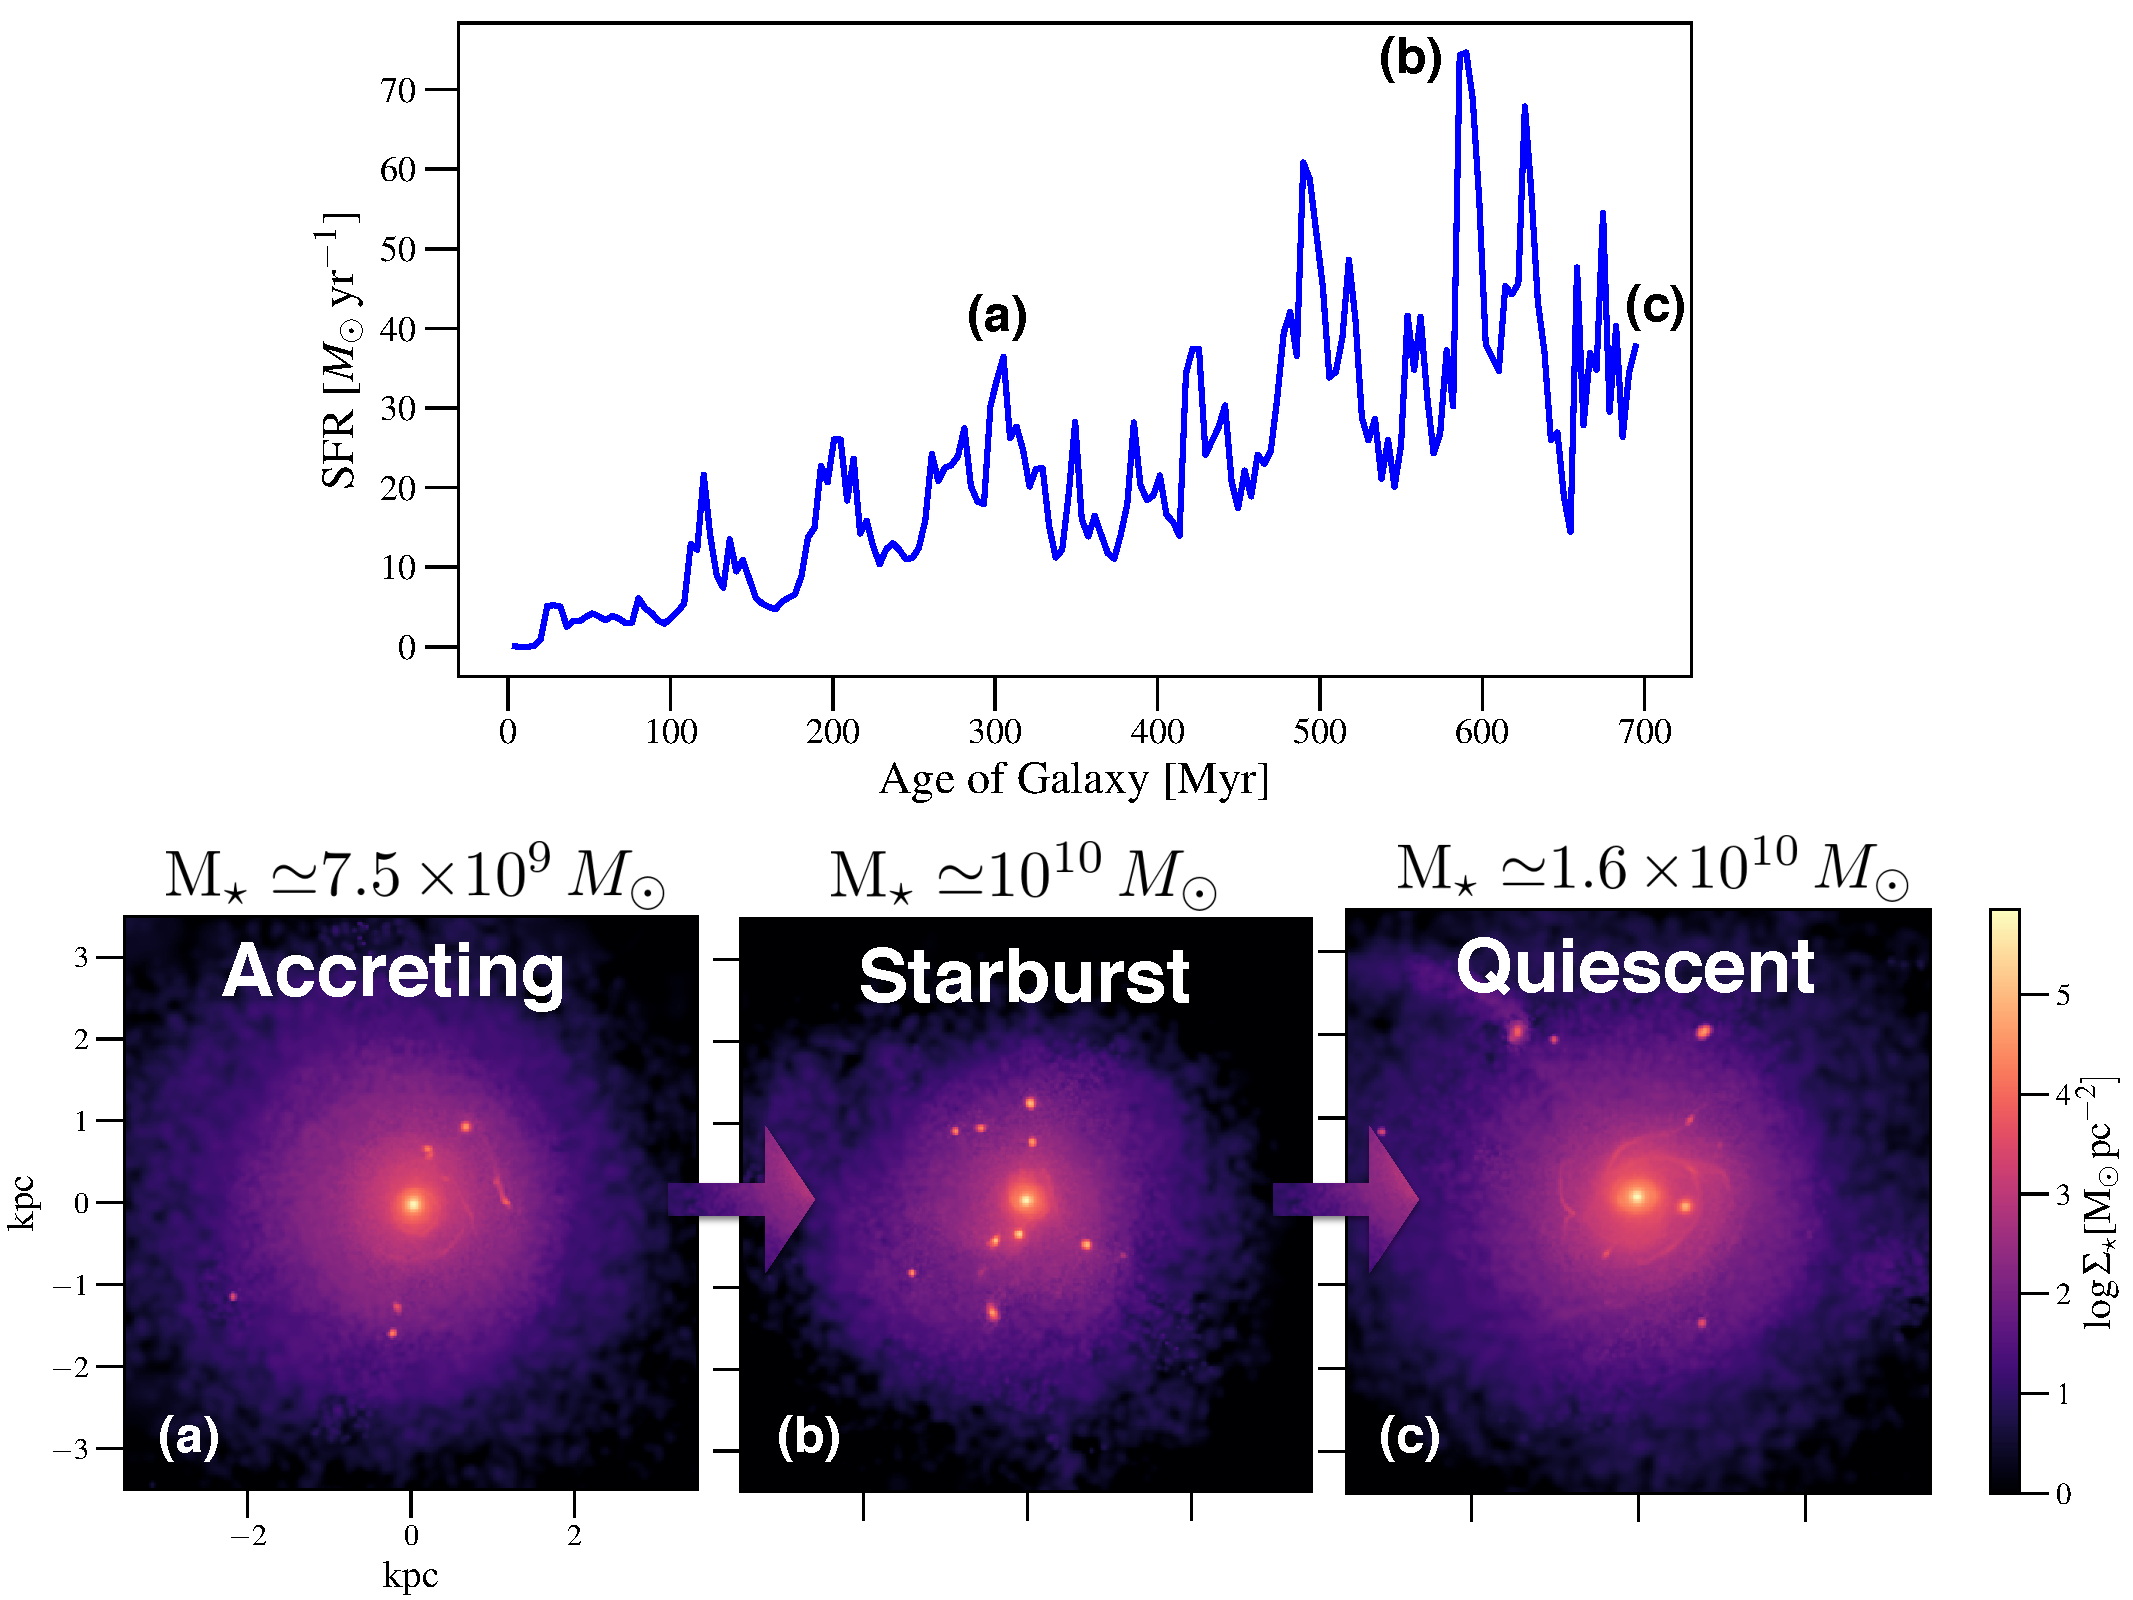
\includegraphics[trim=0 0 0 0, clip, width=0.65\textwidth]{\figpath/sfh.pdf}
\caption{
    {\it Top panel}: Star formation history of \flower. {\it Bottom}: projected stellar mass distribution during {\it (a)} an early accretion phase;  {\it (b)} a major starburst following a merger event; and {\it (c)} a relatively quiescent post-starburst phase.
\label{fig:SFH}}
\end{figure*}

One of the main advantages for studying the dynamical properties of simulated galaies is the fact that we can examine how their properties evolve with time.
%
%This is advantageous especially at early cosmic epochs, when the densest structures are beginning to form; gas is constantly being accreted onto the central galaxy from the cosmic web and satellite galaxies, thereby leading to bursts of \SF. Meanwhile, tidal forces resulting from interactions with these surrounding galaxies can disrupt the main disk and arms, likely leading to different dynamical states for the molecular structures compared to more evolved galaxies found at a later cosmic time (e.g., some molecular structures may disperse while others may agglomerate into more massive ones). % mainly expecting differences in alpha_vir, sigma, M_cl.

The \SF history\footnote{Note that here the SFR is calculated based on the stellar mass formed in the last 10 Myr within 3.5 kpc from the galaxy center of mass. The SFR plotted in Figure 2 of \citet{Pallottini17b} is a factor of two higher since there the SFR account for the contribution from massive satellite galaxies within the virial radius ($\approx$15\,kpc).} of \flower is shown in \Fig{SFH}. The SFR of \flower varies between $\sim$30$-$80\,\Msun\,yr\pmOne as it evolves from an actively accreting phase to a starburst phase after a merger, and then back to a relatively quiescent phase, over the simulated $\approx 700$ Myr.

Given \flower's SF stochastic nature, in this work we mostly focus on the analysis of two of its most extreme evolutionary stages (see \Sec{singless}). The two phases correspond to (a) intense accretion (b) starburst (\Fig{SFH}). We are interesting in determining whether MCC properties are sensitive to these different dynamical conditions. For completeness, for the other evolutionary stages traced in the simulation we only show scaling relations (see \Fig{alpha16-28}).

Throughout this paper, we dub as ``satellite galaxies'' the dense gas regions outside the main disk of \flower. The distinction between clumps and satellites is admittedly somewhat ambiguous, and we consider it only as a working one.
\AF{To be discussed at the end}

\section{Molecular Cloud Complexes}\label{sec:eqn}

\subsection{Identification}\label{sec:method}

To identify the molecular complexes, we use a customized version of the ``clump-finding'' algorithm available in the \ncode{python} package \ncode{yt} \citep{Turk11a}, which was initially described in \citet{Smith09a}, but this function has been modified since then.
%
The latest version of the default \ncode{yt} clump finder decomposes the zones of the simulation into non-overlapping tiles, which are stored in a $k$-dimensional tree ($k$-D tree). It then identifies the contours of a variable field (here, the density field) within a tile and connects them across the tiles. In the customized version used for this study, we modify the function to enhance the stability of the code.
%
Due to the nature of our AMR simulation, we regrid the simulation data into uniform grids. The grid size is defined based on the highest resolution of the simulation data, i.e., the less refined regions are supersampled in the resulting uniform grids.

In the clump-finding process, we employ a set of different density thresholds defined based on the molecular hydrogen density of \flower at different evolutionary stages ($z$\eq6.0\,$-$\,7.2).
%
We note that this process is in essence similar to identifying molecular structures based on the noise levels of surface density maps observers obtain with telescopes, using molecular line tracers such as CO, CS, and HCN, as commonly adopted in observational studies (e.g., identifying clumps based on/after applying S/N-clipping, using tools such as \ncode{aips}'s task \ncode{serch}, \ncode{clumpfind}, and \ncode{cprops}; \citealt{Williams94a, Oka01a, Rosolowsky06a, Rosolowsky08a}).
%
We note that, owing to the nature of \obs, such structures are identified in position-position-velocity (PPV) space, whereas in simulations, one has the full 6D spatial-kinematic information, and can therefore cleanly identify structures directly using the density field in position-position-position (PPP) space.
% Many concerning the correspondence between  ... , dating back to the work by \citep{Adler92a}.
Existing studies find a good correspondence in the dynamical properties extracted in PPV- versus PPP-space (\citealt{Ballesteros-Paredes02a, Heitsch09a, Shetty10a, Beaumont13a, Pan15a}, but see also \citealt{Shetty10a} for a discussion on caveats and limitations).
% large scale structure in PPP may be identified as numerous lower mass structures in the PPV cube due to gradients in the LOS and conversly, superposition when spatially distinct components with the same velocity are "merged" into one component in the PPV space when observed along the LOS (see Fig. 1 of Beaumount13a). (may be worth putting more thoughts on this after the report is due).

\begin{figure}[htbp]
\centering
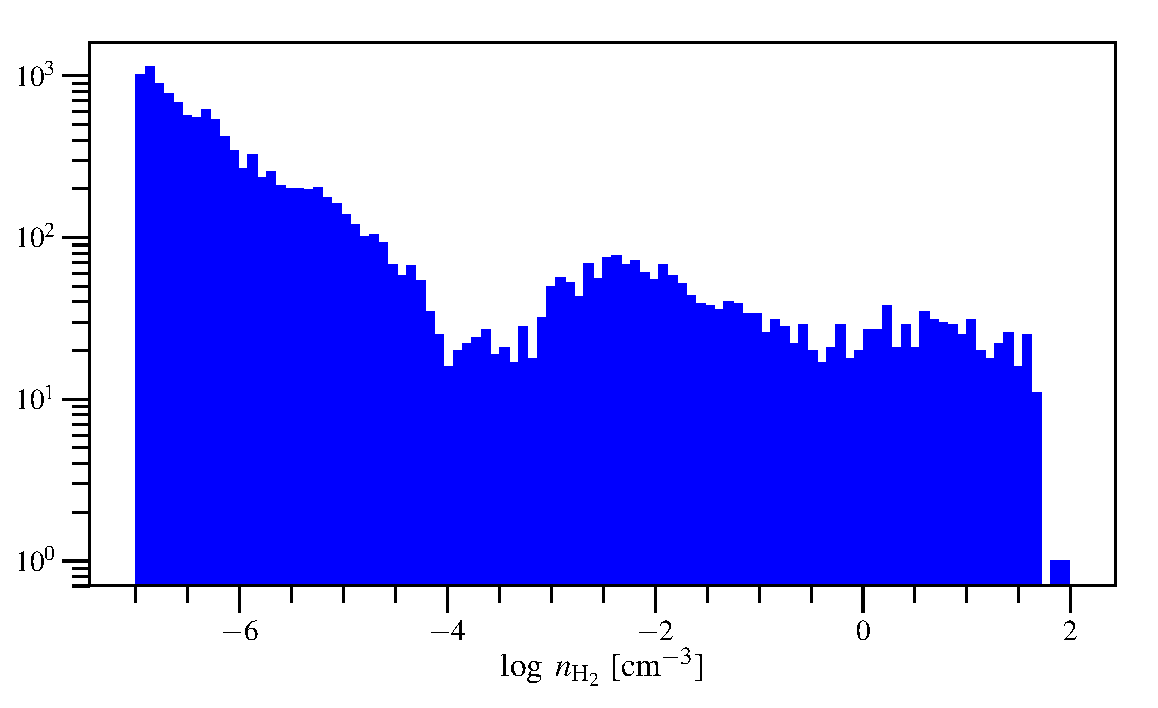
\includegraphics[trim=0 0 0 0, clip, width=0.5\textwidth]{\figpath/hist_test_16.pdf}
\caption{Probability distribution function of the H$_2$ number density in \flower during the accretion phase shown in \Fig{SFH}.
\label{fig:h2density}}
\end{figure}

\begin{figure*}[htbp]
 \centering
  \includegraphics[scale=0.6]{\figpath/{dual_16_ncut_0.53}.pdf}
  \\ [-2.9em]
  \includegraphics[scale=0.6]{\figpath/{dual_16_ncut_6.81}.pdf}
  \\ [-2.9em]
  \includegraphics[scale=0.6]{\figpath/{dual_16_ncut_18.96}.pdf}
\caption{
Examples of MCCs (white contours) identified by the clump-finder in  \flower during its  accreting phase. The color-bar shows the mean H$_2$ number density, weighted by gas mass. Different rows shows the clump-finder results obtained by applying different H$_2$ number density cuts density cuts $(n_{\rm cut})$ as shown by the label. Left and right panels show the galaxy from different viewing angles.
\label{fig:MCC}}
\end{figure*}

In \Fig{h2density}, we show the H$_2$ number density ($n_{\rm H2}$) distribution of \flower~in its accreting phase, by including the contribution from the gas within 3.5 kpc from the galaxy center.
%
We note that the distribution is almost flat for $n_{\rm H2}\gtrsim1$\,\cc and it samples the range of densities where clumps are found based on morphological analysis\footnote{For $n_{\rm H2}\gtrsim1$\,\cc the fourth Minkowsky functional of the H$_{2}$ density field is significantly larger than zero. This implies that the field is made of isolated components. See Fig. 6 in \citet{Pallottini17b}.} \citep{Pallottini17b}. We identify MCCs by applying 10 equally-spaced volumetric H$_2$ density cuts of ${(n_{\rm cut}/{\rm cm^{-3})}}\eq[0.32, 0.53, 0.88, 1.45, 2.45, 4.08, 5.81, 11.36, 18.96, 31.62]$\footnote{We also tested variations in $n_{\rm cut}$ range and found no qualitative differences (see \Sec{ncut}).} to each snapshot.

To visually appreciate  the clump finding procedure, in \Fig{MCC} we overplot the molecular structures identified using a subset of the H$_2$ density cuts ($n_{\rm cut}$\eq0.53, 5.81, and 18.96\,\cc) on the H$_2$ density maps.
Since the molecular structures identified could easily appear as overlapping structures depending on the viewing angle, we also plot them in different three-dimensional projections (right panels of \Fig{MCC}) so that one can more easily see that they are collections of disjoint structures.
%
We repeat this identification process for 14 evolutionary stages between redshift \z$\in$[6.0, 7.2], spaced by $\Delta t$\eq50\,Myr.

Note that we impose the additional constraint that an identified structure must be composed of at least 10 cells. We caution that an important caveat of such constraint is that we can only examine the parameter space of ``cloud'' of typical size $R\gtrsim 60$\,pc, because of the resolution limit in the simulation.

\subsection{Molecular Cloud Properties}

% Molecular clouds are the natal place for \SF, their structure and dynamics hold important clues to understanding
% the mechanisms and physics of formation and evolution of molecular structures and \SF.
Upon identifying the molecular structures, we extract properties such as the gas mass ($M_{\rm cl}$), effective size ($R$), Mach number ($\mathcal{M}$), r.m.s. velocity dispersion ($\sigma$), and gas surface density ($\Sigma_{\rm gas}$) to examine their dynamics.

The mass of an MCC is calculated from the uniformly-gridded 3D density field, integrating over the MCC volume $V$. The effective size is defined assuming spherical geometry, i.e. $R \equiv (3 V /4 \pi)^{1/3}$.
%
The velocity dispersion of MCCs is calculated from non-thermal velocity dispersion ($\sigma_{\rm NT}$) and thermal sound speed ($c_s$):
\begin{equation}
\sigma^2 = \sigma_{\rm NT}^2 + c_s^2.
\label{eqn:veldisp}
\end{equation}
%
In \obs of MCC, the linewidths contribution of dense gas contribution is larger then the one from the diffuse gas. We therefore calculate each term on the RHS of Equation~\ref{eqn:veldisp} as a density-weighted quantity. For instance, the non-thermal velocity dispersion is calculated as follows:
\begin{equation}
\sigma_{\rm NT}^2 = \frac{1}{{3}}\frac{\sum_{i} \rho_i \left|\mathbf{v}_i - \mathbf{\bar v}\right|^2}{\sum_i \rho_i}\,,
\end{equation}
where the sum is done for the cells composing each MCC.
%
The local sound speed of all identified molecular complexes is much smaller than their turbulent velocities\footnote{Velocity dispersions calculated from velocity field are comparable to those calculated from the pressure field, indicating that contribution from shear is unlikely to dominating the velocity dispersions reported here.\label{ftn:veldisp}}. On average, the Mach number of the MCCs is  $\mathcal{M} = \sigma_{\rm NT}/c_s\approx 50$. This is consistent with the global analysis done on \flower by \citet{Vallini18a}.

We show in \Fig{dist} the MCC distribution in terms of their molecular gas mass, radius, and gas mass fraction, which we define as
\begin{equation}
f_{\rm gas} = \frac{M_{\rm cl}} {\left(M_{\rm cl} + M_\star\right)},
\end{equation}
where $M_\star$ is the stellar mass within the MCC volume.
%
We note that the distributions vary for different evolutionary stages of \flower. The highest density threshold of $n_{\rm cut}$\eq31.62\,\cc yields a minimum MCC mass of the order of 10$^{5.5}$\,\Msun for the densest MCC.
%
We find $\sim$10$-$13 MCCs with masses exceeding 10$^8$\,\Msun across all the evolutionary stages considered in this work, for each  $n_{\rm cut}$ value. \AF{This is true only for low $n_{cut}$? Why in Fig. do you show the valu 18.96 instead?} \DL{MCCs w/ Mcl $>$10$^8$\,\Msun is the case for each ncut.} Such massive clouds correspond to the galaxy molecular disk, that is identified as a single component for low $n_{\rm cut}$. The mass of the MCCs identified ranges between $M_{\rm cl}\approx$10$^{5.5-8.5}$\,\Msun, consistent with those observed in \z$\sim$2 galaxies in rest-frame UV and optical light \citep{Elmegreen07a, Elmegreen09a}. \AF{you do not comment on $R$ and $f_{gas}$ here..Also, what is the total number of MCCs?}

\begin{figure*}[htbp]
\centering
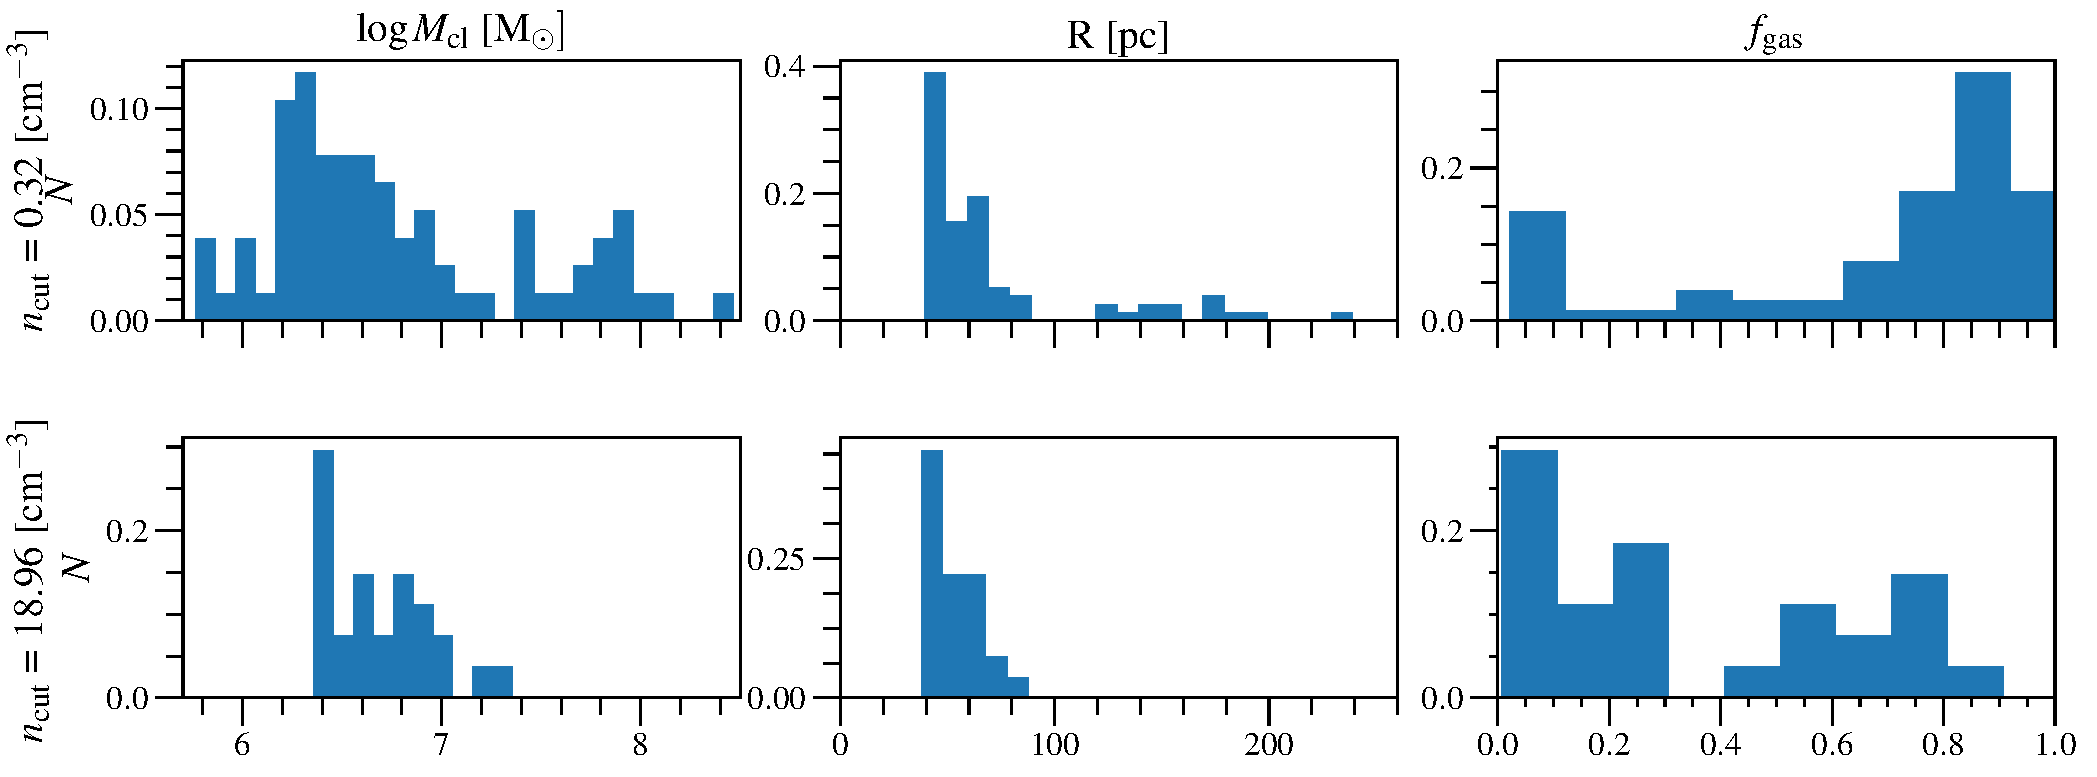
\includegraphics[trim=0 0 0 0, clip, width=\textwidth]{\figpath/minmaxNcut_basicDistributions.pdf}
\caption{Distributions of mass (left), size (middle), and gas mass fraction (right) of MCCs identified using the lowest $n_{\rm cut}$ (top panels) and $n_{\rm ncut}$\eq18.96\,\cc (bottom panels).
Note that the scale shown on the y-axes are different between the top and bottom panels, as less MCCs are identified at higher $n_{\rm cut}$.
\label{fig:dist}}
\end{figure*}


\section{Results}\label{sec:results}

\begin{figure*}
\centering
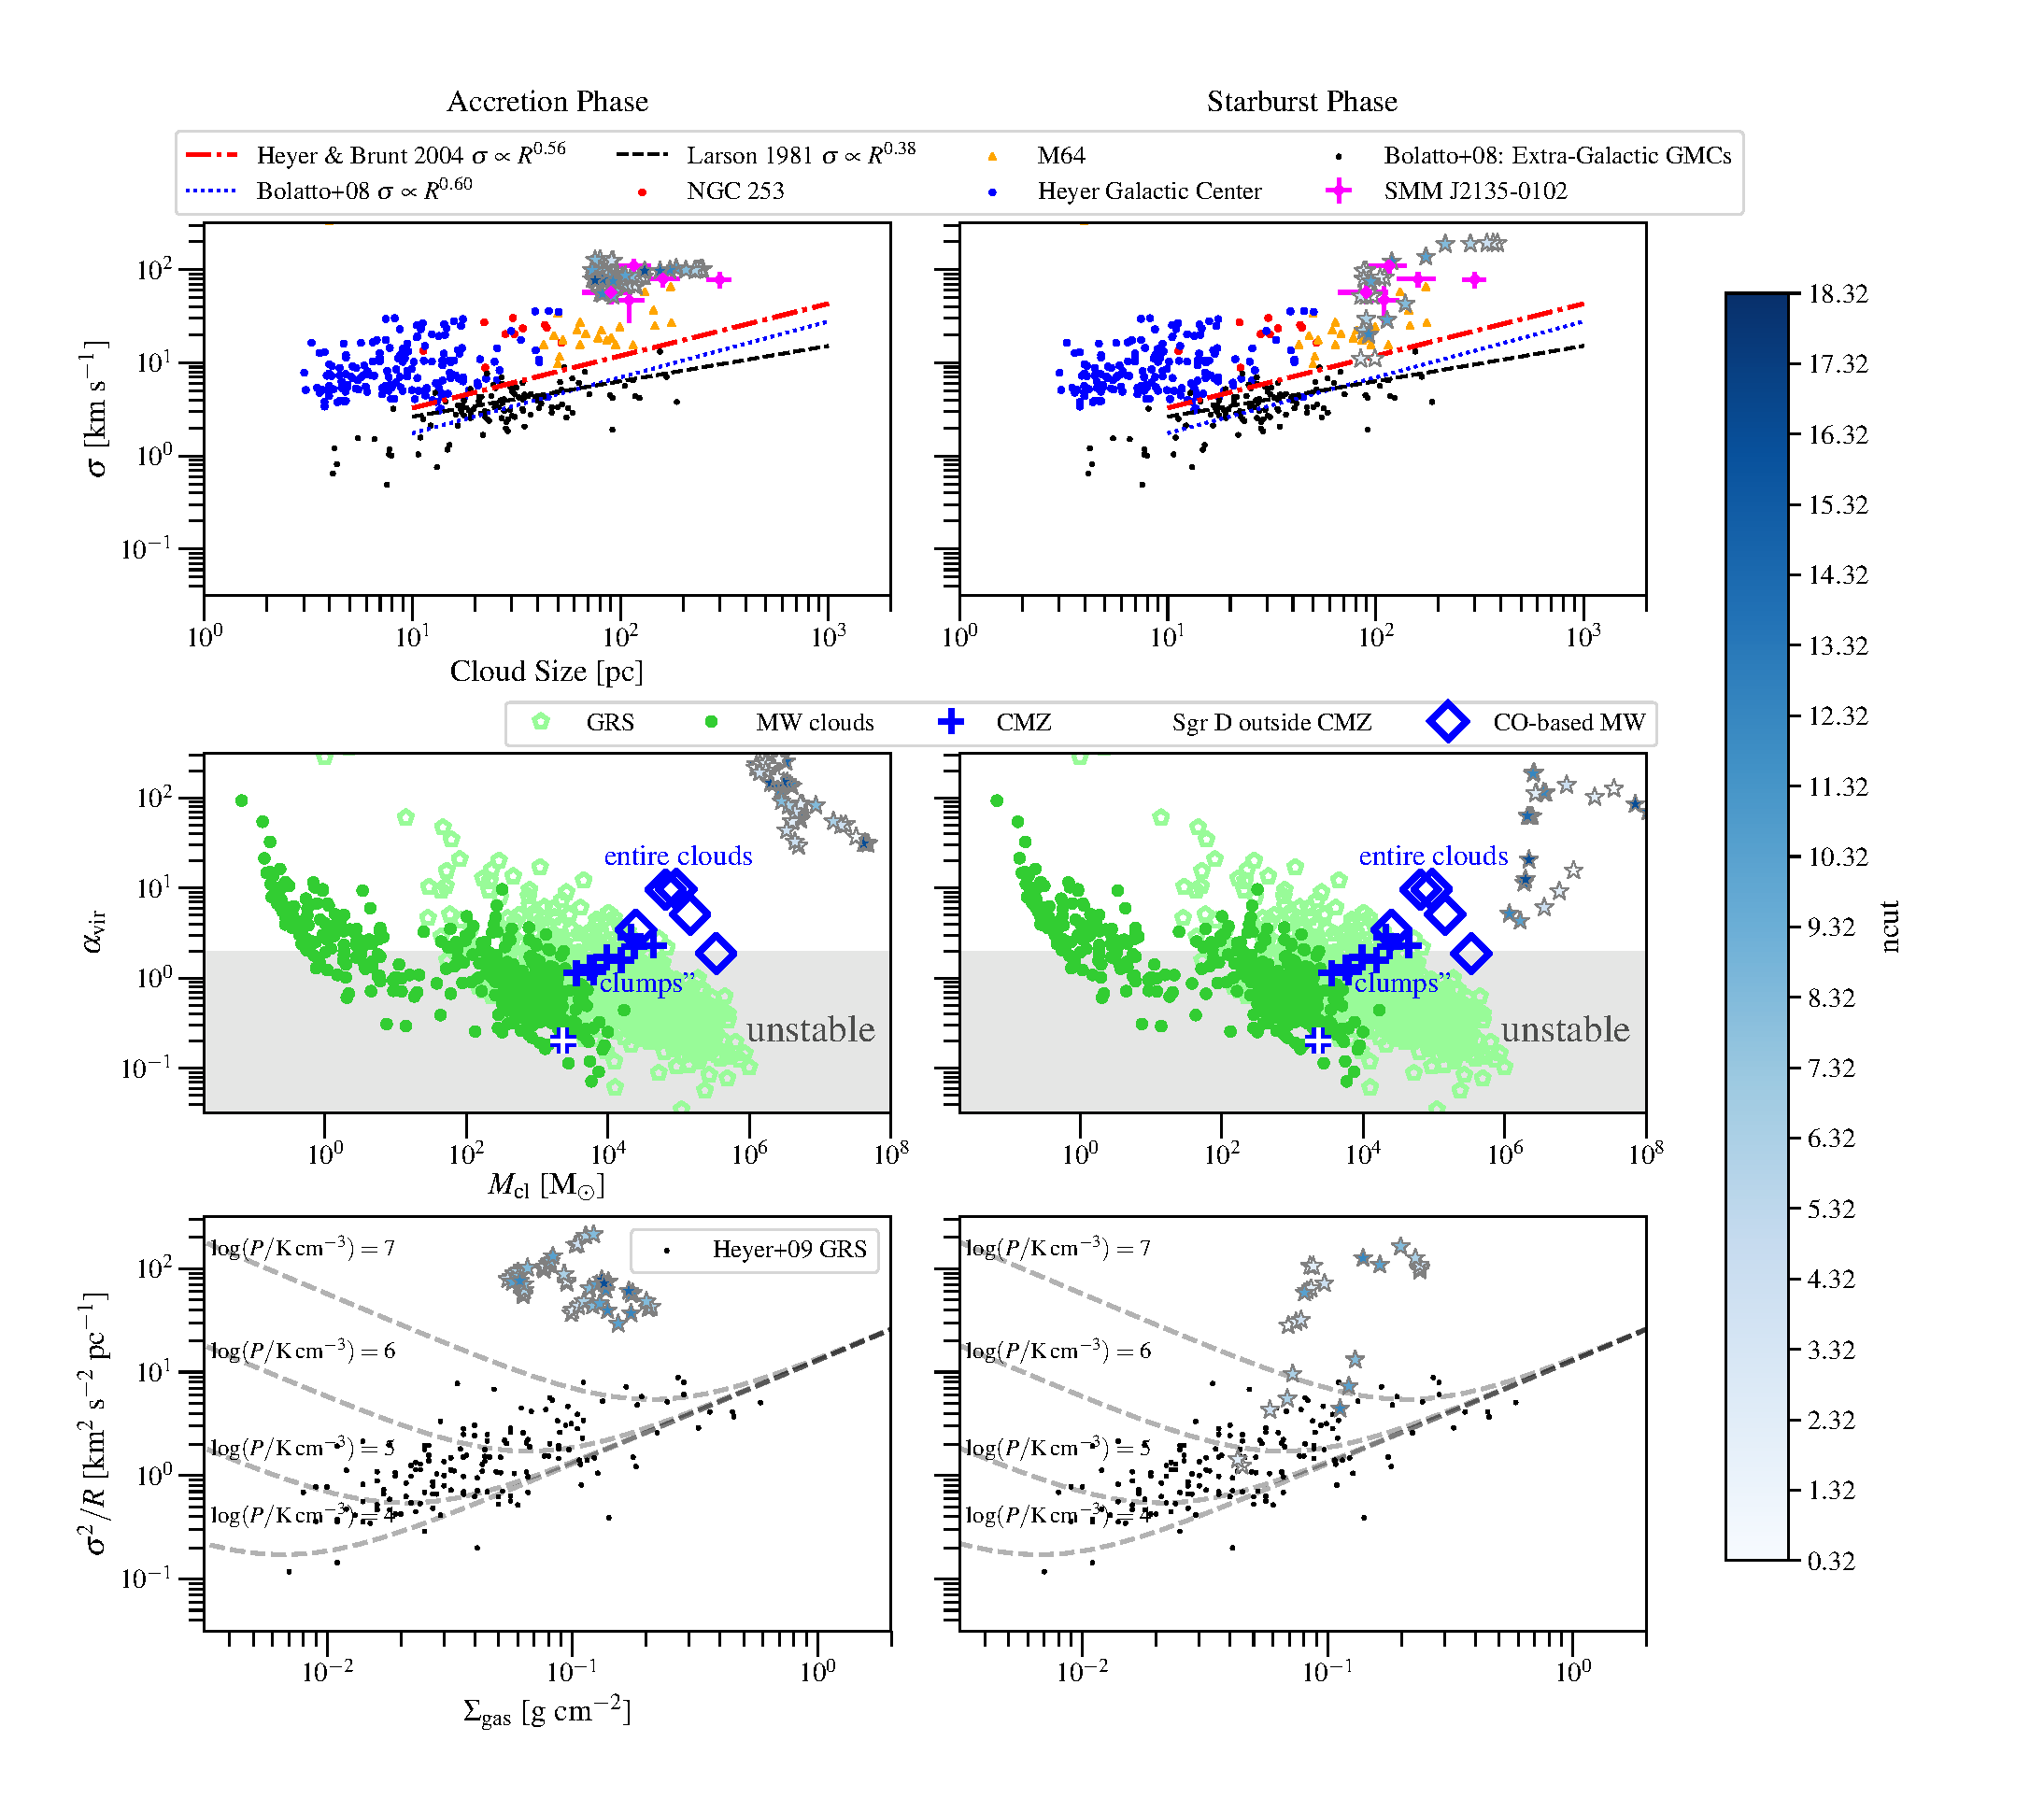
\includegraphics[trim=0 0 0 0, clip, width=1.05\textwidth]{\figpath/3by2_clumpProp_ss16-27.pdf}
\caption{
Linewidth-size relation (top), $\alpha_{\rm vir}$-mass relation (middle), and $\sigma^2/R$-$\Sigma_{\rm gas}$ relation (bottom) for MCCs (star symbols) identified in the two most extreme evolutionary stages of \flower\ --- accreting phase (left) and starburst phase (right). Star symbols are color-coded by the density thresholds ($n_{\rm cut}$). 
Data points in the $\alpha_{\rm vir}$-mass figure are taken from \citet{Kauffmann17a} and \citet{Kauffmann17b} and references therein (see Fig 4 of \citealt{Kauffmann17b}).
\label{fig:larsons_single}}
\end{figure*}

\begin{figure*}
\centering
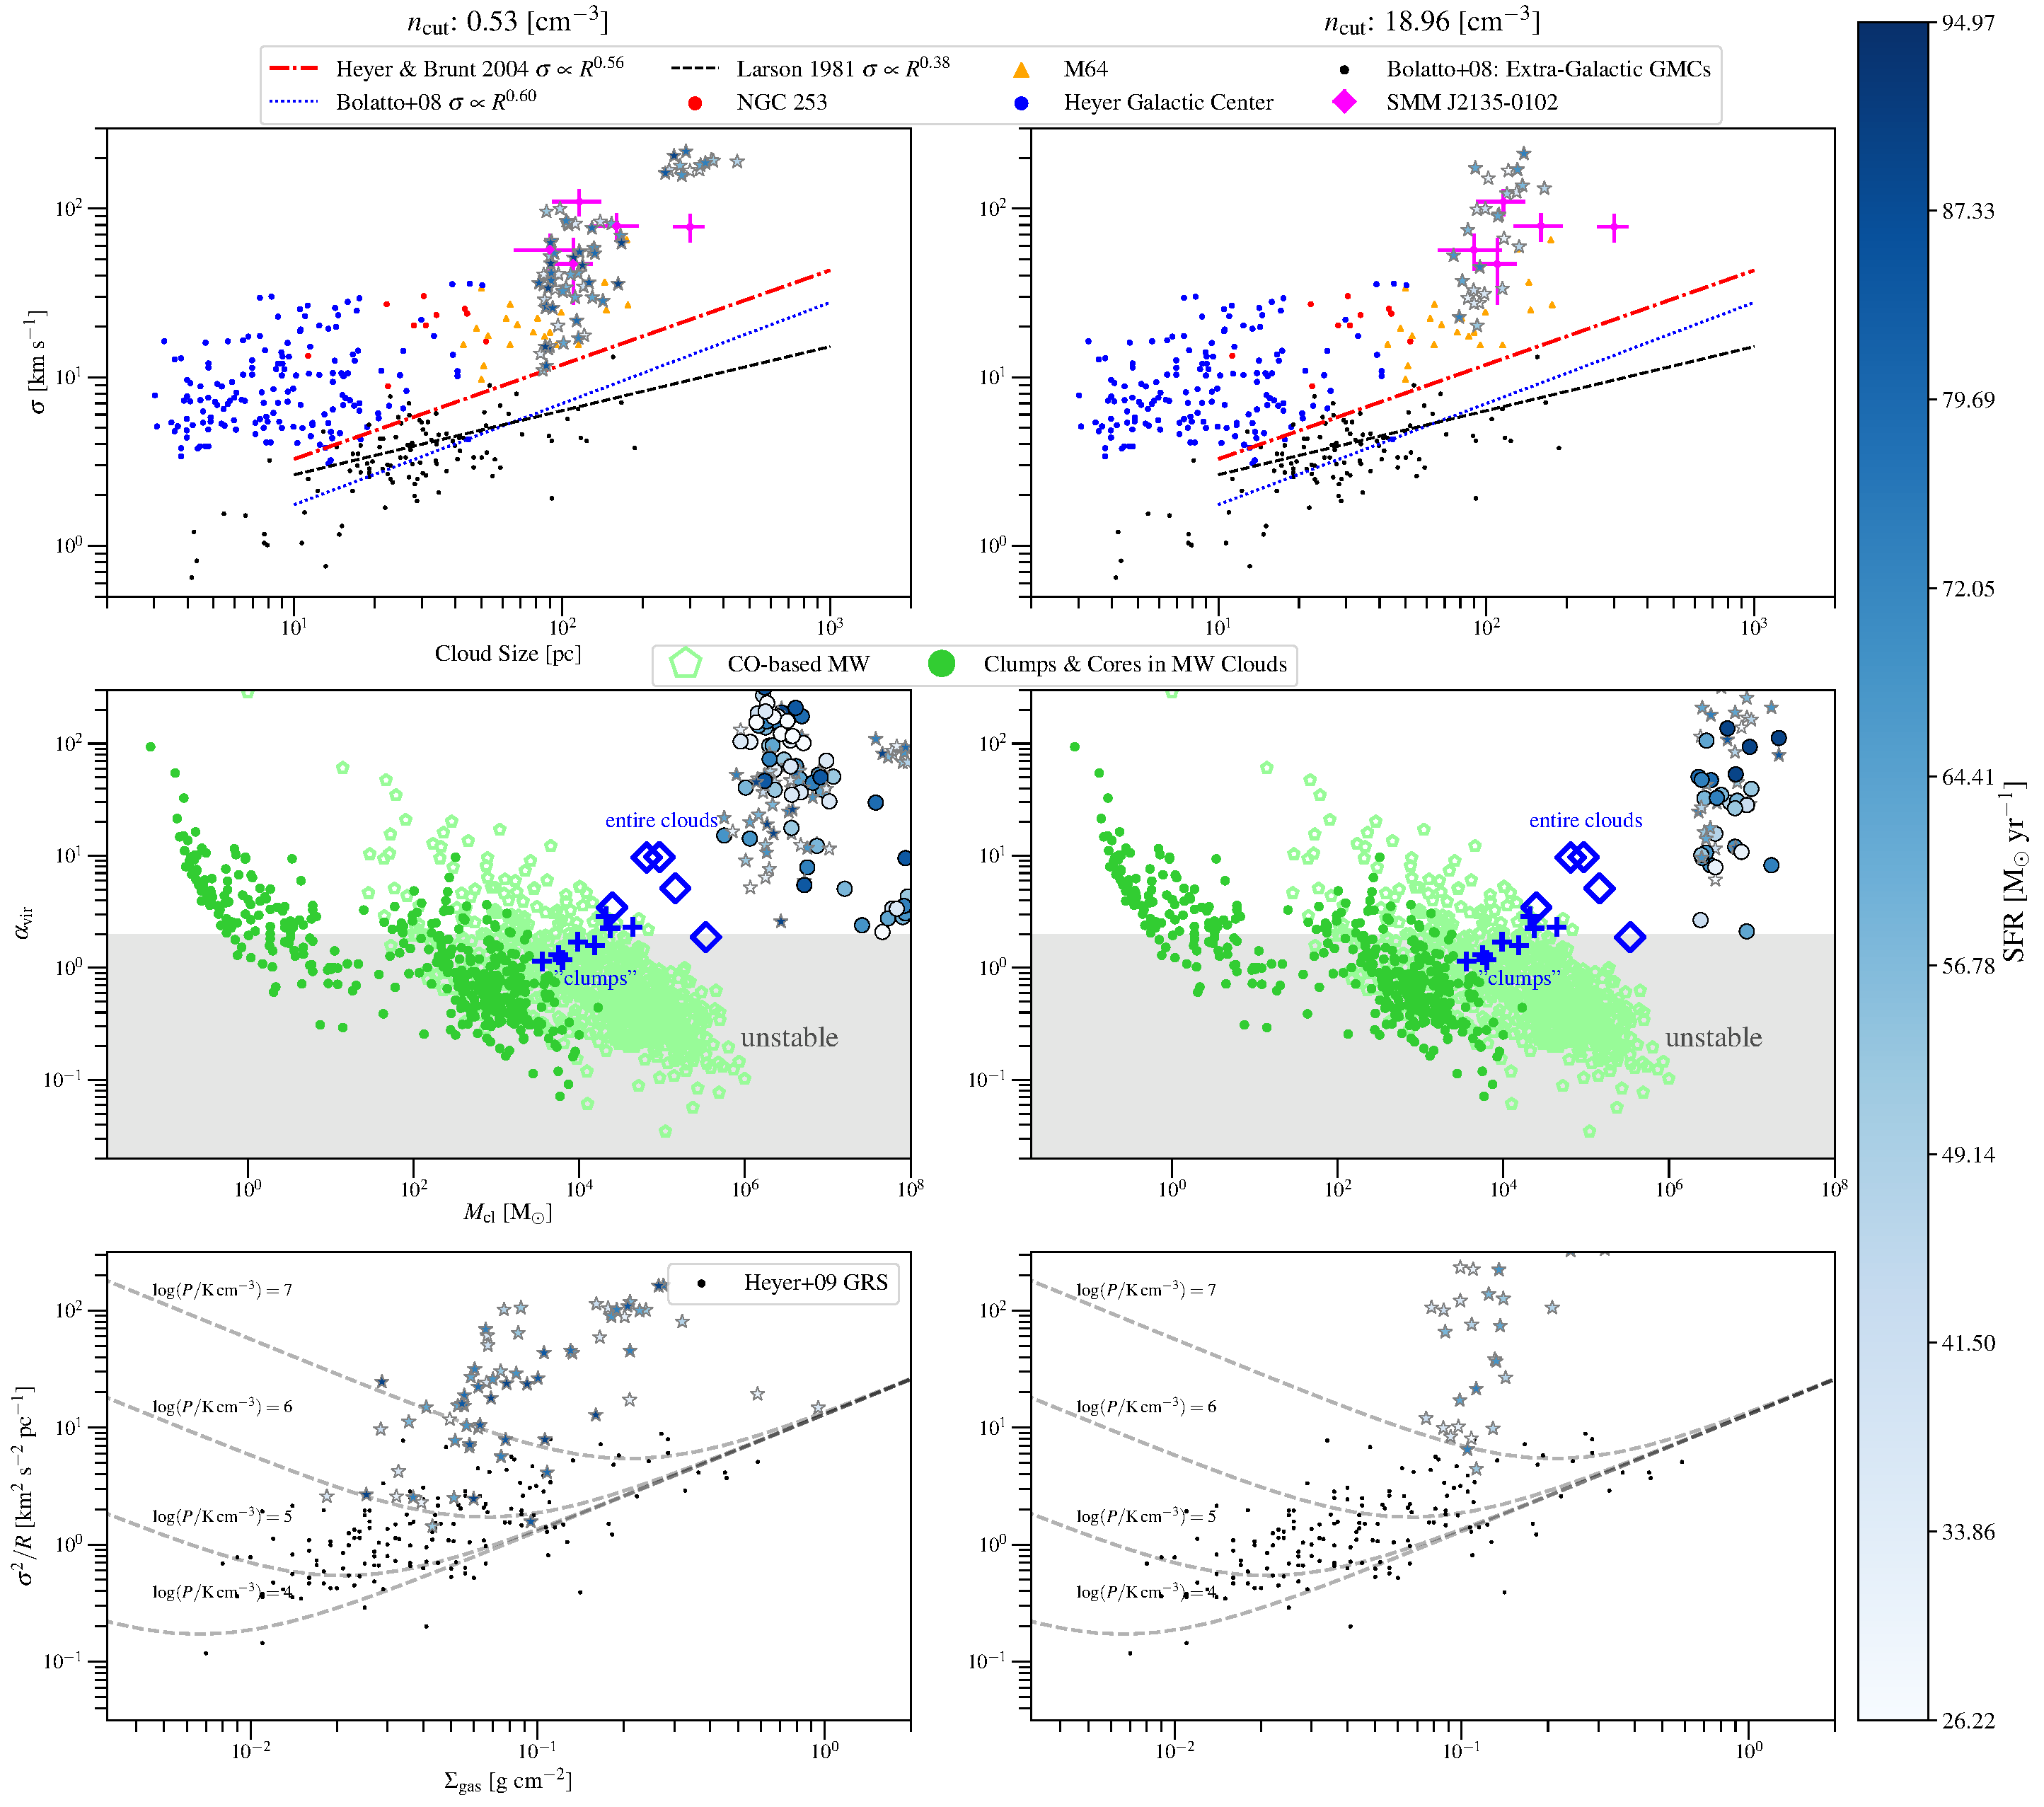
\includegraphics[trim=0 0 0 0, clip, width=1.05\textwidth]{\figpath/3by2_clumpProp_allss}
\caption{Same as \Fig{larsons_single}, except star symbols are showing MCCs identified across all evolutionary stages traced in our simulation, which are color-coded by the SFR of \flower in those stages. Left panels show MCCs identified using a low $n_{\rm cut}$\eq0.53\,\cc and right panels show MCCs identified using a high $n_{\rm cut}$\eq19\,\cc.
\label{fig:alpha16-28}}
\end{figure*}

\subsection{Single Evolutionary Stage}  \label{sec:singless}
\AF{Description of the results is very chaotic. You mix evol. phases, properties, ncut, that is physical and numerical issues. Please reorder and make it more logical.}
We first focus on the two most extreme evolutionary stages of \flower\ --- accretion and starburst phase (see \Sec{sfh}), and identify a set of MCCs in each of them. Scaling relations for the MCCs are shown in \Fig{larsons_single} for the accretion (left panels) and starburst phase (right), respectively. Let us start from analyzing the accretion phase.

MCCs in \flower\ are characterized by large velocity dispersions ($\sigma \approx 100 {\rm km s}^{-1}$) and sizes ($R\approx 100$ pc). These values are consistent with those found in starburst galaxies as SMM J2135-0102, located at $z=...$ \AF{Give refs. here and in caption; in addition it would good to give the properties of this galaxy}.
Sizes are somewhat dependent on the choice of $n_{\rm cut}$. As such density threshold is increased, some of the MCCs within the main disk break into multiple sub-MCCs. In this case, we effectively identify a population of denser molecular structures (see \Fig{MCC}). Instead, we find that $\sigma$ is rather insensitive to the actual value of $n_{\rm cut}$. 

%Now discuss sigma - R relation; poor statistcis. But how many MCCs do we have?


% Starburst 
Some MCCs in the starburst phase have lower velocity dispersion, $\alpha_{\rm vir}$, and $\sigma^2/R$ (closer to loci with lower external pressure) compared to the accretion phase. \DL{Is this significant enough to say something physical? If so, not immediately clear to me what cause the differences.}
% PVE
We also compare the MCCs identified in our simulations to those observed in the Milky Way in the context of the $\sigma^2/R - \Sigma$ relation (see bottom panels of \Fig{larsons_single}). Dashed lines in the figure show the loci along which the given external pressures are needed for MCCs to have certain linewidths for a given set of surface densities (see \Sec{PVE}).
% (Rice+16) find variation in $V_0^2$, where they find larger linewidths for GMCCs in inner galactic disk, but they find that the clouds in the Galactic disk are still consistent with SVE (see also Solomon87a ; cf. Heyer+09).
The MCCs in the satellite galaxies are found to follow the locus of $\log{(P/\textrm{K cm}^{-3})}$\eq6, which
is consistent with that found for the bulk of dense gas in the simulation in the phase-space analysis presented in \citet{Pallottini17a}.

% cloud structures at large and small scale
% Larson's: m = 460 M_sun (r_pc)^1.9 for structure w/in molecular clouds. --> $m \propto r^2$ \citep{McKee07a} (law of constant
% column density) as fundamental properties of molecular cloud structure.
Larson's third relation relates MCCs structures on small and large scales via two physical properties: mass and size \citep{Larson81a, McKee07a}. This is also known as the constant column density relation, since cloud mass in \obs is sometimes derived by integrating over the mass surface density, which is related to the column density ($N_H$) obtainable from extinction maps ($A_V$). By assuming dust properties from \citet[][]{weingartner:2001}, extinction for a cloud with Milky Way-like dust can be written as 
\begin{equation}
A_v = \frac{N_H}{1.8 \times 10^{21} {\rm cm}^{-2}}\,,
\end{equation}
then, assuming spherical symmetry, the mass of an MCC can be expressed as a function of $A_v$ and its size $R$
\begin{equation}\label{eqn:constantcolumndensity}
M_{\rm cl} = \frac{4\pi}{3} \mu m_p n R^3 = 154~A_v \left(\frac{R}{\rm pc}\right)^2 \Msun \,,
\end{equation}
where we have taken $\mu = 2.5$ as the mean molecular weight.

We show in \Fig{MR} the size-mass relation of the MCCs of \flower compared to observational data of molecular clouds in the Milky Way that are found to be associated with massive \SF \citep{Beuther02a, Mueller02a, Hill05a, Motte07a} and an empirical relation obtained for massive \SF based on Milky Way clouds ($<$10\,\Msun; \citealt{Kauffmann10b, Kauffmann10c} and references therein): $M \gtrsim 870(R/{\rm pc})^{4/3} M_\odot$.
%
In the same plot, we also show loci of constant surface densities, which are parameterized through the visual extinction $A_V$. As shown in \Fig{MR}, the MCCs identified in \flower lie above this relation, along the locus of $A_v \simeq 8.9$ clouds observed by \citet{Lombardi10a} in the MW.
%
%The values of $A_V$ inferred from http://adsabs.harvard.edu/abs/2017MNRAS.471.5018Fthe $M_{\rm cl}$-size relation is consistent with the extinction inferred from gas clumps analysing the UV and IR emission of \flower~by calculating the effect of radiative transfer through dust \citep[][in particular see Fig. 5 therein]{Behrens18a}

\begin{figure*}[htbp]
\centering
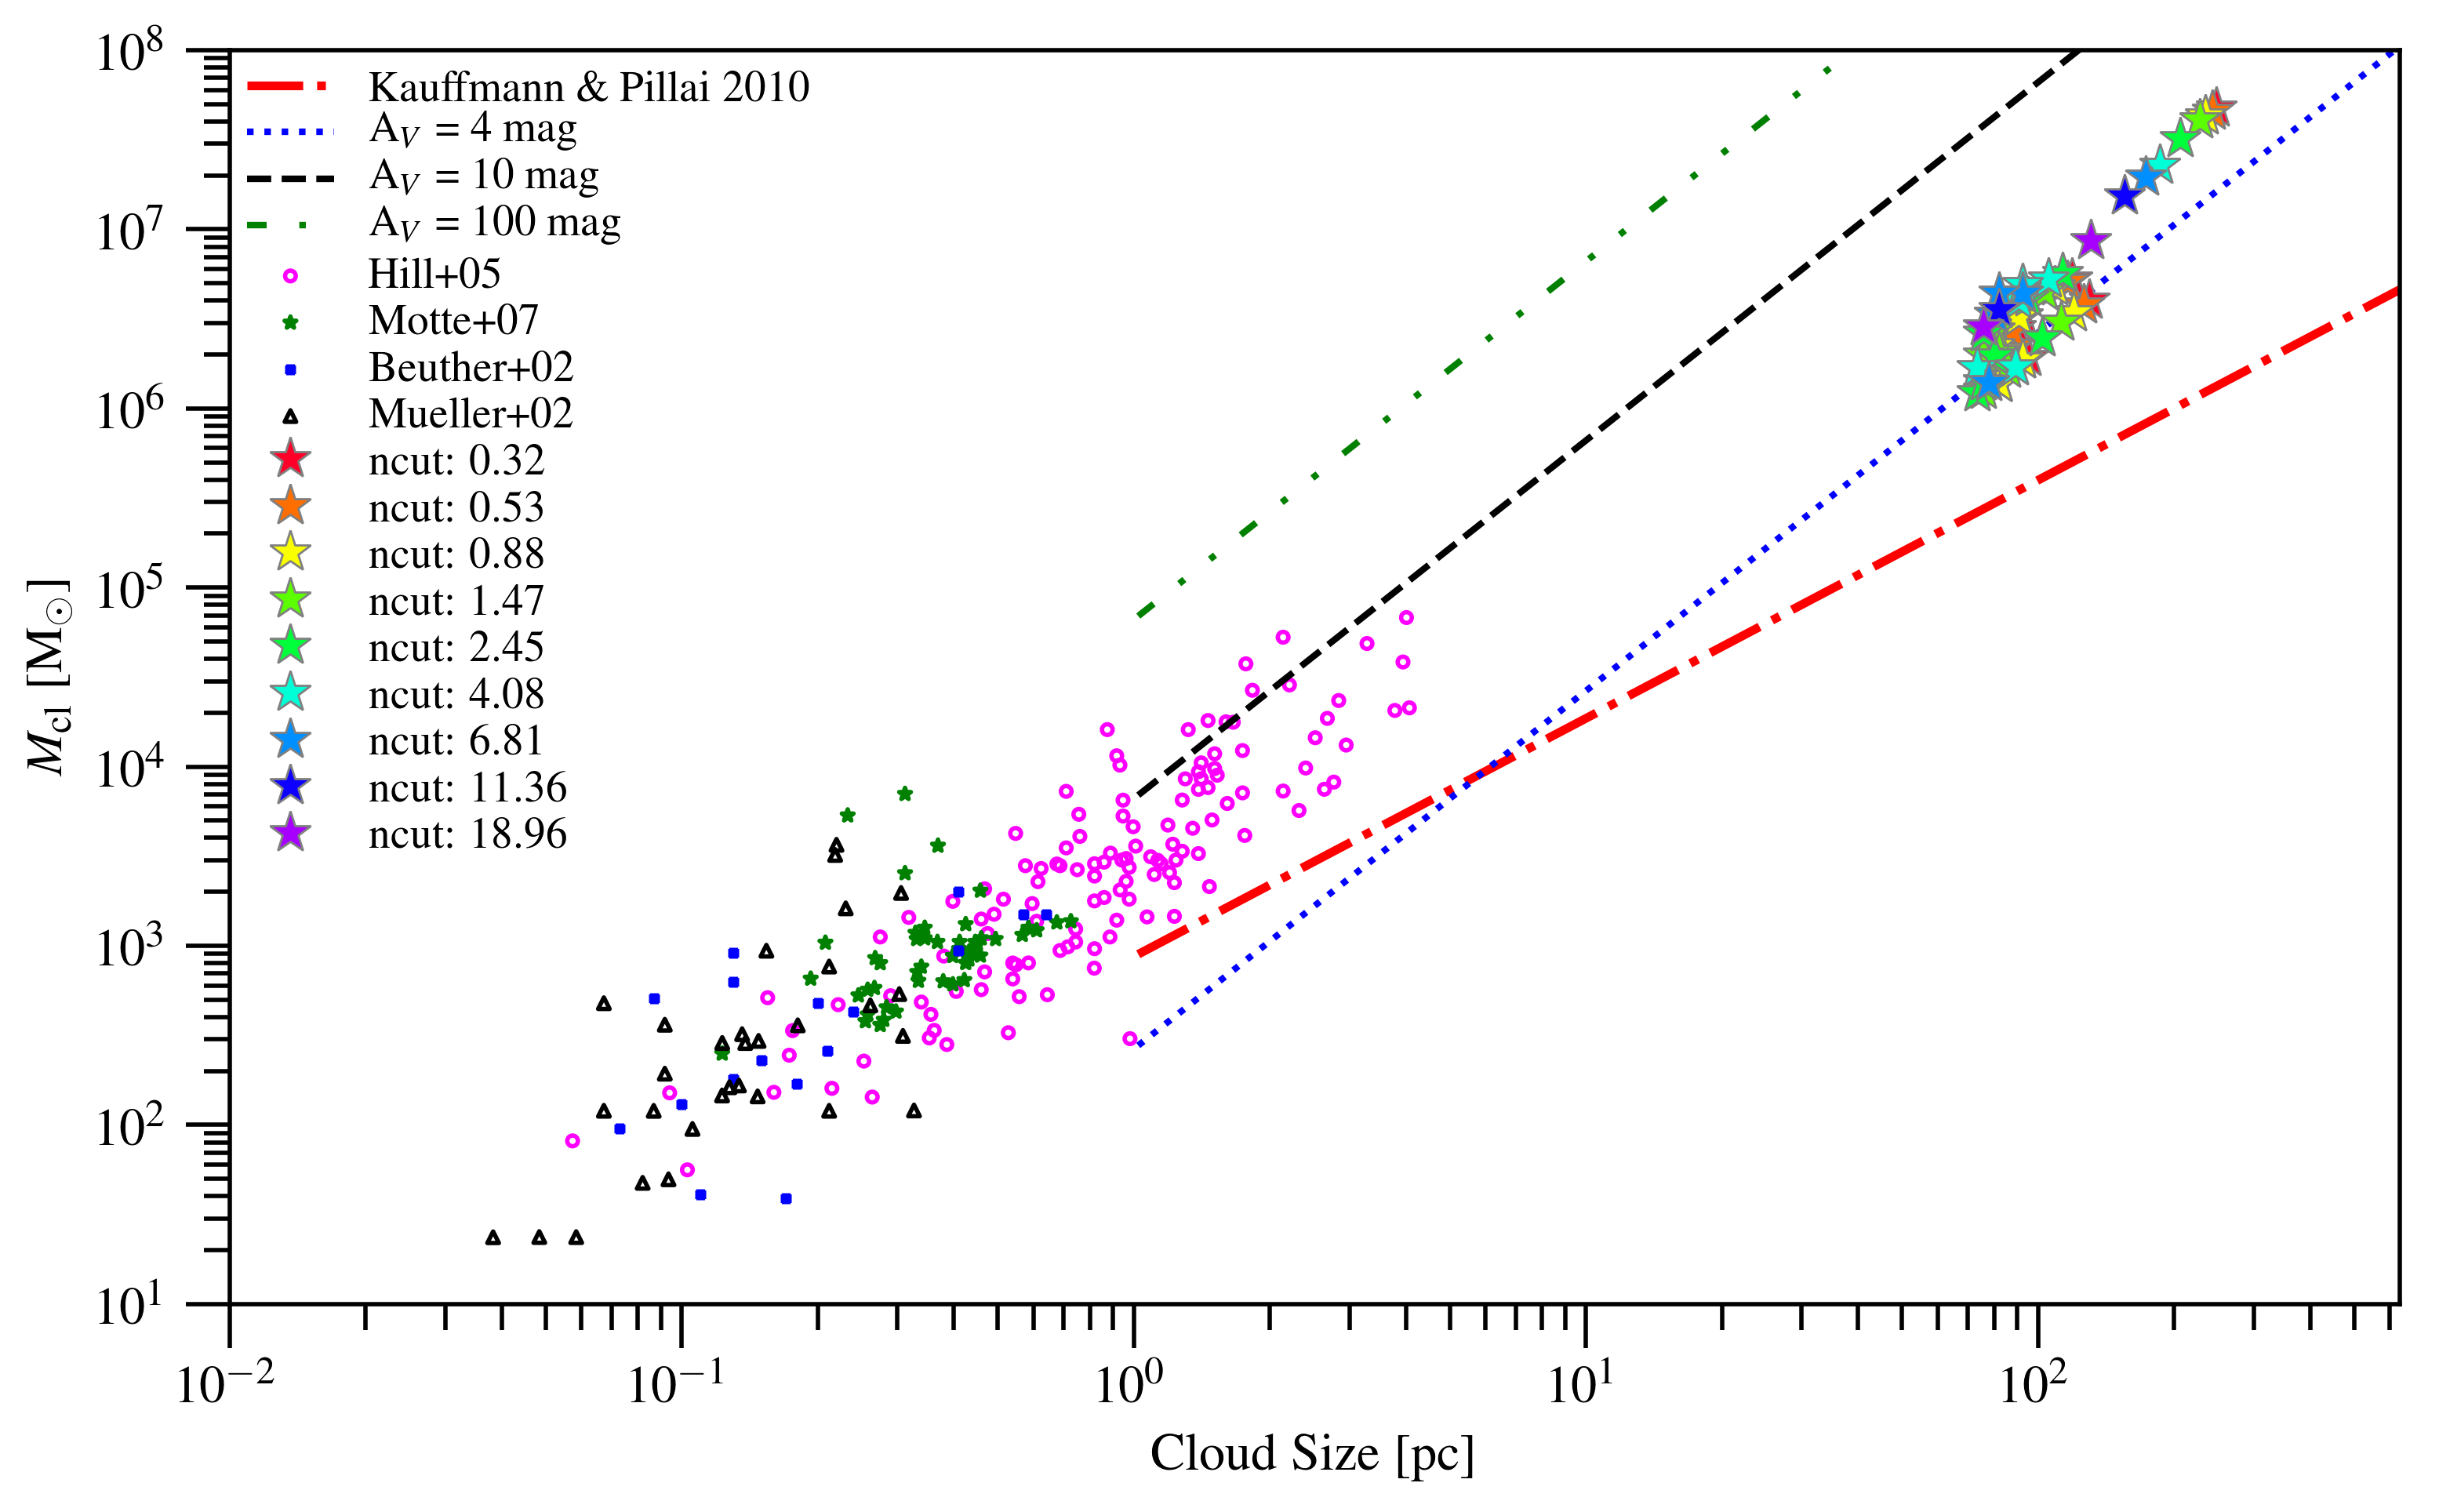
\includegraphics[trim=0 0 0 0, clip, width=0.8\textwidth]{\figpath/lf16_cloud-mass_size-pc.png}
\caption{
Size-mass relation of MCCs identified in the accretion phase of \flower in our simulation (star symbols) compared to observational data of molecular clouds in the Milky Way associated with massive \SF (magenta circles, green stars, blue dots, and black triangles) and empirical relations established based on \obs of the Milky Way. Red line shows the 
mass-size relation found for regions in the Milky Way with massive \SF reported by \citet{Kauffmann10b}. Star symbols are color-coded by increasing $n_{\rm cut}$. Literature data are compiled from \citet{Beuther02a, Mueller02a, Hill05a, Motte07a}. 
Colored lines show the loci expected for different visual extinctions ($A_V$, see \Eq{constantcolumndensity}), which correspond to lines of
constant surface density (i.e., Larson's third relation). This representation is motivated by observational studies (see text and e.g., \citealt{Lombardi10a}).
The star symbols are color-coded by $n_{\rm cut}$, same as \Fig{larsons_single}. 
Extrapolating the masses and sizes of MCCs of \flower along the \citet{Kauffmann10b} 
relation down to 1\,pc are comparable  to those  of  the  cores  found  in regions  of high-mass star formation, suggesting that the identified MCCs are capable of high-mass \SF.
\label{fig:MR}}
\end{figure*}

\subsection{Temporal Evolution and Adopted Density Threshold Dependence}\label{sec:ncut}
% single Snapshot
We investigate possible variations in the dynamics of the molecular structures of \flower and its satellites to test the robustness of our results against the choice of density threshold by adopting different sets of $n_{\rm cut}$ in identifying the MCCs. That is, how sensitive are the structure properties, and thus, the results presented in \Sec{singless} dependent on the choice of density thresholds.
%
We vary the choice of H$_2$ density for each of the evolutionary stages and find no obvious differences in our results, i.e., inferences on the dynamics of \z$\sim$\,6 MCCs in relation to those observed in nearby and \z$\sim$2 galaxies in the context of cloud scaling relations.
%
In addition, for the densest MCC in the main disk of \flower, we find that while its size decreases as we increase $n_{\rm cut}$ --- as one would intuitively expect, the velocity dispersion remain approximately $\sigma\simeq$\,200\,\kms (see also \Fig{larsons_single}).
%
This lack of variation is reassuring, i.e. the dynamics of the MCCs are not artifacts or biased by our choice of $n_{\rm cut}$ on the scales studied in the present work. Our results are therefore robust to the various density cuts of choice.

% temporal evolution in Cloud Dynamics
We show the properties of all MCCs identified across all evolutionary stages in \Fig{alpha16-28}. We find no quantitative differences in the cloud properties over the 700\,Myr traced in our simulation.

%
%\begin{comment}
%\begin{figure*}[htbp]
%\centering
%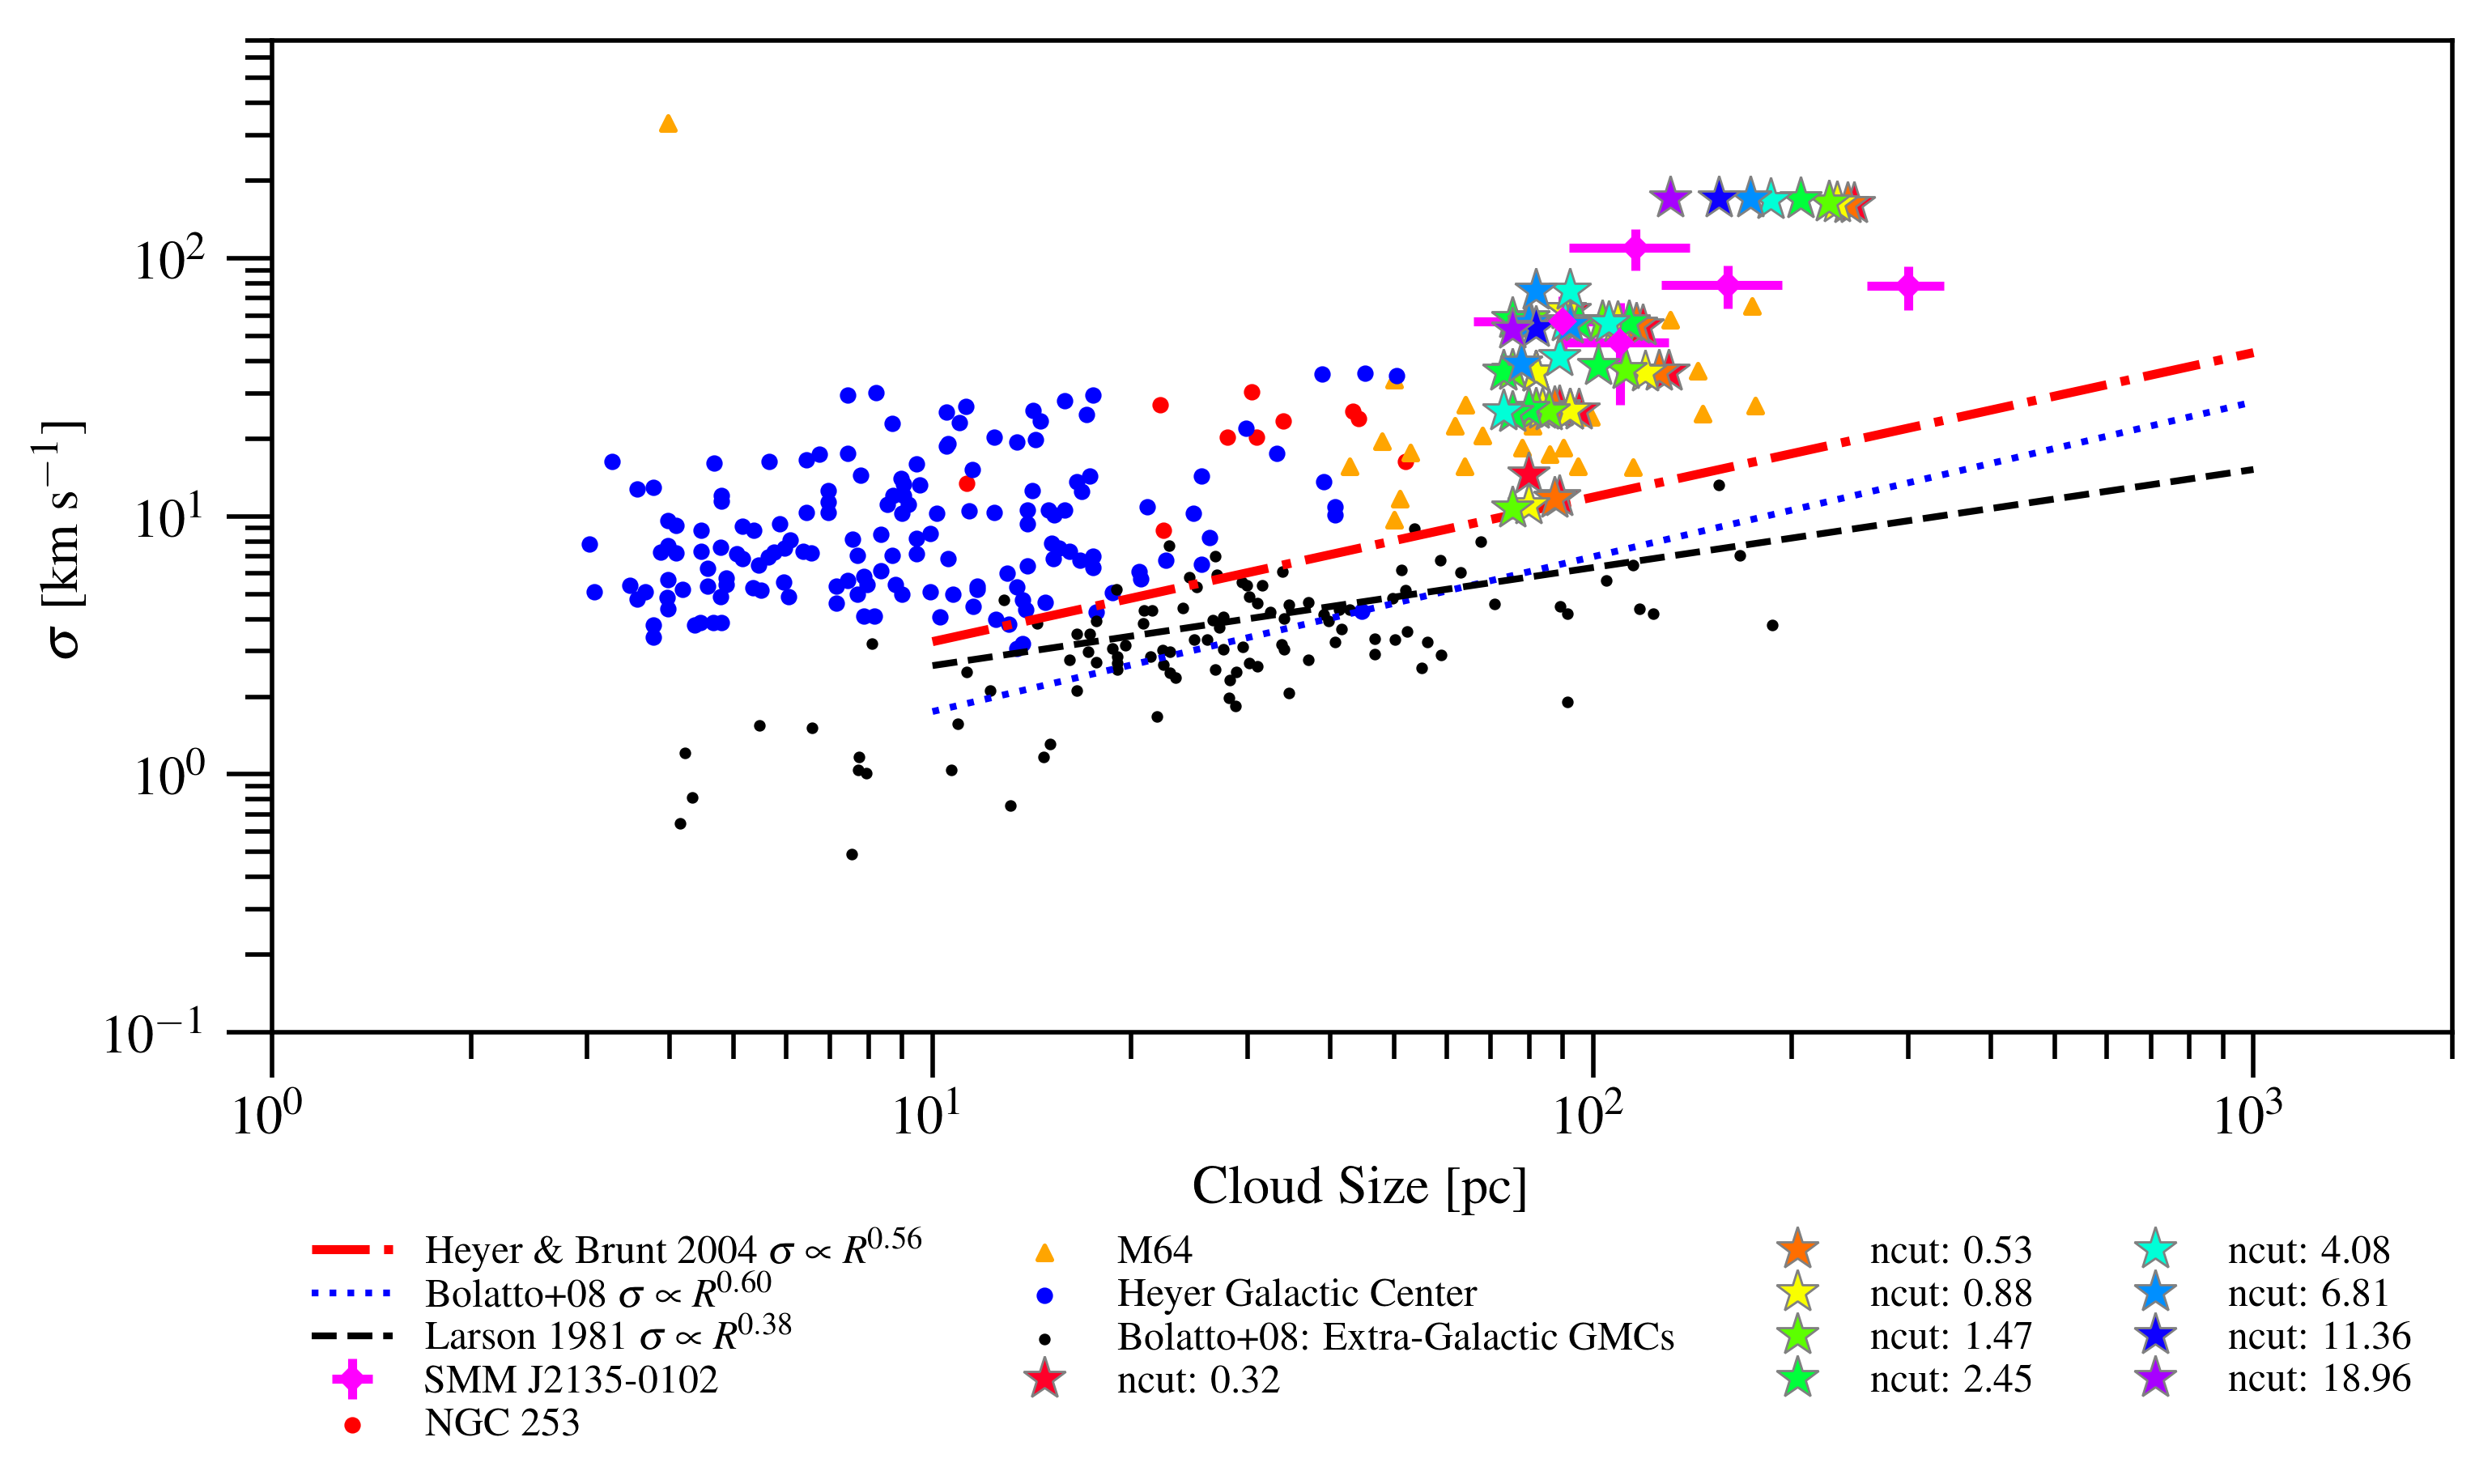
\includegraphics[trim=0 0 0 0, clip, width=0.85\textwidth]{\figpath/ss16_larsons.png}
%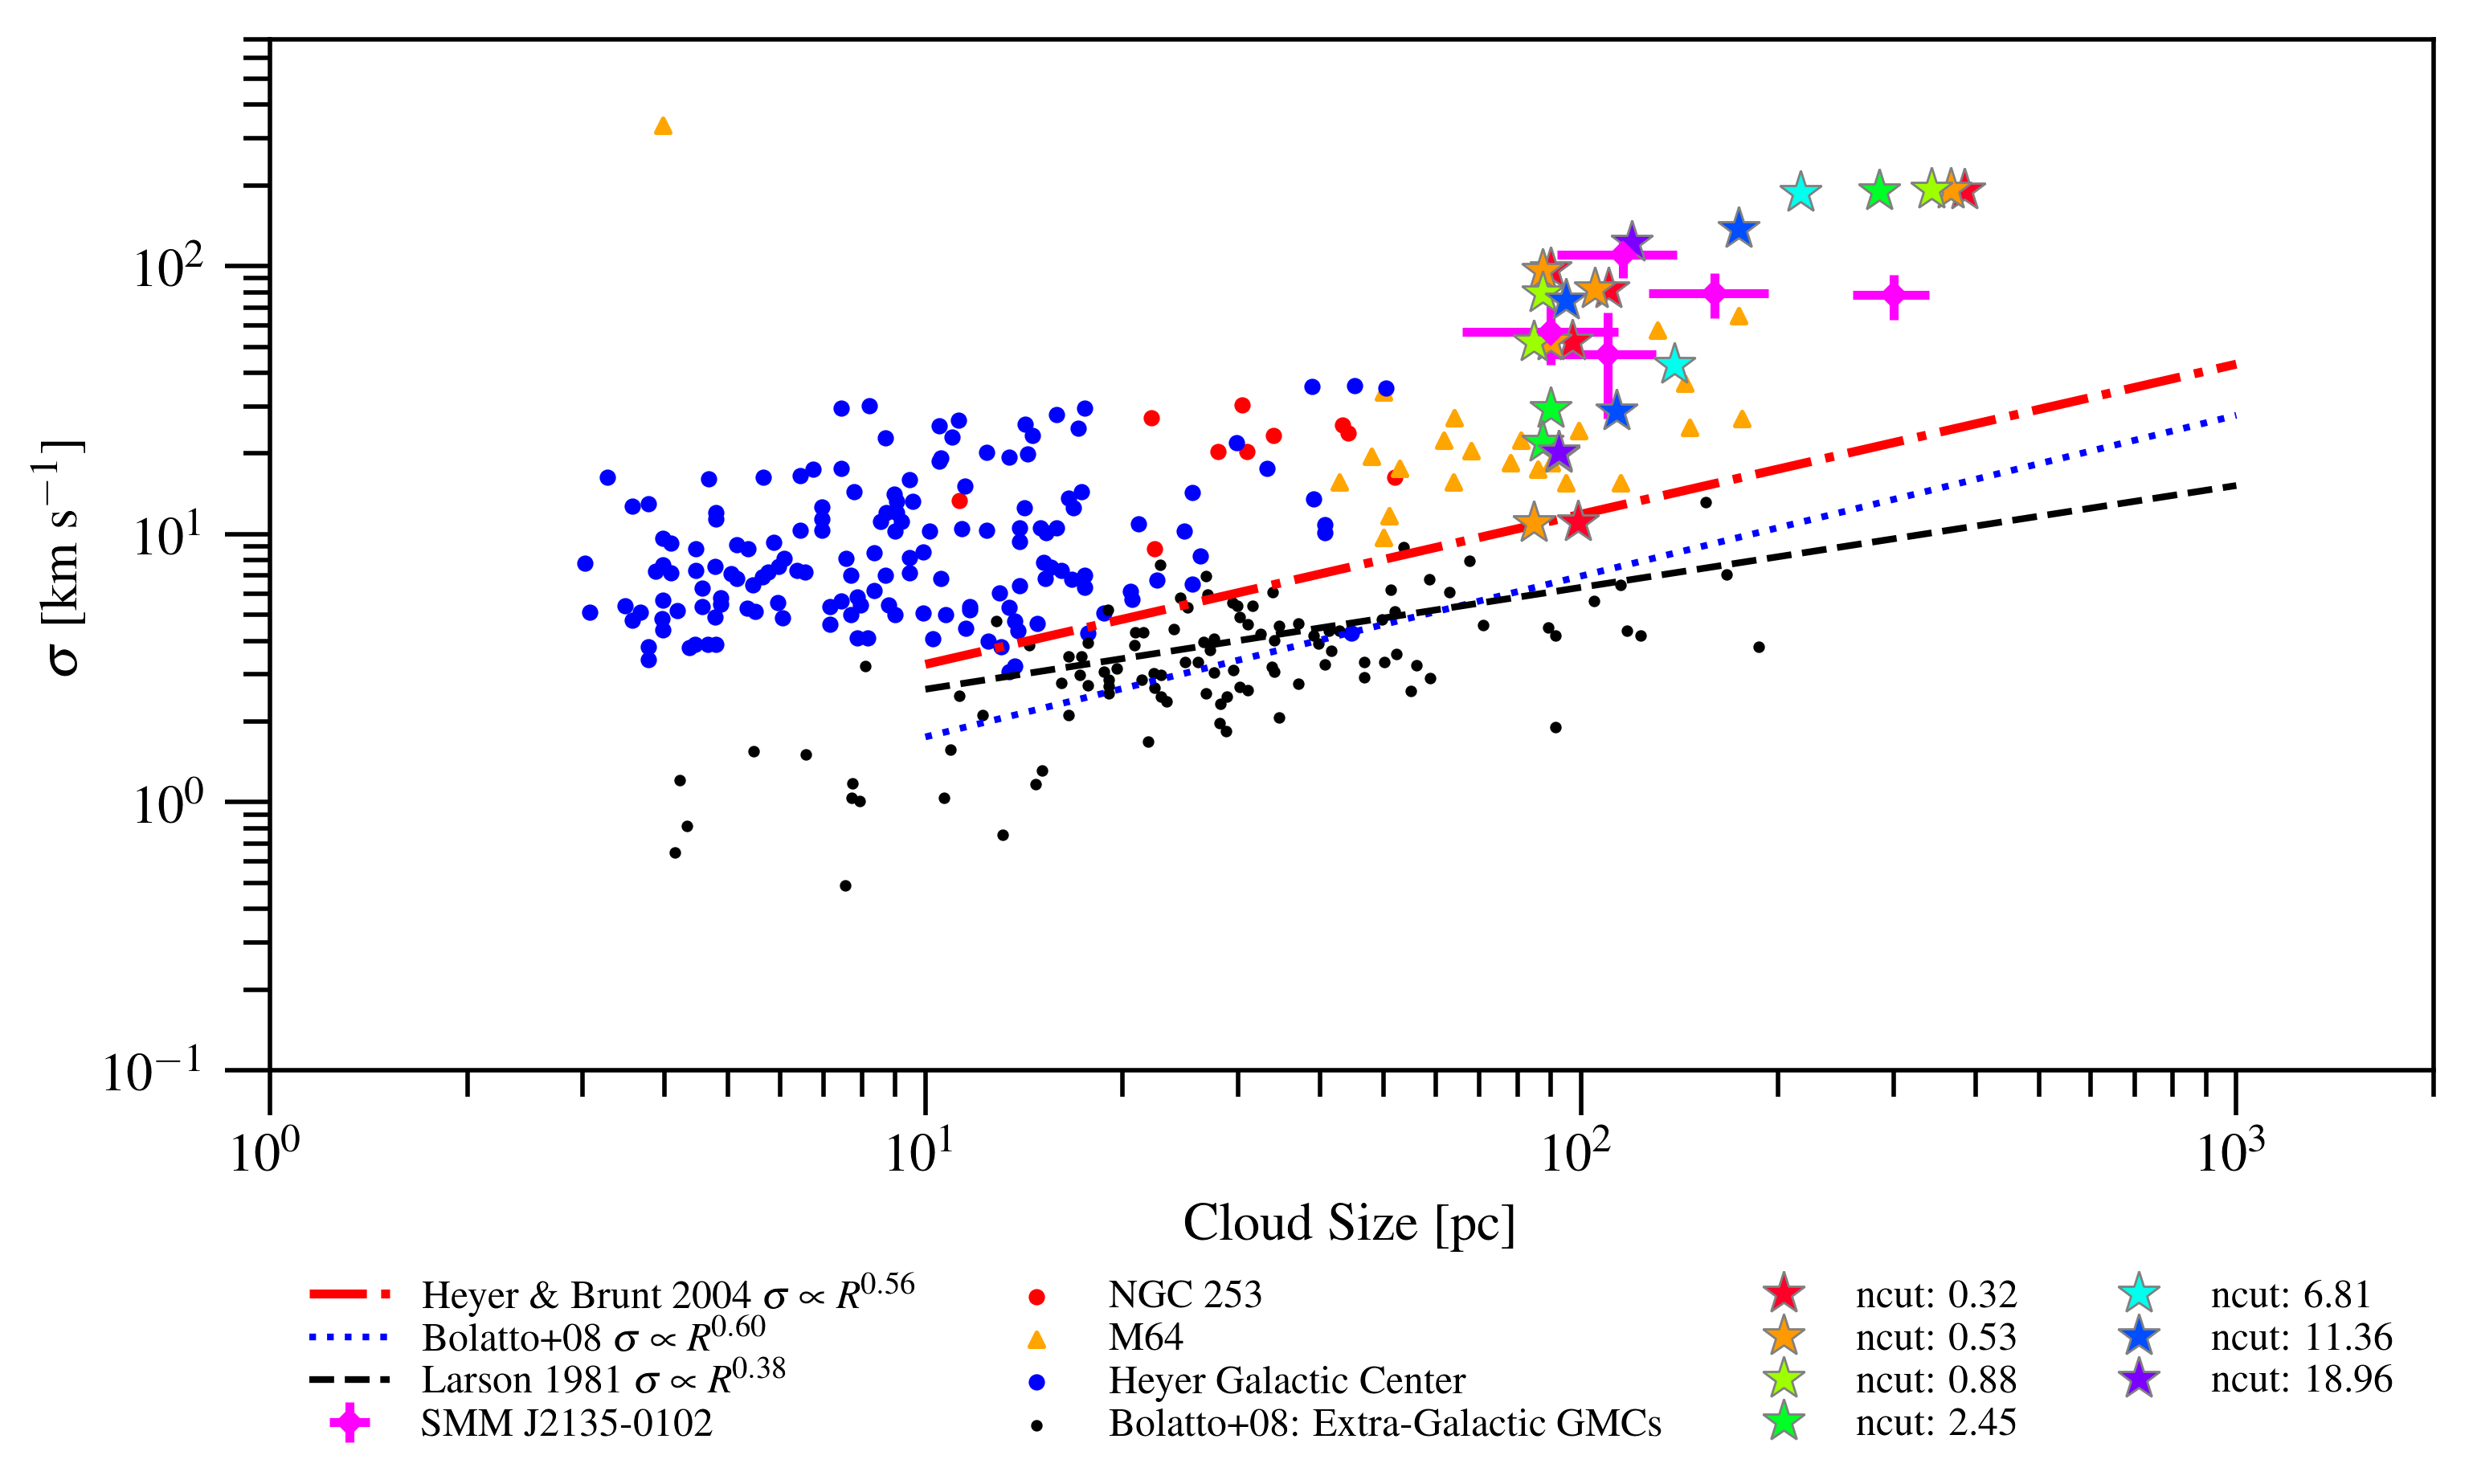
\includegraphics[trim=0 0 0 0, clip, width=0.85\textwidth]{\figpath/ss27_larsons.png}
%\caption{
%Larson's (linewidth-size) relation of \flower in
%accretion phase (top) and
%starburst phase (bottom) compared to
%those observed in nearby and the \z$\sim$2 star-forming galaxy.
%% Red lines show the relation obtained from \citet{}.
%Observed data and empirical relations are compiled from \citet{Larson81a, Heyer04a, Rosolowsky05a, Bolatto08a, Swinbank11a, Leroy15a}.
%\label{fig:larsons_single}}
%\end{figure*}
%
%\begin{figure*}[htbp]
%\centering
%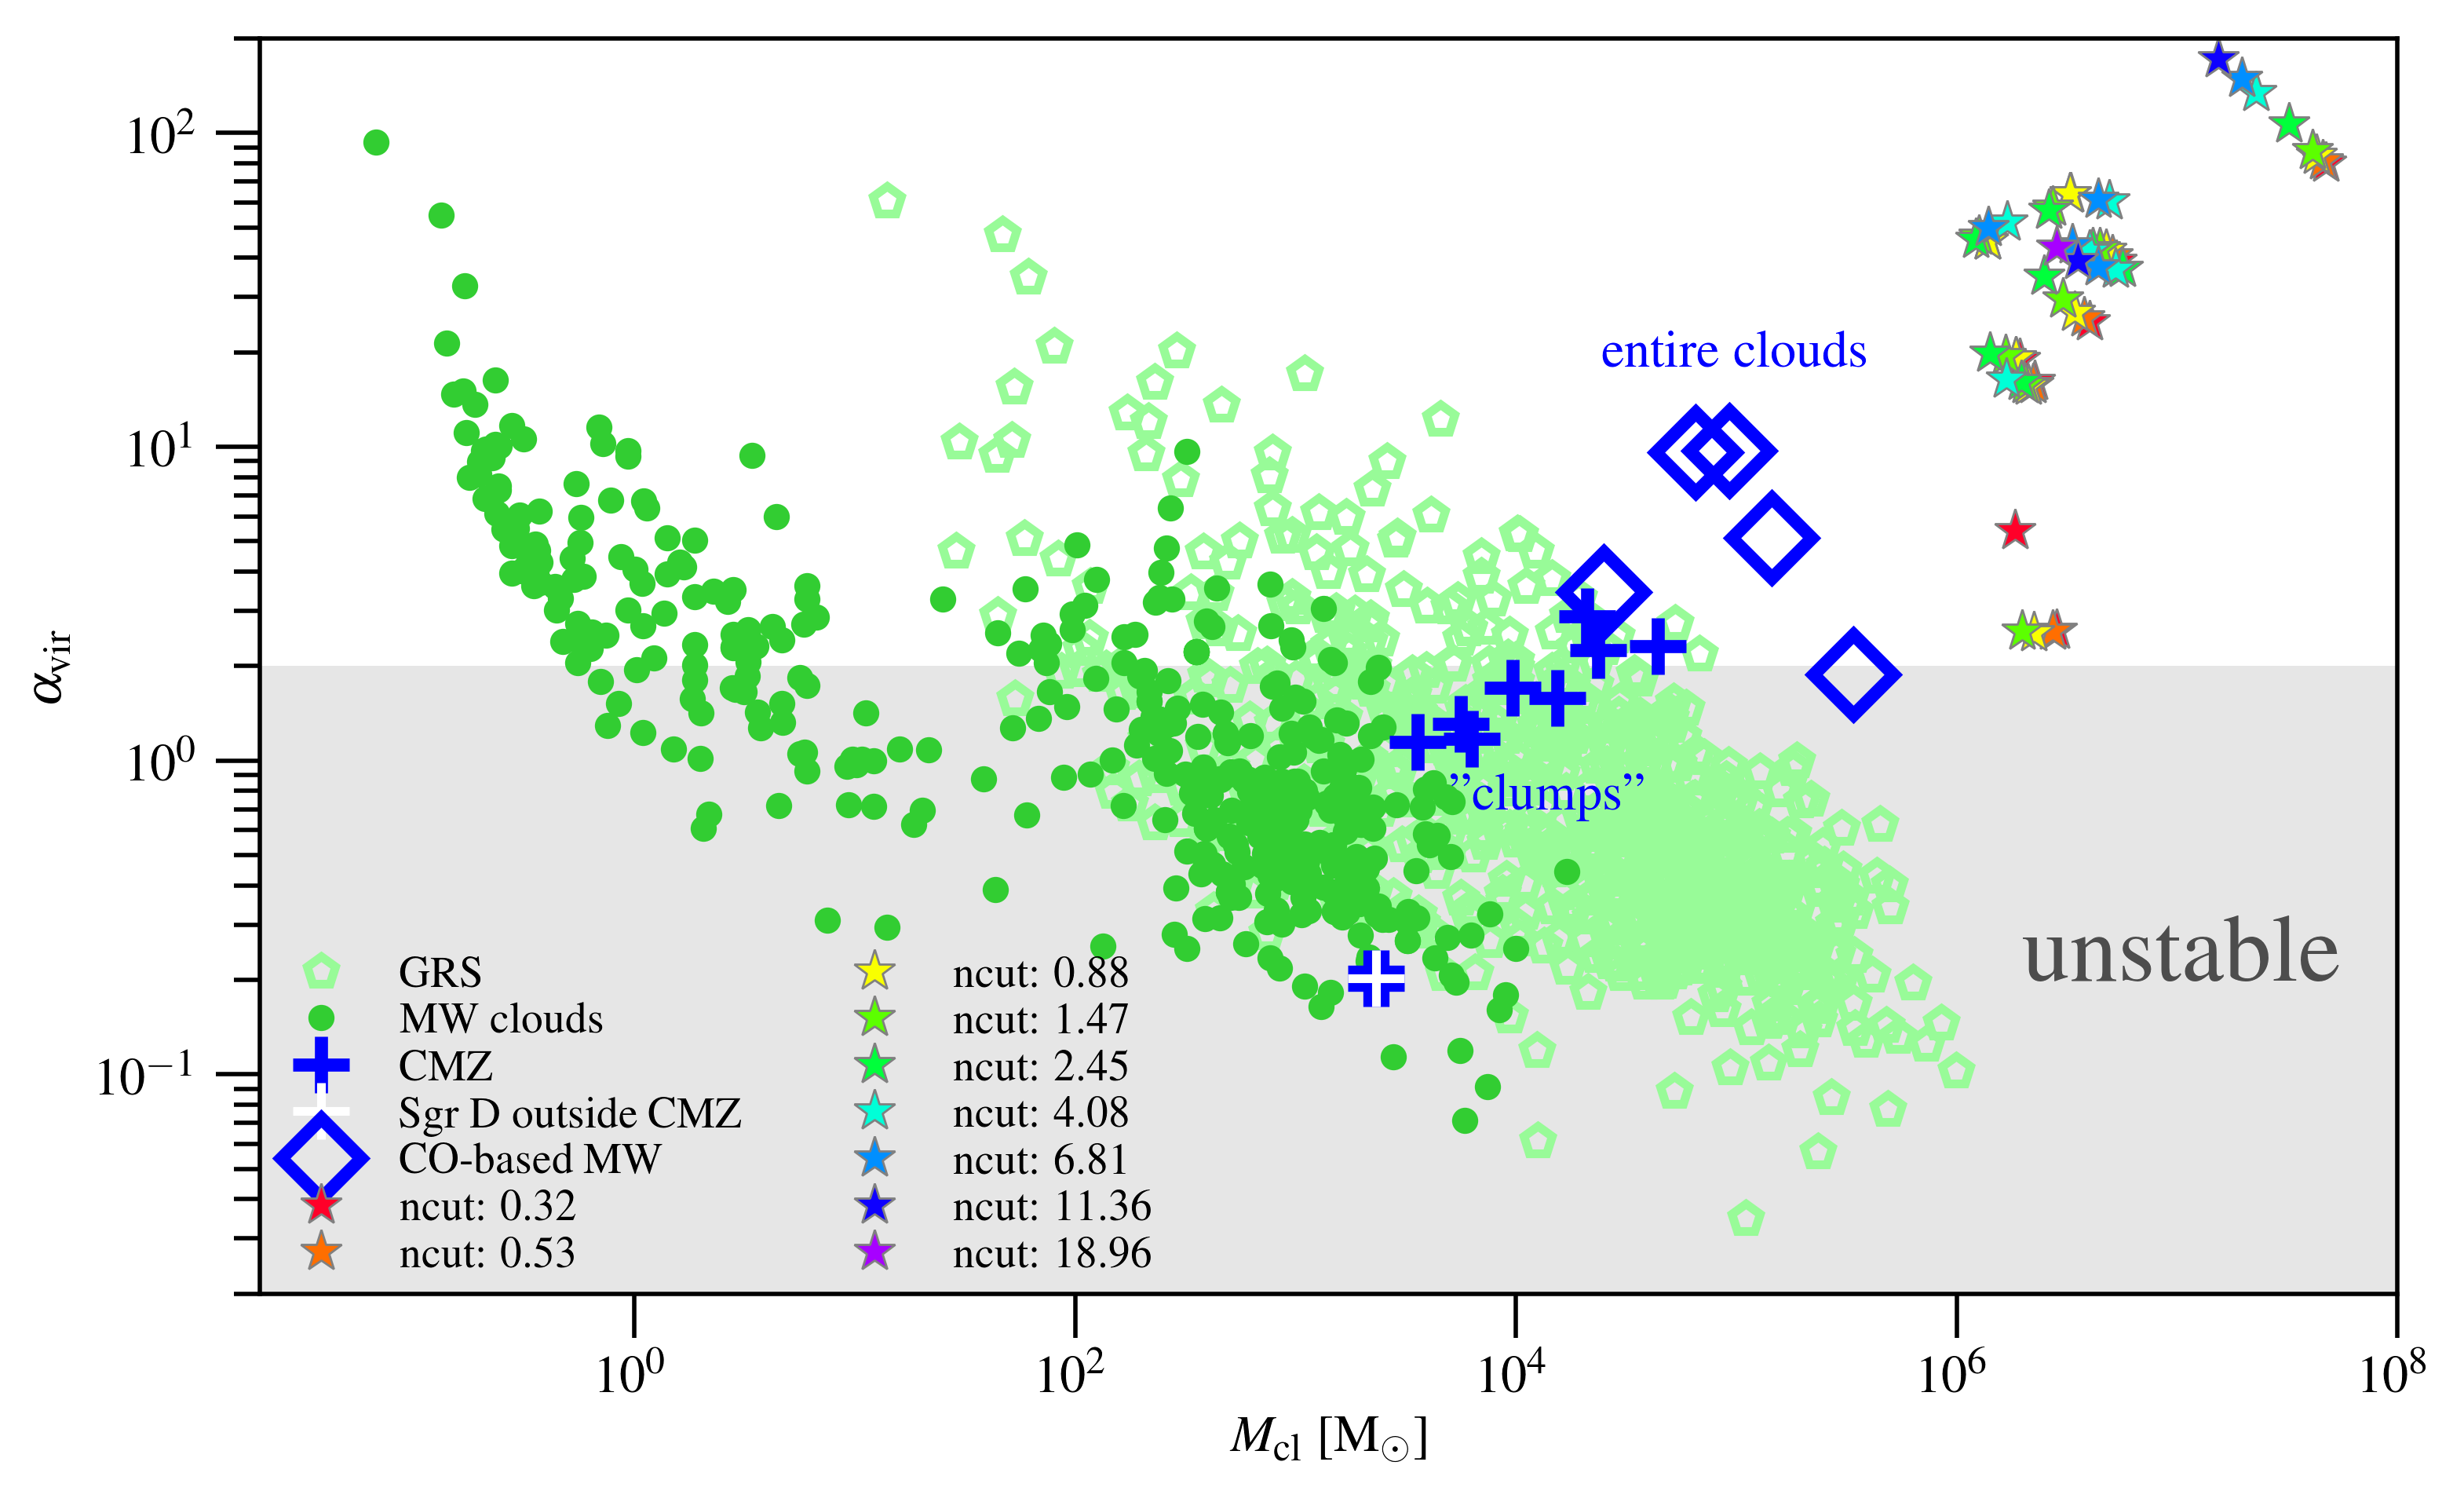
\includegraphics[trim=0 0 0 0, clip, width=0.65\textwidth]{\figpath/ss16_alphavir.png}
%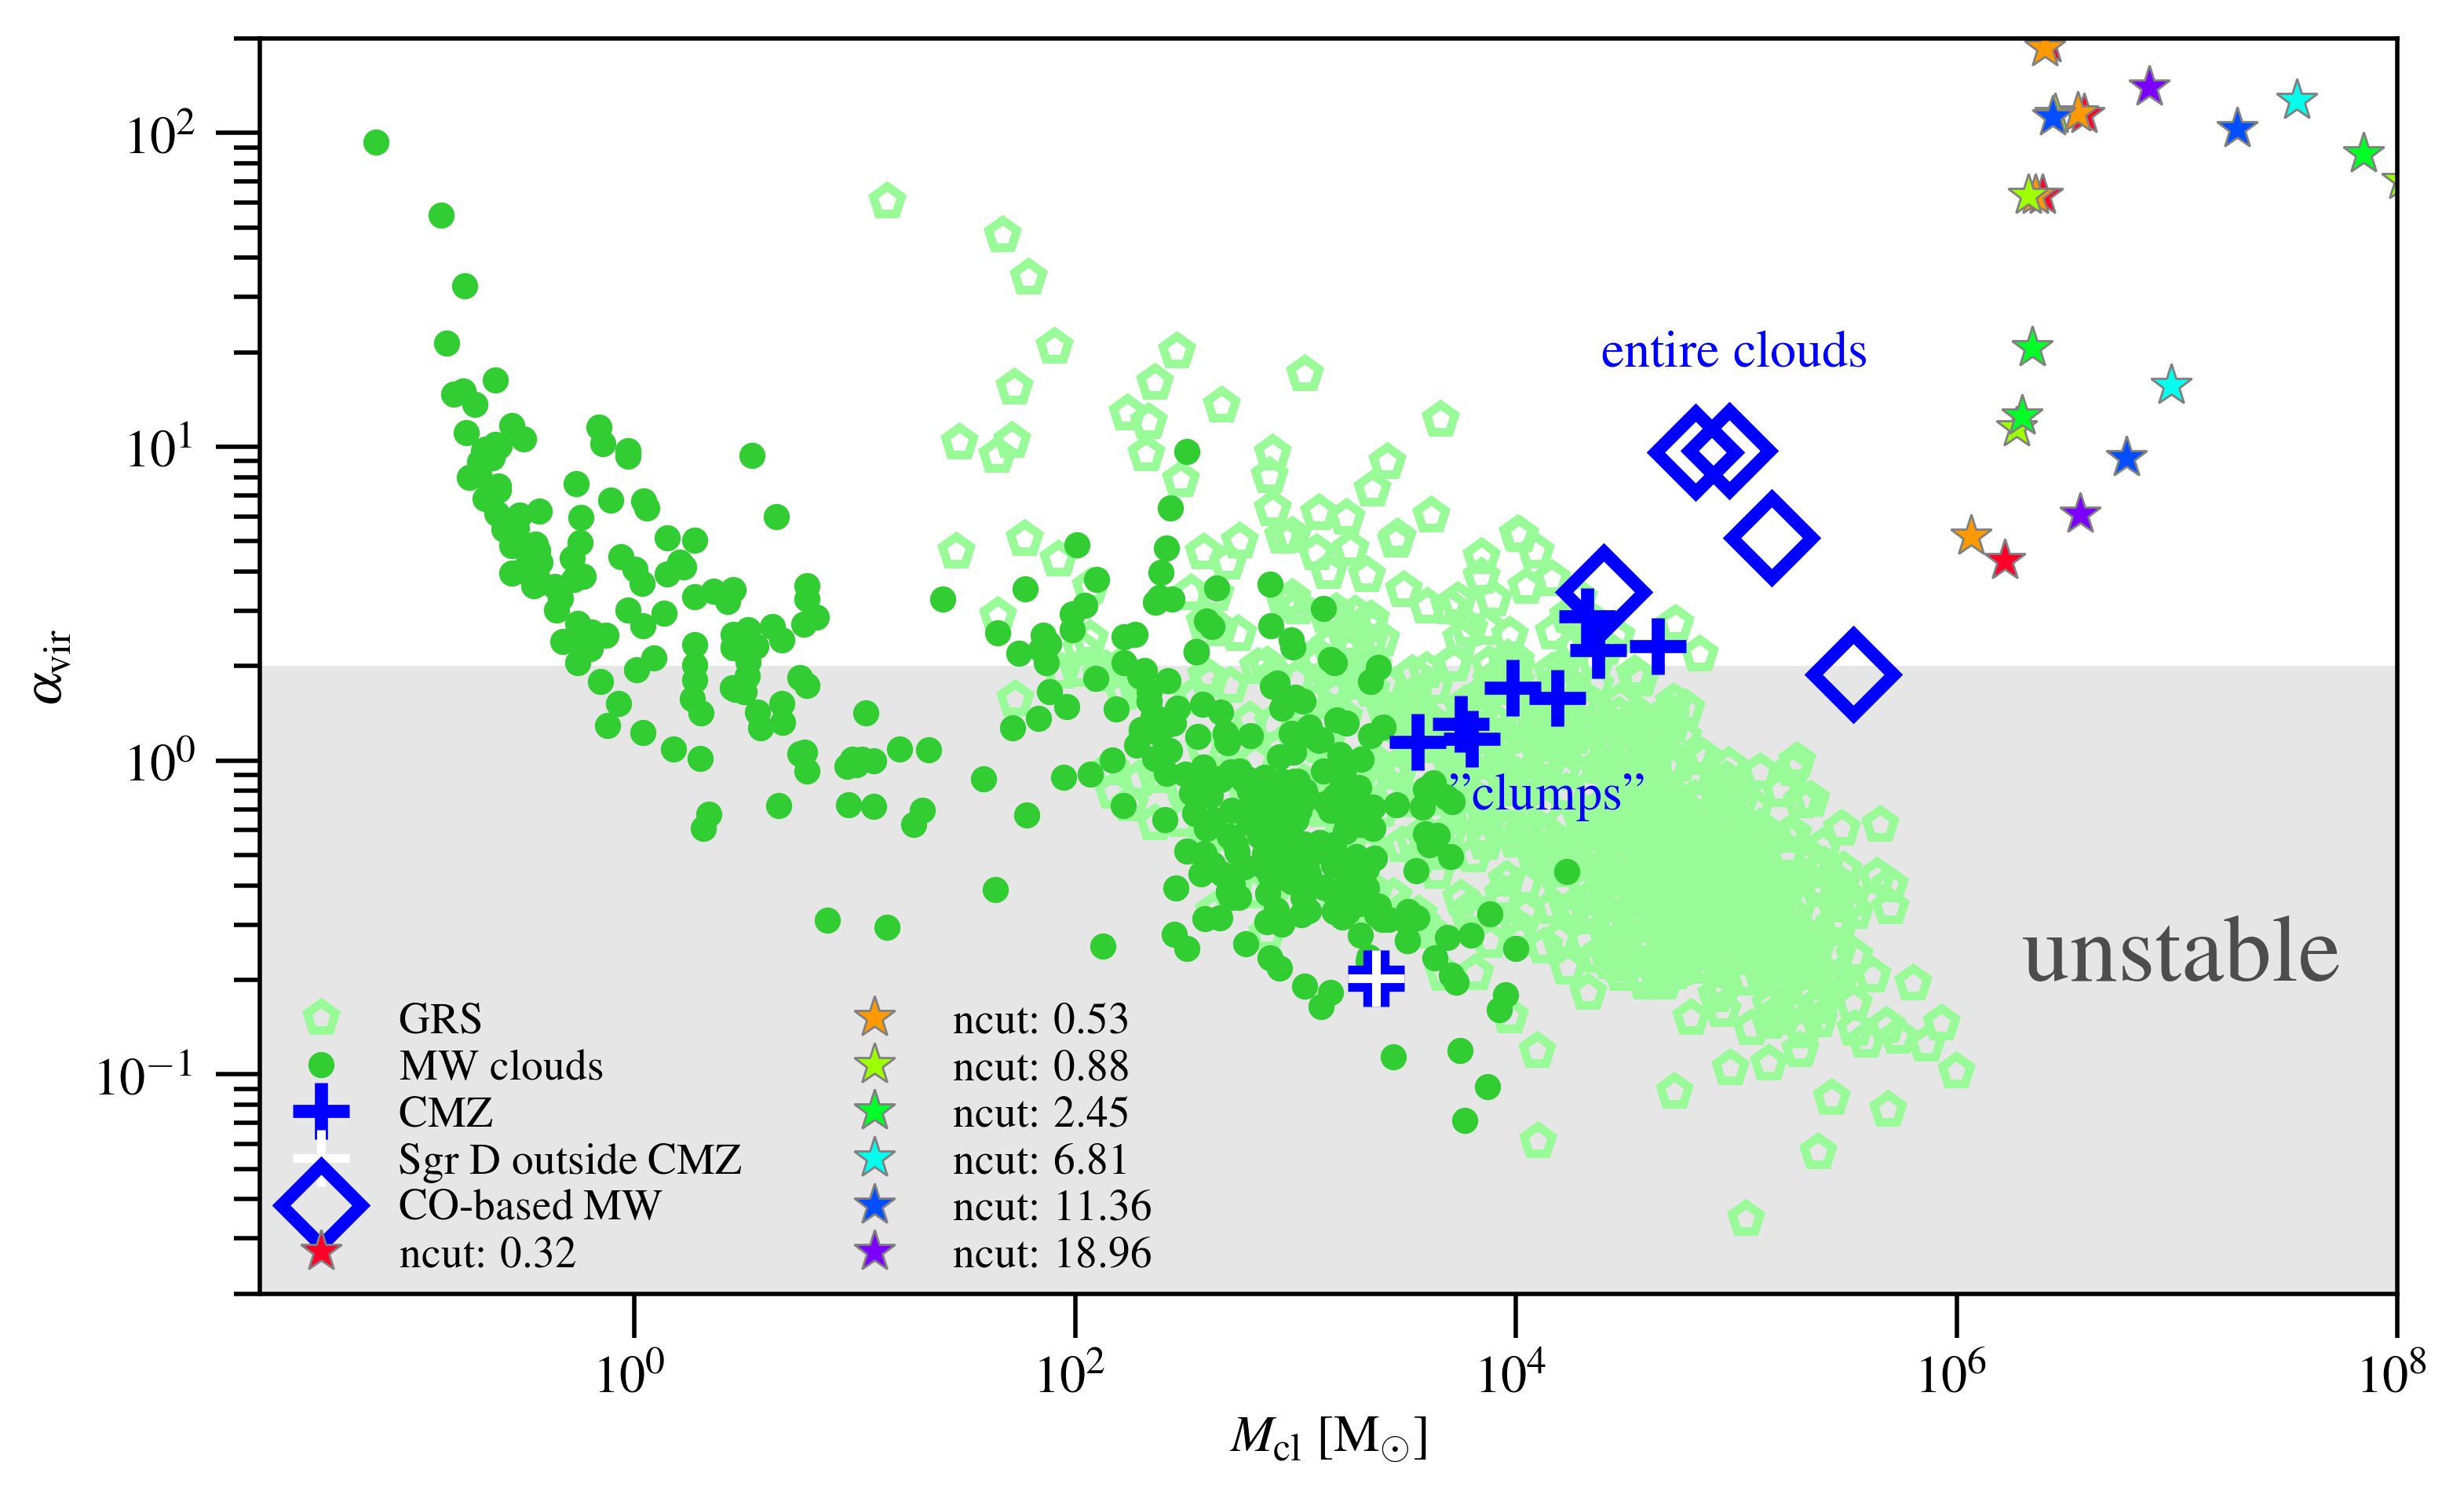
\includegraphics[trim=0 0 0 0, clip, width=0.65\textwidth]{\figpath/ss27_alphavir.png}
%\caption{
%Virial parameter and cloud mass of \flower (star symbols) in the accretion phase (top panel)
%and the starburst phase (bottom panel) compared to the
%Milky Way (other symbols).
%Literature data are compiled from \citealt{Kauffmann17b} and references therein.
%Star symbols are color-coded by $n_{\rm cut}$.
%Star symbols lying close to $\alpha_{\rm vir}\approx2$ correspond to MCCs in the satellite galaxies.
%\label{fig:alpha16}}
%\end{figure*}
%
%\begin{figure*}[htbp]
%\centering
%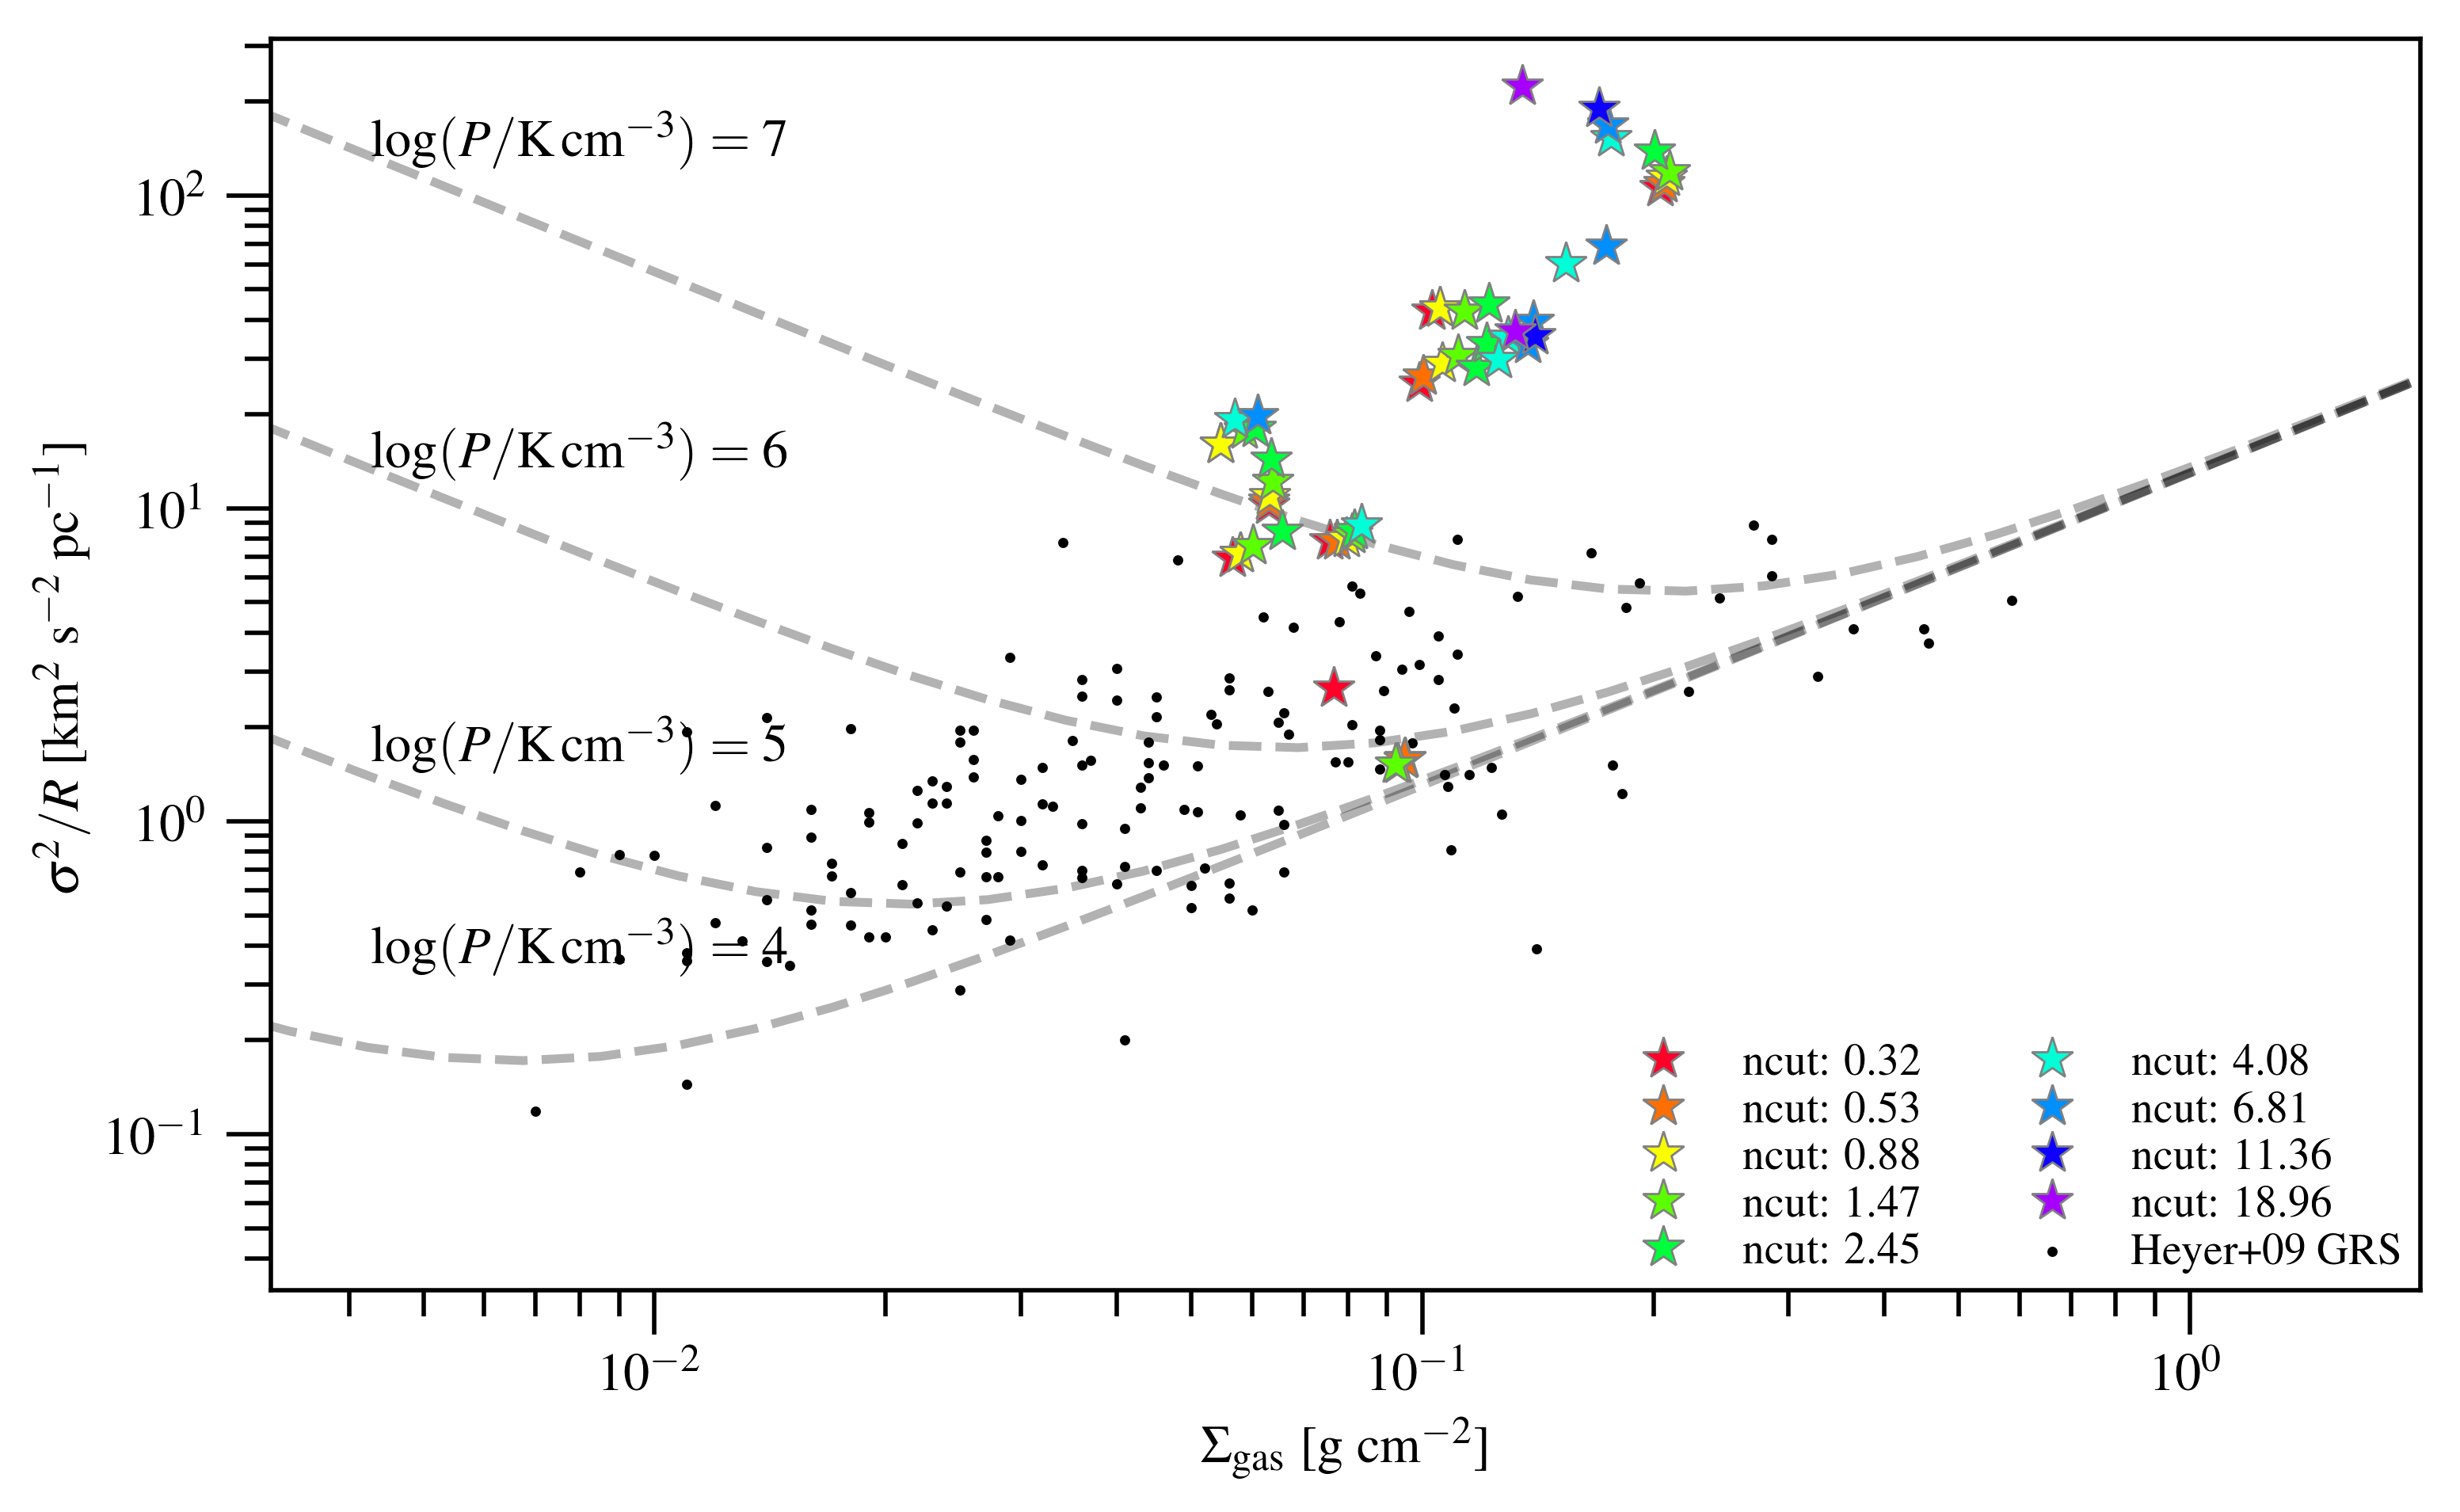
\includegraphics[trim=0 0 0 0, clip, width=0.65\textwidth]{\figpath/ss16_PVE.png}
%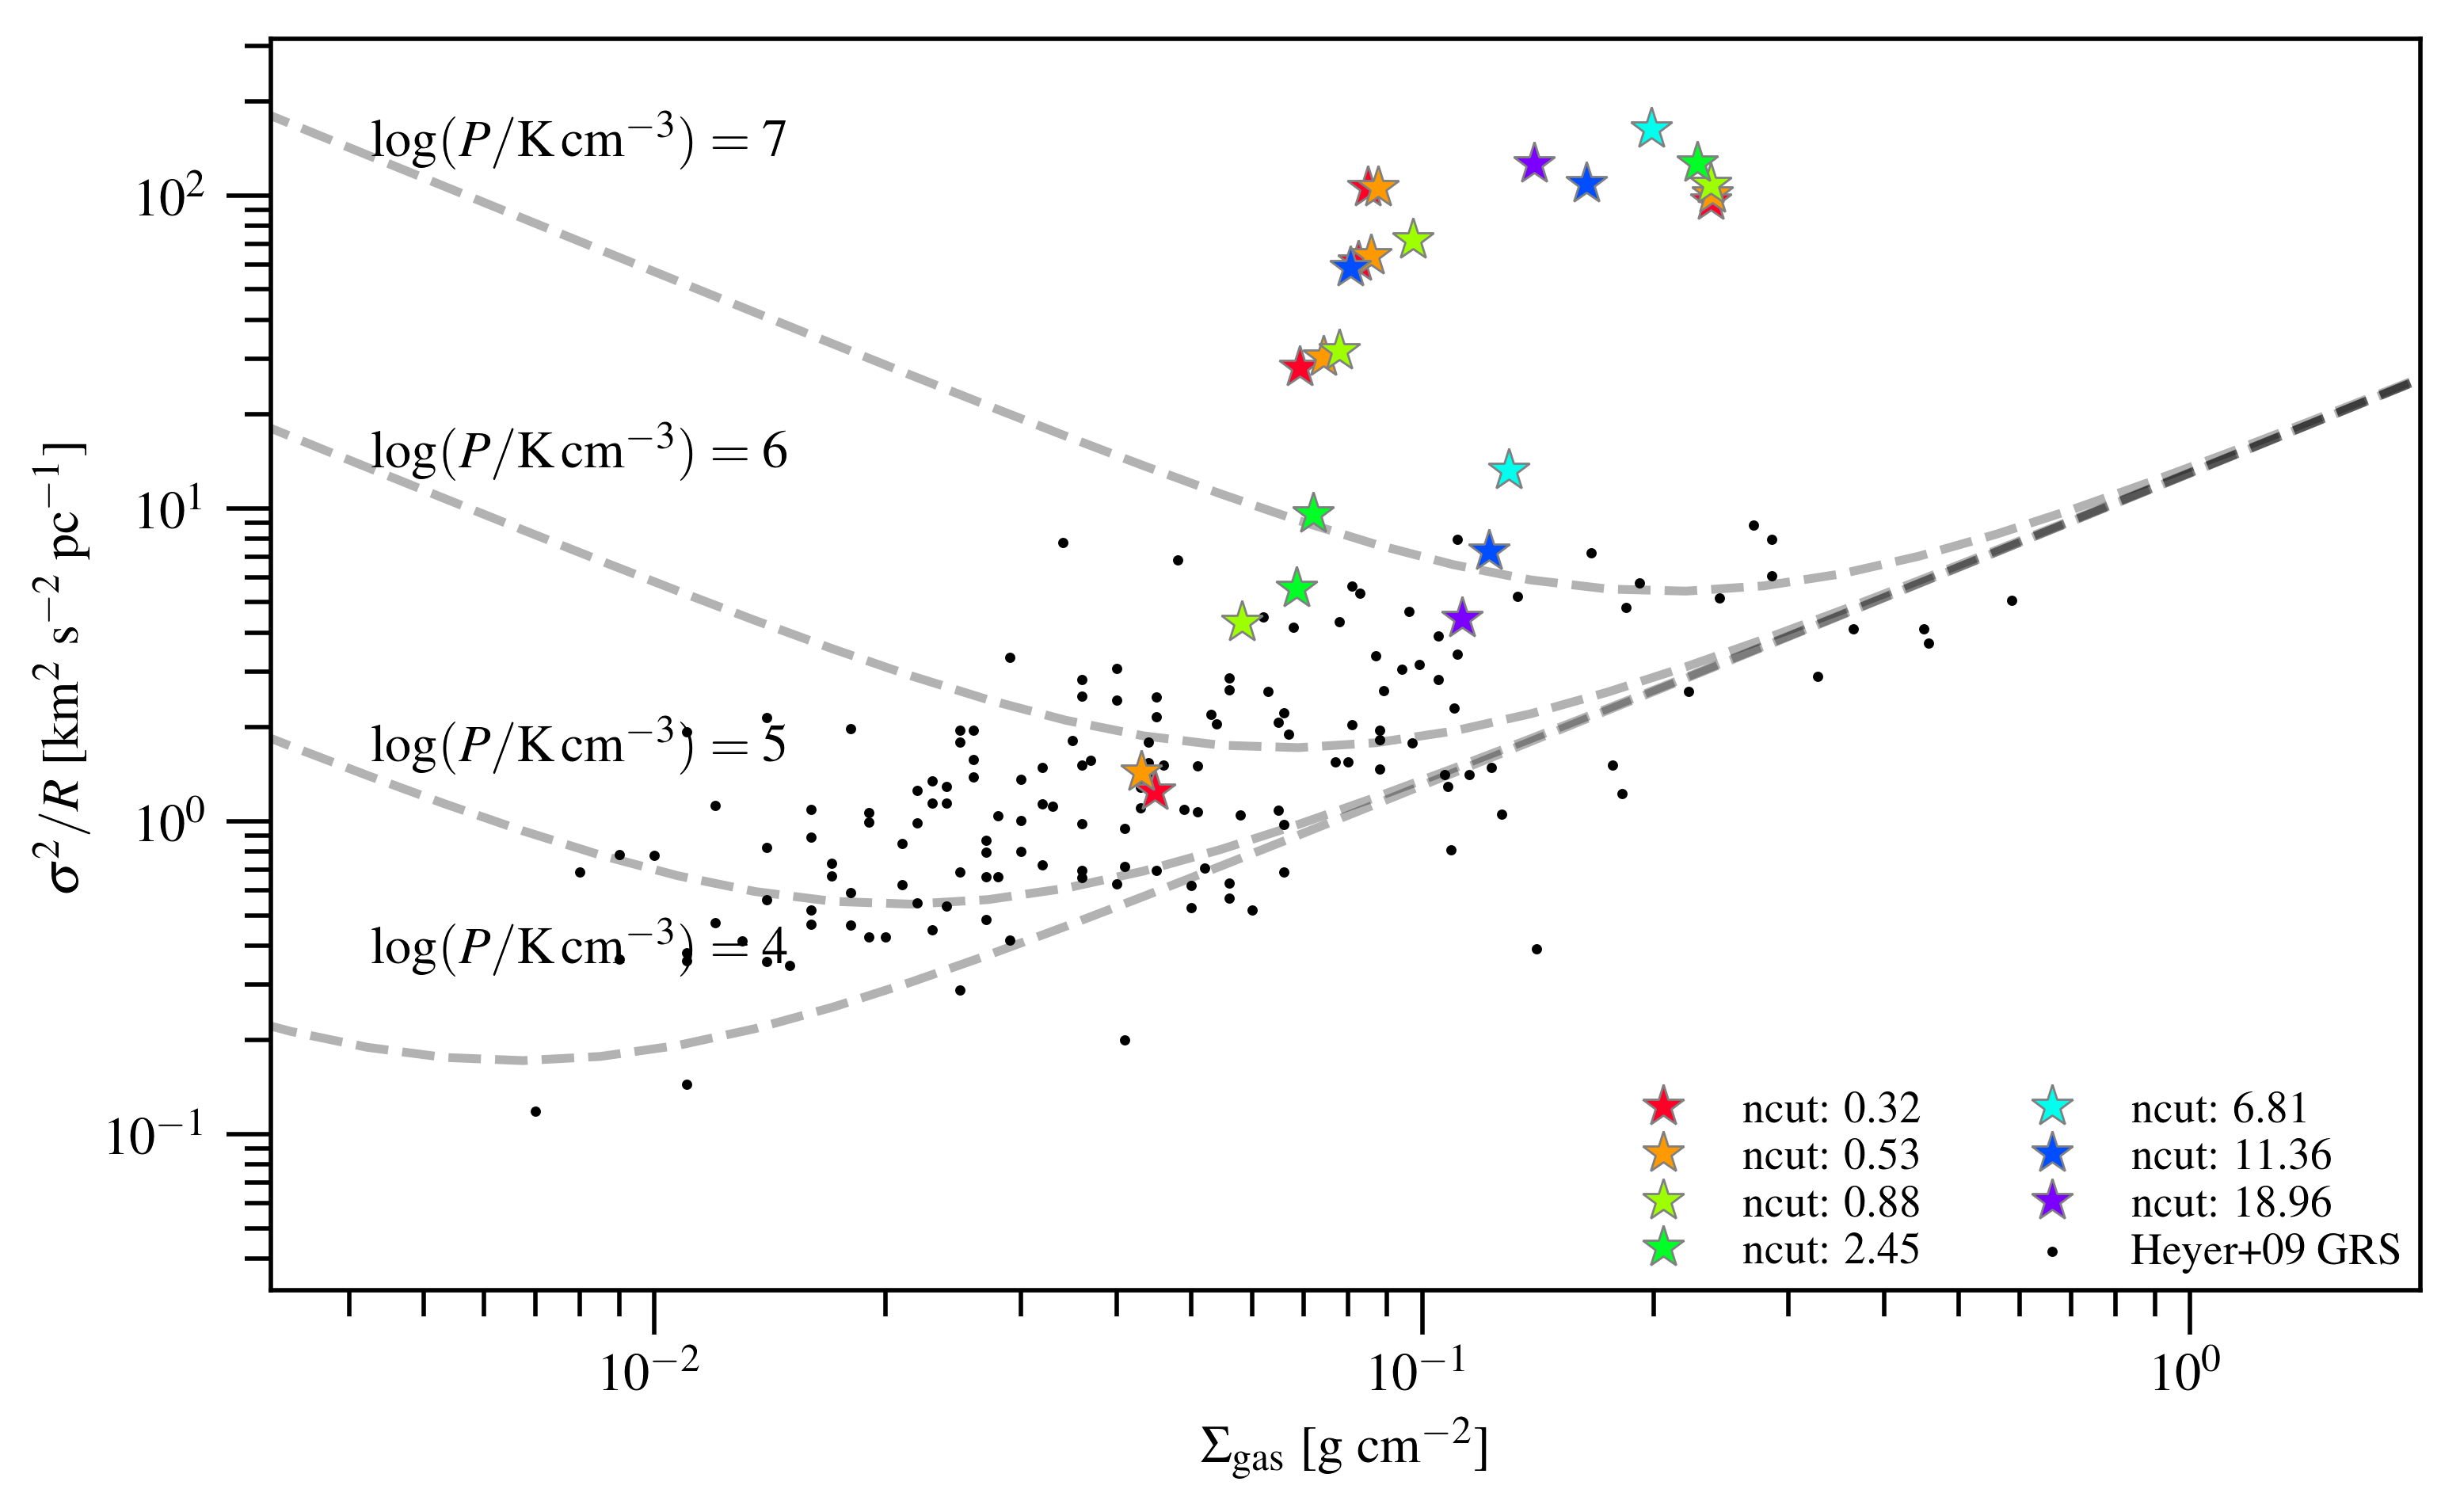
\includegraphics[trim=0 0 0 0, clip, width=0.65\textwidth]{\figpath/ss27_PVE.png}
%\caption{
%$\sigma^2/R - \Sigma_{\rm gas}$ relation of the MCCs identified in our simulation (star symbols)
%in the accretion phase (top panel) and the starburst phase (bottom panel)
%compared to those observed in the Milky Way (black dot markers; \citealt{Heyer09a}).
%The V-shaped dashed lines show the loci along which the given external pressures
%are needed for MCCs to have linewidth $\sigma$ for a given set of surface densities (see \Sec{PVE}).
%Similar to \Fig{alpha16}, star symbols are color-coded by $n_{\rm cut}$.
%Star symbols along the locus of $\log{(P/\textrm{K cm}^{-3}) = 6}$
%correspond to MCCs in the satellite galaxies.
%\label{fig:alpha27}}
%\end{figure*}
%\end{comment}

%
%\begin{comment}
%
%\begin{figure*}[htbp]
%\centering
%\includegraphics[trim=0 20 30 30, clip, width=0.7\textwidth]{\figpath/{ss16_gas_toomre_proj_0_zoom_2.0_kpc}.png}
%\caption{
%Maps of the total gas surface density (top left),
%velocity dispersion (top right),
%epicyclic frequency (bottom left),
%and Toomre $Q$ parameter (bottom right) in the $xy$-plane.
%Modest smoothing has been applied to the maps.
%A divergent colormap is used for the Toomre $Q$ map to facilitate
%identification of regions above and below $\log{Q_{\rm gas}}$\eq0.
%Crosses correspond to positions of MCCs identified using the lowest $n_{\rm cut}$. % using 0.32
%Positions of sub-MCCs are not shown (but see top row of \Fig{Qeff} for an example).
%\label{fig:Q}}
%\addtocounter{figure}{-1}
%\end{figure*}
%
%\begin{figure*}[htbp]
%\centering
%\includegraphics[trim=0 20 30 30, clip, width=0.7\textwidth]{\figpath/{ss16_gas_toomre_proj_1_zoom_2.0_kpc}.png}
%\caption{Continued. Maps showing the various quantities projected on the $xz$-plane.}
%\addtocounter{figure}{-1}
%\end{figure*}
%
%\begin{figure*}[htbp]
%\centering
%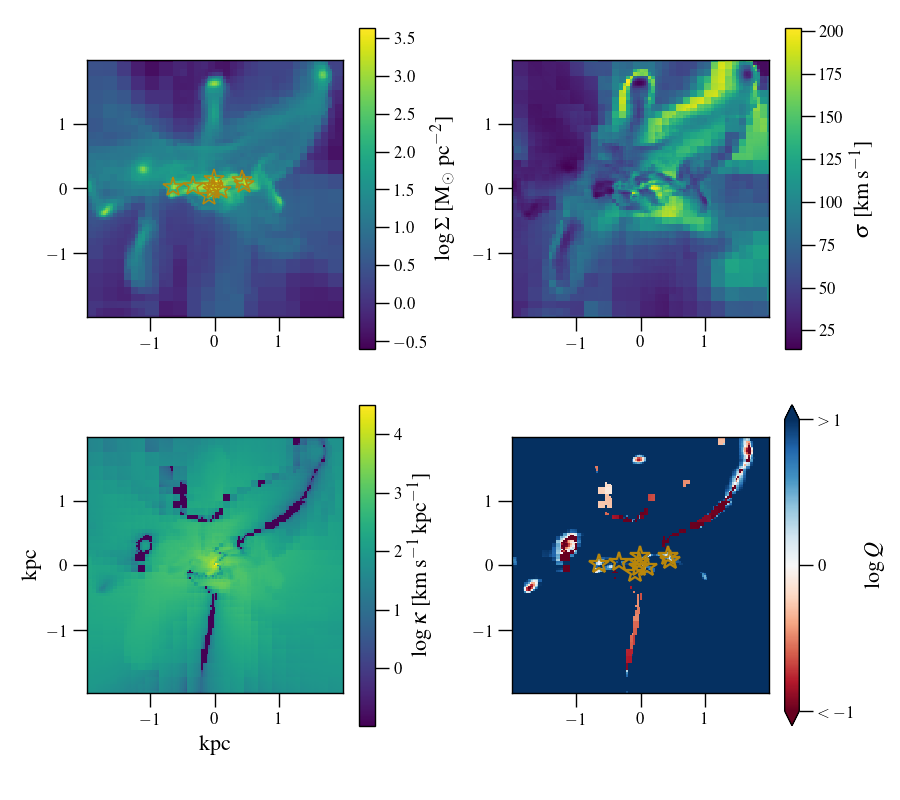
\includegraphics[trim=0 20 30 30, clip, width=0.7\textwidth]{{\figpath/ss16_gas_toomre_proj_2_zoom_2.0_kpc}.png}
%\caption{Continued. Maps show the various quantities projected on the $yz$-plane.}
%\end{figure*}
%
%\begin{figure*}[htbp]
%\centering
%\includegraphics[trim=0 20 30 30, clip, width=0.7\textwidth]{\figpath/{ss16_star_toomre_proj_0_zoom_2.0_kpc}.png}
%\caption{
%Same as \Fig{Q} but for the stellar component, projected in the $xy$-plane.
%\label{fig:Qstar}}
%% \addtocounter{figure}{-1}
%\end{figure*}
%
%\begin{figure*}[htbp]
%\centering
%\includegraphics[trim=10 0 100 20, clip, width=0.35\textwidth]{\figpath/{ss16_toomreEff_proj_0_zoom_2.0_kpc_0.32}.png}
%\includegraphics[trim=30 0 10 20, clip, width=0.425\textwidth]{\figpath/{ss16_toomreEff_proj_0_zoom_2.0_kpc_6.81}.png}  \\
%\includegraphics[trim=10 0 0 10, clip, width=0.425\textwidth]{\figpath/{ss16_gas_SD_proj_0_zoom_2.0_kpc}.png} \\
%\includegraphics[trim=30 25 30 20, clip, width=0.4\textwidth]{\figpath/{ss16_toomreEff_proj_0_zoom_0.8_kpc_6.81}.png}
%\includegraphics[trim=10 0 0 0, clip, width=0.38\textwidth]{\figpath/{ss16_gas_SD_proj_0_zoom_0.8_kpc}.png}
%\caption{
%Effective two-component Toomre $Q_{\rm eff}$ (top row)
%and gas surface density (middle) maps projected onto the $xy$-plane.
%Positions of MCCs identified using the lowest $n_{\rm cut}$\eq0.32\,cm$^{-3}$ (top left; same as \Fig{Q})
%and $n_{\rm cut}$\eq6.81\,cm$^{-3}$ (top right) are overplotted as crosses.
%Bottom row: Effective $Q_{\rm eff}$ (left) and gas surface density (right) maps zoomed in on the central 1.5\,kpc region.
%Cross markers indicate positions of MCCs identified with $n_{\rm cut}$\eq6.81\,cm$^{-3}$ (same as top right).
%Modest smoothing has been applied to the maps.
%A divergent colormap is used for the Toomre $Q$ map to facilitate
%identification of regions above and below $\log{Q_{\rm gas}}$\eq0.
%Some MCCs lie in regions of $\log{Q_{\rm eff}}\gtrsim0$, whereas regions of $\log{Q_{\rm eff}}\lesssim0$
%are likely gravitationally unstable.
%\label{fig:Qeff}}
%% \addtocounter{figure}{-1}
%\end{figure*}
%%\clearpage
%
%\end{comment}

%--------------------------------------------------------------------------
%                                Discussion
%--------------------------------------------------------------------------
\section{Discussions and Implications}\label{sec:diss}

\subsection{Placing Results in the Context of Existing Observations} \label{sec:diss1}

The MCCs of \flower has dynamics largely similar to those observed in $z$\ssim2 spatially resolved studies of gas-rich star-forming galaxies, in terms of their velocity dispersions, sizes, and gas surface densities (\Fig{larsons_single}; see e.g., \citealt{Swinbank11a}), with sizes of the order of $R\simeq$\,100\,pc and velocity dispersions of $\sigma\simeq$\,20$-$80\,\kms.
%
% velocity dispersion, larsons
%
Their velocity dispersions are also comparable to those observed in the inner Milky way and nearby gas-rich galaxies (e.g., M64; \citealt{Oka01a, Rosolowsky05a, Heyer09a}), which lies along the locus of $\sigma\propto R^{0.56}$. Such high velocity dispersions and surface densities are expected since they are located in the nuclear regions of the galaxy, where the potential well is also deep. The higher velocity dispersions
(see footnote~\ref{ftn:veldisp} on page \pageref{ftn:veldisp}) of these MCCs can also be understood as they have experienced more recent episodes of \SF as \flower is assembling its stellar mass (these MCCs also have higher stellar-to-gas mass ratios of $\sim$60).
%
In fact, by the accretion stage (see \Fig{SFH}a) at $z\simeq$\,7.2, 
\flower has assembled a stellar mass of $M_\star$\eq7.5\E{9}\,\Msun. Thus, the higher velocity dispersion is due in part to the stronger stellar feedback compared to e.g., MCCs in its satellites ($\sigma\approx$10\,\kms).


The high pressure observed in \flower is comparable to what has been observed in local ultra-luminous IR galaxies (ULIRGs); however, the molecular clouds in the latter are concentrated within their central regions and have typical sizes of $\sim$70-100\,pc and masses on the order of $\sim$10$^9$\,\Msun \citep{Downes98a, Sakamoto08a}. In our simulated galaxy, the high pressure MCCs of \flower are found throughout the disk. This difference likely stems from the different physical mechanisms giving rise to the formation (and thus the nature) of these molecular structures.
%
For instance, in local ULIRGs, they are likely form by shock compression and cloud-cloud collision after large amount of gas from the pair of progenitor galaxies are being funneled toward the central region \citep{Tan00a, Wu18a}.
% Tasker09a
On the other hand, the highly turbulent structures of \flower likely result from 
extra-planar flows that are due to gas accretion onto the galaxy and SN-driven outflows \citep{gallerani:2018,kohandel:2019}.
The presence of such extra-planar flows may also be the 
dominant mode for forming the highly supersonic massive MCCs observed in gas-rich star-forming galaxies at $z$\ssim2 (see also e.g., \citealt{Swinbank11a}) --- but the observed size scales could also result from resolution limit where the true physical scales of MCCs in $z$\,\ssim2 galaxies could be smaller in reality.
%
The constant inter-cloud collision as gas is being accreted onto the main galaxy would also render
the MCCs to be gravitationally unbound (see e.g., \citealt{Dobbs11a}), which is
consistent with the high $\alpha_{\rm vir}$ found for the MCCs in the main disk of \flower.

% mass-size relation
MCCs of \flower lie below the locus of $A_V$\eq100\,mag followed by Milky Way clouds in the mass-size relation shown in \Fig{MR}. This can be understood by acknowledging the fact that a H$_2$ molecular cloud does not necessary contain CO (e.g., as CO forms deeper in molecular clouds), and that our simulation does not have enough resolution to directly form CO\footnote{In fact, to form CO and make predictions for CO line emission in the work presented by \citet{Vallini18a}, we model the internal structure of MCC within each cell in our simulation.}.
%
That is, the MCCs of \flower lying along the locus of $A_V$\eq4\,mag likely manifests from the fact that the MCCs in our simulation have lower column densities than the star-forming cores observed in the Milky Way, which are observationally well-resolved within an MCC, and indeed, have sufficient column density to form CO.

The \citet{Kauffmann10c} relation suggests that regions with high-mass \SF follow 
an ``internal'' mass-size relation where $M\propto R^{1.33}$.
If this holds for MCCs of \flower, an extrapolation of the \citet{Kauffmann10c} relation down to $\sim$1\,pc would correspond to structures with masses and sizes comparable to those of the cores found in
regions of high-mass \SF. That is, the MCCs identified have mass-size relations suggesting they are capable of high-mass \SF. 

% different evolutionary stages
In the scaling relations examined, we find similar MCC properties in relation to those observed in the nearby Universe between the accretion phase and the starburst phase of \flower (see \Fig{larsons_single}). That is, we do not find any quantitative major differences in the MCC properties between the accretion and the starburst phase, which are separated by $\simeq$300\,Myr. \DL{some MCCs in SB phase have
lower $\alpha_{\rm vir}$ and pressure, but 
is there any significance in that?}

\subsection{Origin and Physical Scales of MCCs} \label{sec:origin}

The largest molecular structure identified is essentially the main disk of \flower and breaks down into smaller substructures that are denser as we increase $n_{\rm cut}$ (see e.g., \Fig{alpha16-28}). Overall, the MCCs we identified are much bigger in size and mass than nearby GMCCs, but comparable to those observed in $z$\,\ssim2$-$4 galaxies based on spatially resolved imaging \citep{Swinbank11a}.

% mass scale
Observations of nearby gas-rich galaxies such as M64 and NGC\,253 show higher velocity dispersions compared to the disk/mid-plane of the Milky Way but consistent with those observed in the inner regions of Milky Way and M51 \citep{Oka01a, Rosolowsky05a, Heyer09a, Hughes13b, Leroy15a, Rice16a}.  % also higher $P_{\rm int}$,
% which is $\propto\rho\sigma^2$
% M51: Colombo+14
However, clouds in nearby gas-rich galaxies are bigger in size (approximately an order of magnitude) and mass (approximately two orders of magnitude).
These bigger clouds have been interpreted as a result of their higher gas mass fractions, surface densities, and velocity dispersions,
since fragmentation occurs near the Jeans length $L_J\propto\sigma^2/\Sigma$ and
Jeans mass $M_J\propto\sigma^4/\Sigma$ for dispersion-supported structures.

Based on the scaling of $M_J$\eq$\sigma^4/(G^2\Sigma)$ for the Jeans mass, a
velocity dispersion of $\sigma\approx50$\,\kms and a
gas mass surface density of $\Sigma_{\rm gas}\approx450$\,\Msun\,pc$^{-2}$ yields
$M_J\sim$\,8\E{8}\,\Msun, which is in good agreement with the mass range found in the MCCs identified (see \Fig{dist}).
%
Similarly massive molecular clouds have been reported in idealized closed-box isolated galaxy simulations done at higher resolution (e.g., a maximum
resolution of 3\,pc in the 48\,kpc box studied by \citealt{Behrendt16a}).
Note, however, that the IGM and merger and accretion histories are not properly modeled in such simulations since they adopt non-cosmological initial conditions. That said, this is reassuring --- our results are not far off in spite of the limited resolution ($l_{\rm cell}\approx$\,30\,pc).

%Note that regions of $Q\lesssim1$ is actually somewhat
%less than the number of MCCs we have identified based on density threshold ---
%but this has something to do with the dependence on
%$n_{\rm cut}$. The number of MCCs and regions of low $Q$ are comparable if we only look at
%MCCs identified at the highest $n_{\rm cut}$.

% alpha parameters
As shown in \Fig{larsons_single},
the virial parameter of the sub-MCCs is about $\alpha_{\rm vir}\gtrsim10$, which is considerably lower than their ``parent'' MCCs found in the main disk of \flower ($\alpha_{\rm vir}\gtrsim100$).
%
For the MCCs in the satellite galaxies, a lower virial parameter is found compared to the (sub-)MCCs in the main disk of \flower, with $\alpha_{\rm vir}\approx$\,2.
Differences in their $\alpha_{\rm vir}$ most likely result from the weaker stellar feedback in the satellites as they have experienced less episodes of \SF compared to \flower (i.e., lower stellar-to-gas mass ratios of $\sim$0.1).

% pext
As shown in \Fig{larsons_single},
MCCs in the main disk of \flower have higher pressure than the sub-MCCs. The lower virial parameter and external pressure of the sub-MCCs compared to their parent MCCs are consistent with the notion that collapsing structures result from local gravitational instability within globally non-collapsing structures \citep[see e.g.,][]{Ballesteros-Paredes11a}, which are supported by turbulence and rotation on large scales.
%Based on the virial parameter, velocity dispersion, and pressure of the MCC identified in the main disk of \flower,
%the MCC itself is gravitationally unbound and supported by turbulence (from the feedback of multiple episodes of \SF)
%and galactic rotation on large scales.
%% Turbulence in these substructures further dissipates in % e.g., shocks on even smaller scales, allowing sub-MCCs to be bound and collapse.

For MCCs in the satellite galaxies, we find even lower pressures and virial parameters, which are comparable to those found in clouds formed in the galactic disks  ($\alpha_{\rm vir}$\eq0.2$-$10; \citealt{Dobbs08a, Tasker09a}).
This suggests that MCCs identified in the satellite galaxies are likely to be collapsing structures, and thus, \SF is expected to continue as gas from satellite galaxies is being accreted onto the main galaxies during the EoR.

\subsection{Stability of MCCs}


\begin{figure*}
\centering
\includegraphics[width=0.9\textwidth]{\figpath/{ss16_toomre_combined_2by2_0_2.0}.pdf}
\caption{
Surface density maps of the gas (top left) and stellar (top right) components of \flower and
their radial velocity dispersion maps projected onto the $xy$-plane.
%
\label{fig:sigma}}
\end{figure*}

\begin{figure*}
\centering
\includegraphics[trim=0 0 0 0, clip, width=0.92\textwidth]{\figpath/{ss16_toomre_combined_3by1_0_2.0}.pdf}
\includegraphics[trim=0 0 0 65, clip, width=0.95\textwidth]{\figpath/{ss16_toomre_combined_3by1_0_0.8}.pdf}
\caption{
Toomre $Q$ maps derived from the
central $r$\eq2\,kpc (top row) and $r$\eq0.8\,kpc (bottom row) of \flower.
Gas-only $Q_{\rm gas}$ are shown in the left panels and stellar-only $Q_\star$ are shown in the middle panels.
Maps of the effective two-component Toomre $Q_{\rm eff}$ parameter are shown in the right panels.
All maps are projected onto the $xy$-plane.
Positions of MCCs identified with $n_{\rm cut}$\eq6.81\,cm$^{-3}$ are overplotted as star symbols.
A smoothing length of 30\,pc has been applied to the maps.
A divergent colormap is used for the Toomre $Q$ maps to facilitate
identification of regions above and below $\log{Q}$\eq0.
Some MCCs lie in regions of $\log{Q_{\rm eff}}\gtrsim0$, where regions of $\log{Q_{\rm eff}}\lesssim0$
are likely gravitationally unstable.
Close resemblance of the $Q_\star$ and $Q_{\rm eff}$ maps in the central region of \flower 
indicates that stellar component plays an important role in governing the stability of the MCCs against $m=0$  perturbations, highlighting the importance of accounting for stellar contribution when examining the stability of molecular gas in relatively evolved and enriched systems at high redshifts.
\label{fig:Qeff}}
\end{figure*}


Maps of the Toomre $Q$ parameters for the gas, stars, and the effective two-component $Q_{\rm eff}$ are shown in \Fig{Qeff}
(see also \Fig{h2density} for example of MCCs identified in this evolutionary stage of \flower
using different $n_{\rm cut}$). 

Close resemblance of the $Q_{\rm eff}$ and $Q_{\star}$ maps indicates that contributions from the stellar component play an important role in governing the stability of the MCCs against $m$\eq0 perturbations. This can be understood since stars in \flower dominates the central part of the galaxy in mass, so their gravitational potential provides a non-negligible contribution to the instability.

Similarly, contribution from the thickness of the disk is important in \flower since its disk warped and cannot be considered thin, i.e., 
it has a scale height to radius ratio of $h/r_{\rm gal}$\ssim150\,pc/1\,kpc\,$\simeq$\,0.15.

That is, some MCCs are found in regions of $Q_{\rm gas}$\ssim1, consistent with the expectation that they correspond to regions of high surface densities that are gravitationally unstable. 
Note, however, that when including the stabilizing effects due to the stellar potential of \flower and the
thickness of its disk (via $\sigma_z$), some of these MCCs are consistent with  $Q_{\rm eff} > 1$. 
This demonstrates the importance of accounting for stellar contribution and disk thickness 
when examining the stability of molecular gas structures.
This consideration is especially relevant for the relatively evolved and enriched systems at high-$z$, 
that are preferentially being imaged at high resolution with ALMA.
In the outer regions of \flower, on the other hand, $Q_{\rm eff}$ resembles $Q_{\rm gas}$, with 
both $\log{Q_{\rm gas}}$ and $\log{Q_{\rm eff}} < -1$. 
Notably, these are the more gas-rich regions (see \Fig{sigma}).

The apparently large virial parameters seen in the MCCs of \flower can be understood using the Toomre $Q$ parameter (see \Fig{Qeff}). We first note that fragmentation {\it can} happen in regions of low $Q$ (if we only consider instability against axisymmetric perturbations), but further evolution/collapse depends on the dynamics or equation of state of the gas.
%
Such fragmentation is expected to take place at the critical scale length $\lambda_{\rm crit} < 2 \pi^2 G \Sigma / \kappa^2$. Second, this fragmentation scale is greater than the typical size of GMCCs. This could be interpreted as a result of instability setting the scales for fragmentation, but the star-forming GMCCs correspond to the collapsing, denser, and cooler molecular structures that are on smaller scales.
%
Thus, the high virial parameter found for most MCCs in \flower, which is the ratio between the velocity dispersion (accounts for effect of pressure and rotation) and surface density, indicate that most of them are not collapsing structures. As such, 
some MCCs are found to lie in regions of $Q_{\rm eff}>1$.
% some MCCs at Q < 1, some are marginally stable against m=0 mode perturb, some are Q>1.
Only in (the denser) regions with a low Toomre $Q_{\rm eff}$ parameter and when the cooling time is lower then the dynamical time star formation can proceed in {\it clumps} and {\it cores} with low virial parameters.

Note that even in stages when \flower~is star forming we find that most of its MCCs have high $\alpha_{\rm vir}$. This seem to be self-contradictory: if most of the molecular gas in \flower are stable against collapse, how does it sustain its high SFR of $\sim$70\,\Msun\,yr\pmOne in the starburst phase? Such tension in the interpretation is understood as follows.
%
First, our results are limited by the resolution of the simulation, i.e., in \flower~we do not resolve \SF in {\it cores} and {\it clumps} as in the classical molecular cloud hierarchy. This re-iterates the statement about low $Q$ above.
%
Second, due to turbulence dissipation on small-scales, such (sub-)structures are no longer supported by large-scale gravitational potential and differential rotation. This in turn enables sub-regions of the MCCs to collapse and potentially form OB associations out of these unbound MCCs \citep{Clark04a, Clark05a}.
%
Further, mechanisms causing non-axisymmetric perturbations (e.g., arms) to the gravitational potential can induce orbit crossing, shocks and dissipation in gas, promoting turbulence dissipation and collapse on smaller scales to trigger \SF. These mechanisms are likely important given high $Q_{\rm eff}$ found across \flower and its few tens of solar masses per year SFR, albeit sporadic.
Finally, the SFR of \flower is very bursty and high SFR stages are only transient.
% the giant MCCs found are likely due to non-axisymmetric mode.

%--------------------------------------------------------------------------
%                                Conclusions
%--------------------------------------------------------------------------
\section{Summary}      \label{sec:conclusion}

We study the dynamical properties of molecular clouds complexes and their temporal evolution in a \z$\sim$\,6 prototypical galaxy, \flower,
at the EoR using state-of-the-art cosmological zoom-in simulation (\ncode{Serra}),
which includes a chemical network to determine the formation of molecular
hydrogen, heating and cooling of the ISM by metals, and detailed stellar feedback.
We use a clump-finding algorithm and a set of H$_2$ volumetric densities
to identify MCCs and their sub-structures in \flower and its satellites.
We decompose the molecular structures into non-overlapping tiles
by identifying a set of different density contours at different evolutionary stages.
Such identification method is similar to MCC identification based on 
contour levels/surfaces of surface brightness maps/cubes of molecular line tracers (e.g., CO, CS, NH$_3$),
since the line luminosity scales with the molecular gas density (modulo optical depth effects).

We extract properties such as mass, size, Mach number, velocity dispersion, gas surface density, and virial parameter for each MCC and we perform a Toomre-$Q$ stability analysis. The properties of the MCCs in \flower are compared with observed MCCs in the Milky Way disk, the Galactic center, and gas-rich starburst galaxies in the local Universe and at the peak epoch of cosmic \SF. This is done for different evolutionary stages of \flower.

We find that the MCC of \flower are highly supersonic, with high velocity dispersions ($\sigma\approx$\,200\,\kms) comparable to
those observed in $z$\ssim2 starburst galaxies.
The mass scale of the MCCs is of the order of $10^{5.5-8.5}$\,\Msun, depending on the chosen H$_{2}$ cut. 
The $\sim$200\,pc-scale MCCs found with a low density threshold
correspond to the arms of the disk of \flower which break down into smaller $\lesssim$100\,pc-scale MCCs at higher density thresholds.
The more massive and bigger MCCs in \flower compared to the Milky Way
likely result from the higher gas mass fraction, surface density, and velocity dispersion,
which set the scale for fragmentation.
This physical scale is
consistent with what has been found in higher resolution idealized simulation of isolated galaxies.
Our simulation here confirms these results at EoR and under
the influence of continuous gas accretion from the surrounding IGM (see e.g., \citealt{Klessen10a, Goldbaum11a}).

We compare the dynamics of MCCs in \flower to \obs in the context of the Larson's relation.
The MCCs of \flower are found to have higher $\sigma$ and $\Sigma$ systematically regardless of the
density threshold $n_{\rm cut}$ adopted in identifying the structures.
 The found scaling relations are insensitive to the various density cuts. 
 The velocity dispersion remains $\gtrsim$100\,\kms even when we increase the density threshold and 
 even for the molecular substructures. 
 Such a high velocity dispersion likely results from the strong supernova and stellar feedback \flower experienced 
 over the multiple episodes of bursty \SF.

Virial analysis indicates that MCC/arms of the main disk of \flower are unbound, but substructures have
lower virial parameter. Some of these sub-MCCs have Toomre $Q_{\rm eff}$ parameters consistent with being
gravitationally unstable. This is consistent with the notion that collapsing structures resulting from
gravitational instability occur within globally stable structures, which are
supported by turbulence and rotation on large scale.
We also find $\alpha_{\rm vir}\approx$\,2 for MCCs in the satellite galaxies, which we interpret as
result of the weaker/delayed stellar feedback compared to \flower. 
In particular, some of the MCCs in the satellites are collapsing structures that have not yet formed stars, as confirmed by their
higher gas-to-stellar fractions.
In terms of the scaling relations examined, we do not observe any significant
temporal variations in the MCC dynamics over the course of 700\,Myr traced in our simulation.

Determining the multi-phase ISM properties of early galaxies
is a critical piece to understanding the evolution and
assembly history of galaxies, since they set the pace
for chemical reactions and excitation rates for the coolants in the ISM (and subsequent star formation).
Observations leveraging the combination of spatial-spectral imaging of
multi-band continuum and spectral line emission are crucial for better understanding
the role of \highz galaxy populations
in the context of galaxy evolution and the ISM physics behind their intense star formation in the early Universe.
Cosmological zoom-in simulations, such as \ncode{Serra}, while inherently limited in galaxy
statistics and is subject to the sub-grid models adopted,
serve as an useful avenue/tool for examining and making predictions on the morphology and dynamics of
the molecular ISM of the first galaxies.
%Future higher resolution zoom-in simulations would certainly be useful to understand
%the evolving dynamical properties of the lower-mass molecular structures in
%galaxies at EoR under the influence of gas inflow/outflow (i.e., accounting for energy injection at large scale due to infall/outflow).
These predictions can in turn be
tested with high resolution imaging of the gas content in the first galaxies with telescopes such as ALMA and the ngVLA, thereby
enabling us to test our findings and refine future simulations to shed light on the physical processes behind
\SF since the cosmic dark ages.


%==============================================================================
%                                Back matters
%==============================================================================
% ACKNOWLEDGEMENTS
%-------------------------------------
\acknowledgements

We thank Jens Kauffmann, Thushara Pillai, and Mark Swinbank for sharing their data, and Jens for useful discussions.
%
TKDL acknowledges support by the NSF through award SOSPA4-009 from the NRAO and support from the Simons Foundation.
%
AF acknowledges support from the ERC Advanced Grant INTERSTELLAR H2020/740120.
%
This work is based on a project developed at the Kavli Summer Program in Astrophysics (KSPA) held at the Center for Computational Astrophysics of the Flatiron Institute in 2018. The program was co-funded by the Kavli Foundation and the Simons Foundation.
%
We thank the KSPA Scientific and Local Organizing Committees, and the program founder, Pascale Garaud, for supporting the genesis of this work.
%
We also thank the Center for Cosmology and Particle Physics at the New York University for their hospitality in hosting us after the steam pipe explosion in NYC during the KSPA.
%
This research has made use of NASA's Astrophysics Data System Bibliographic Services.
%
We acknowledge use of the Python programming language \citep{VanRossum1991}, Astropy \citep{astropy}, Cython \citep{behnel2010cython}, Matplotlib \citep{Hunter2007}, NumPy \citep{VanDerWalt2011}, \ncode{Pymses} \citep{Labadens2012}, SciPy \citep{scipyref}, and \ncode{yt} \citep{Smith09a,Turk11a}.
%
%and \ncode{yt}, a community-developed Python package for analyzing simulation data in Astronomy.

\bibliographystyle{yahapj}
\bibliography{master_cleanup,codes}

\begin{comment}
\appendix
\section{Variation in MCC Properties Depending on the Choice of Density Cuts and Temporal Evolution in Cloud Dynamics}    \label{sec:ncut}
% single Snapshot
We investigate possible variations in the dynamics of the molecular structures of \flower and its satellites to test the robustness of our results against the choice of density threshold by adopting
different sets of $n_{\rm cut}$ in identifying the MCCs.
That is, how sensitive are the structure properties, and thus, the results presented in \Sec{singless} dependent on the choice of density thresholds. We vary the choice of H$_2$ density for each of the evolutionary stages and find no obvious differences in our results (i.e., inferences on the dynamics of \z$\sim$\,6 MCCs in relation to those observed in nearby and \z$\sim$2 galaxies in the context of
cloud scaling relations).
%
In addition, for the densest MCC in the main disk of \flower, we find that while its size decreases as we increase $n_{\rm cut}$ --- as one would intuitively expect, the velocity dispersion remain approximately $\sigma\simeq$\,200\,\kms (see also \Fig{larsons_single}).
%
This lack of variation is reassuring, in the sense that at least on the scales studied here, the dynamics of the MCCs are not artifacts or biased by our choice of $n_{\rm cut}$. Our results are therefore robust to the various density cuts of choice.

% temporal evolution in Cloud Dynamics
We show the properties of all MCCs identified across all evolutionary stages in \Fig{larsons16-28} and \Fig{alpha16-28}. We find no quantitative differences in the cloud properties over the 700\,Myr traced in our simulation.

% -------------- all snapshots -----------


\begin{figure*}[htbp]
\centering
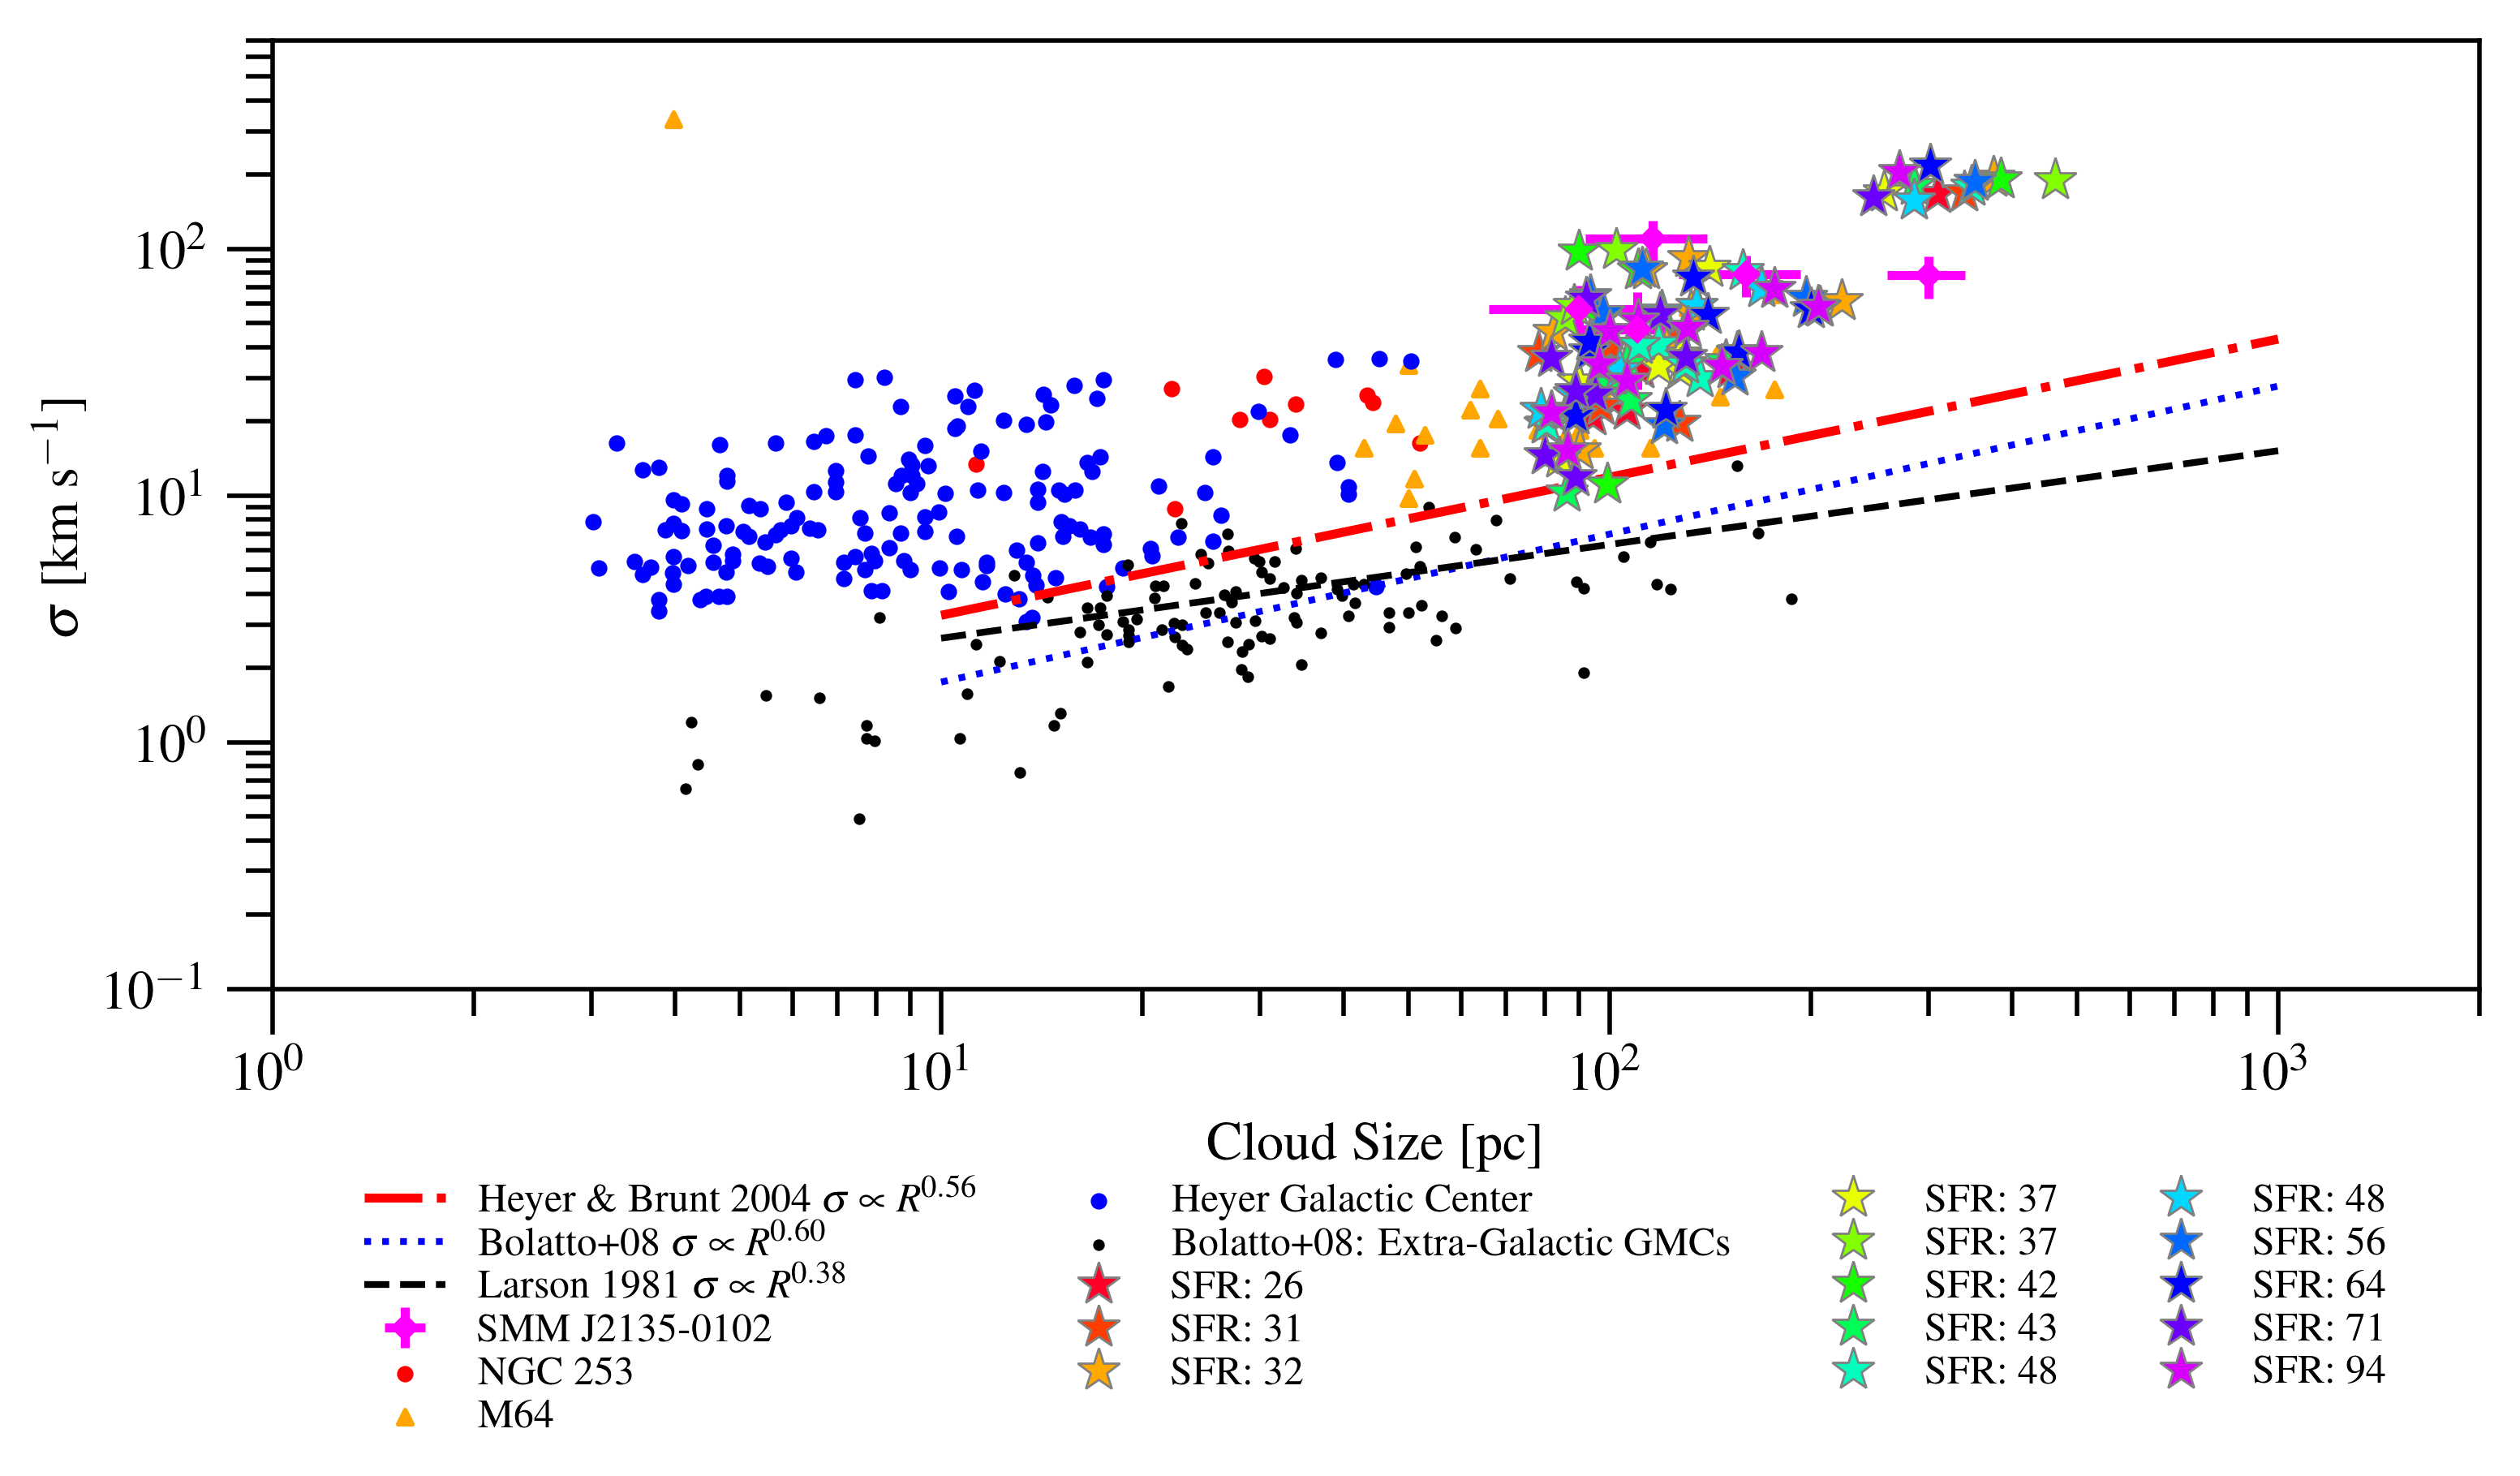
\includegraphics[trim=0 100 0 0, clip, width=0.85\textwidth]{\figpath/ss16-28_larsons.png}
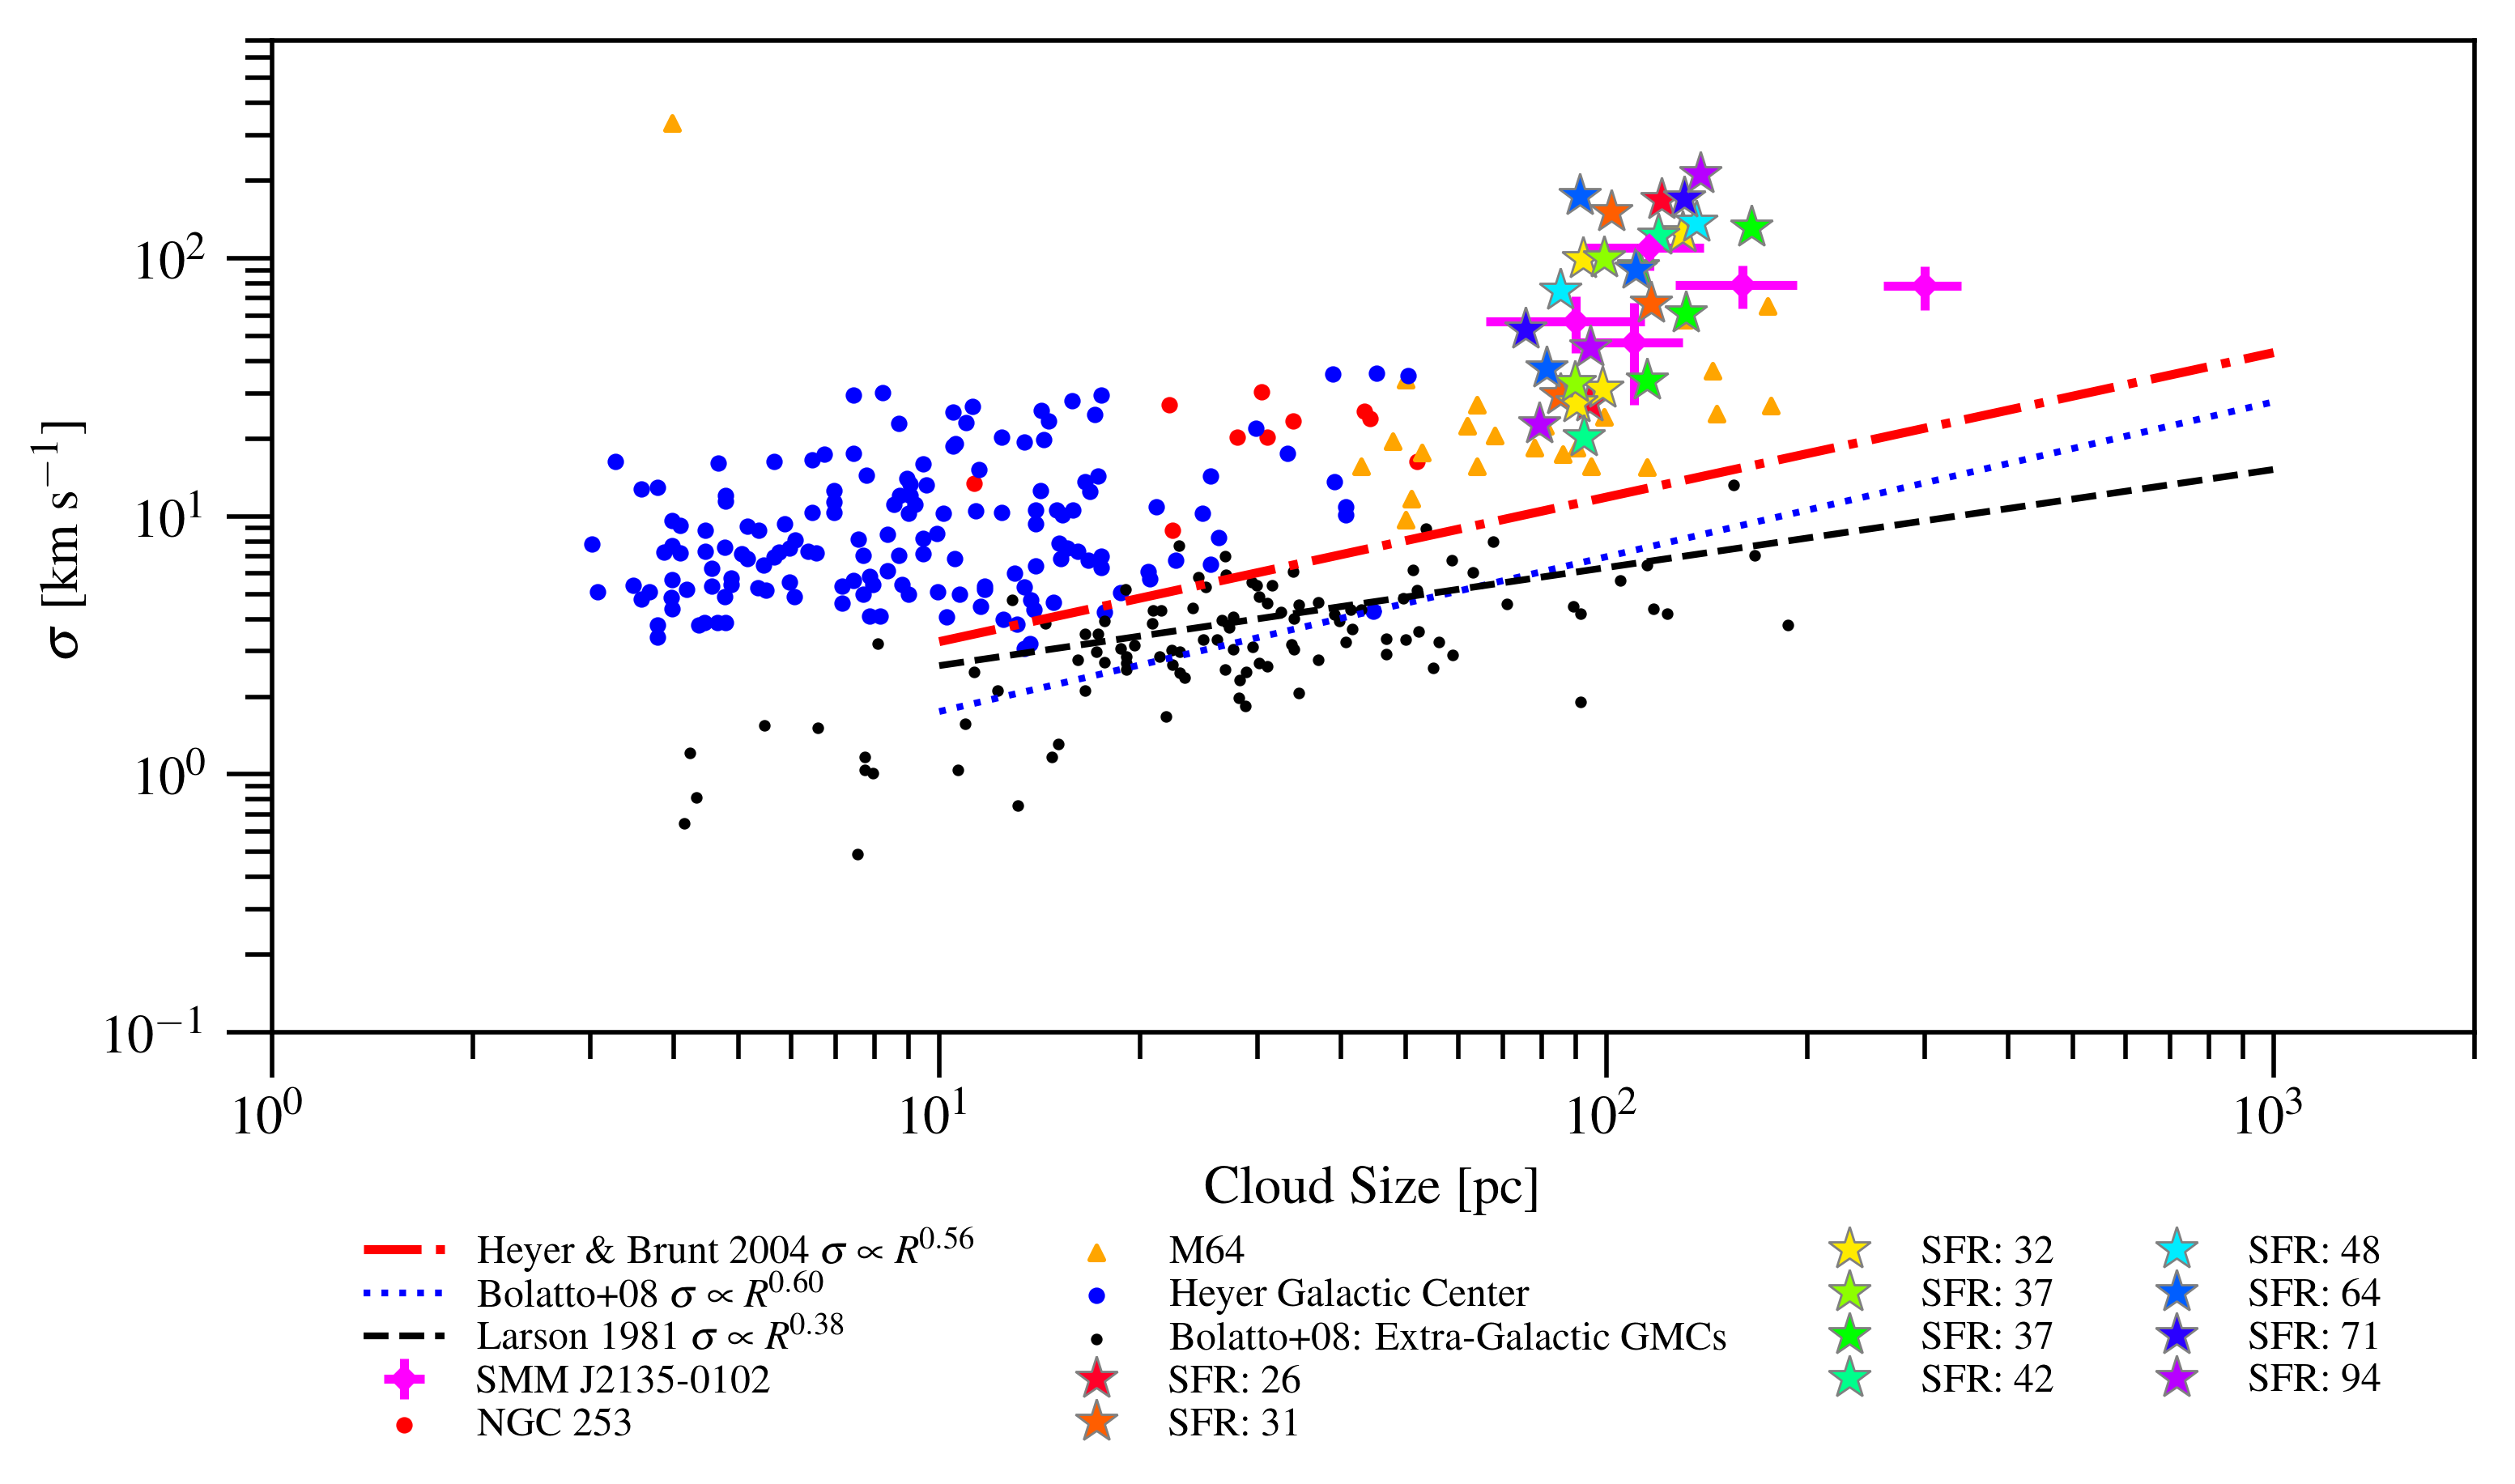
\includegraphics[trim=0 0 0 0, clip, width=0.85\textwidth]{\figpath/ss16-28-larsons-highncut.png}
\caption{
%Comparison of MCCs identified across all evolutionary stages (over 700\,Myr; star symbols)
to those observed in nearby and \z$\sim$2 star-forming galaxies
in the context of the linewidth-size relation.
%Bottom panel corresponds to including only the denser substructures/sub-MCCs identified in \flower
(i.e., MCCs here are identified with the highest $n_{\rm cut}$, see \Sec{method}).
By and large, we find no quantitative differences in the mass-size relation over the 700\,Myr traced in the simulation.
\label{fig:larsons16-28}}
\end{figure*}

\begin{figure*}[htbp]
\centering
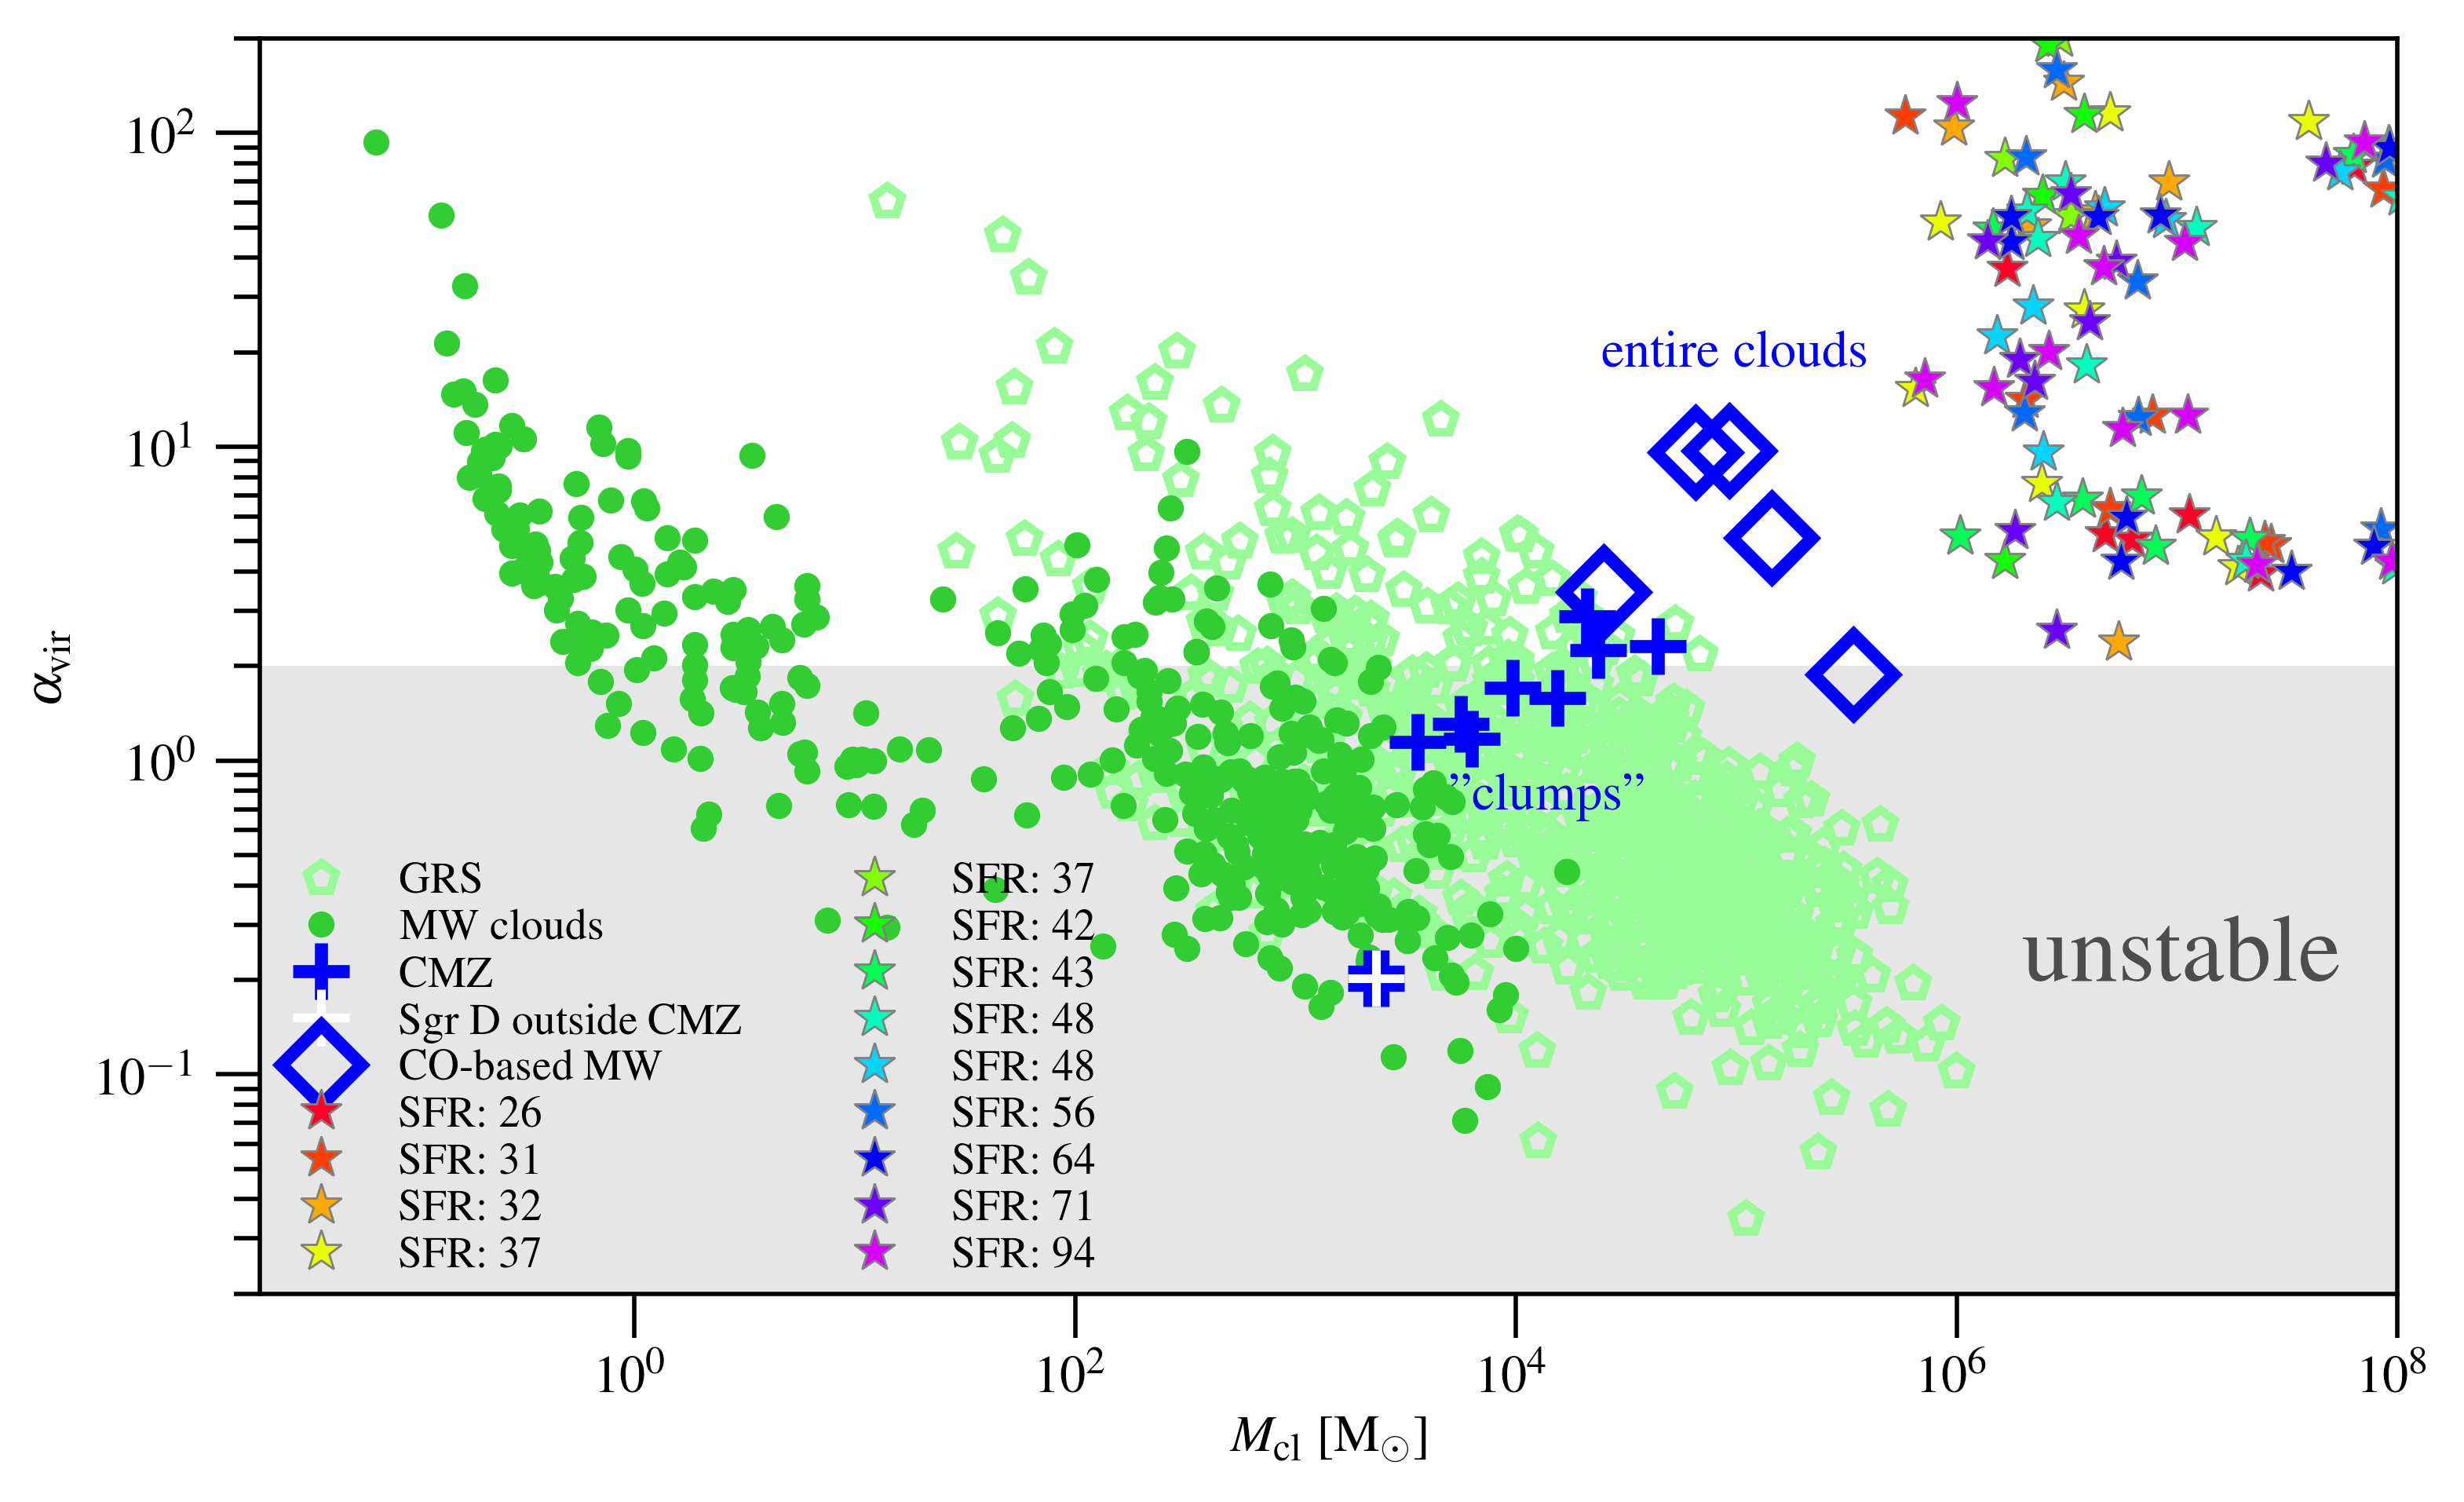
\includegraphics[trim=5 5 8 8, clip, width=0.515\textwidth]{\figpath/ss16-28_alphavir.png}
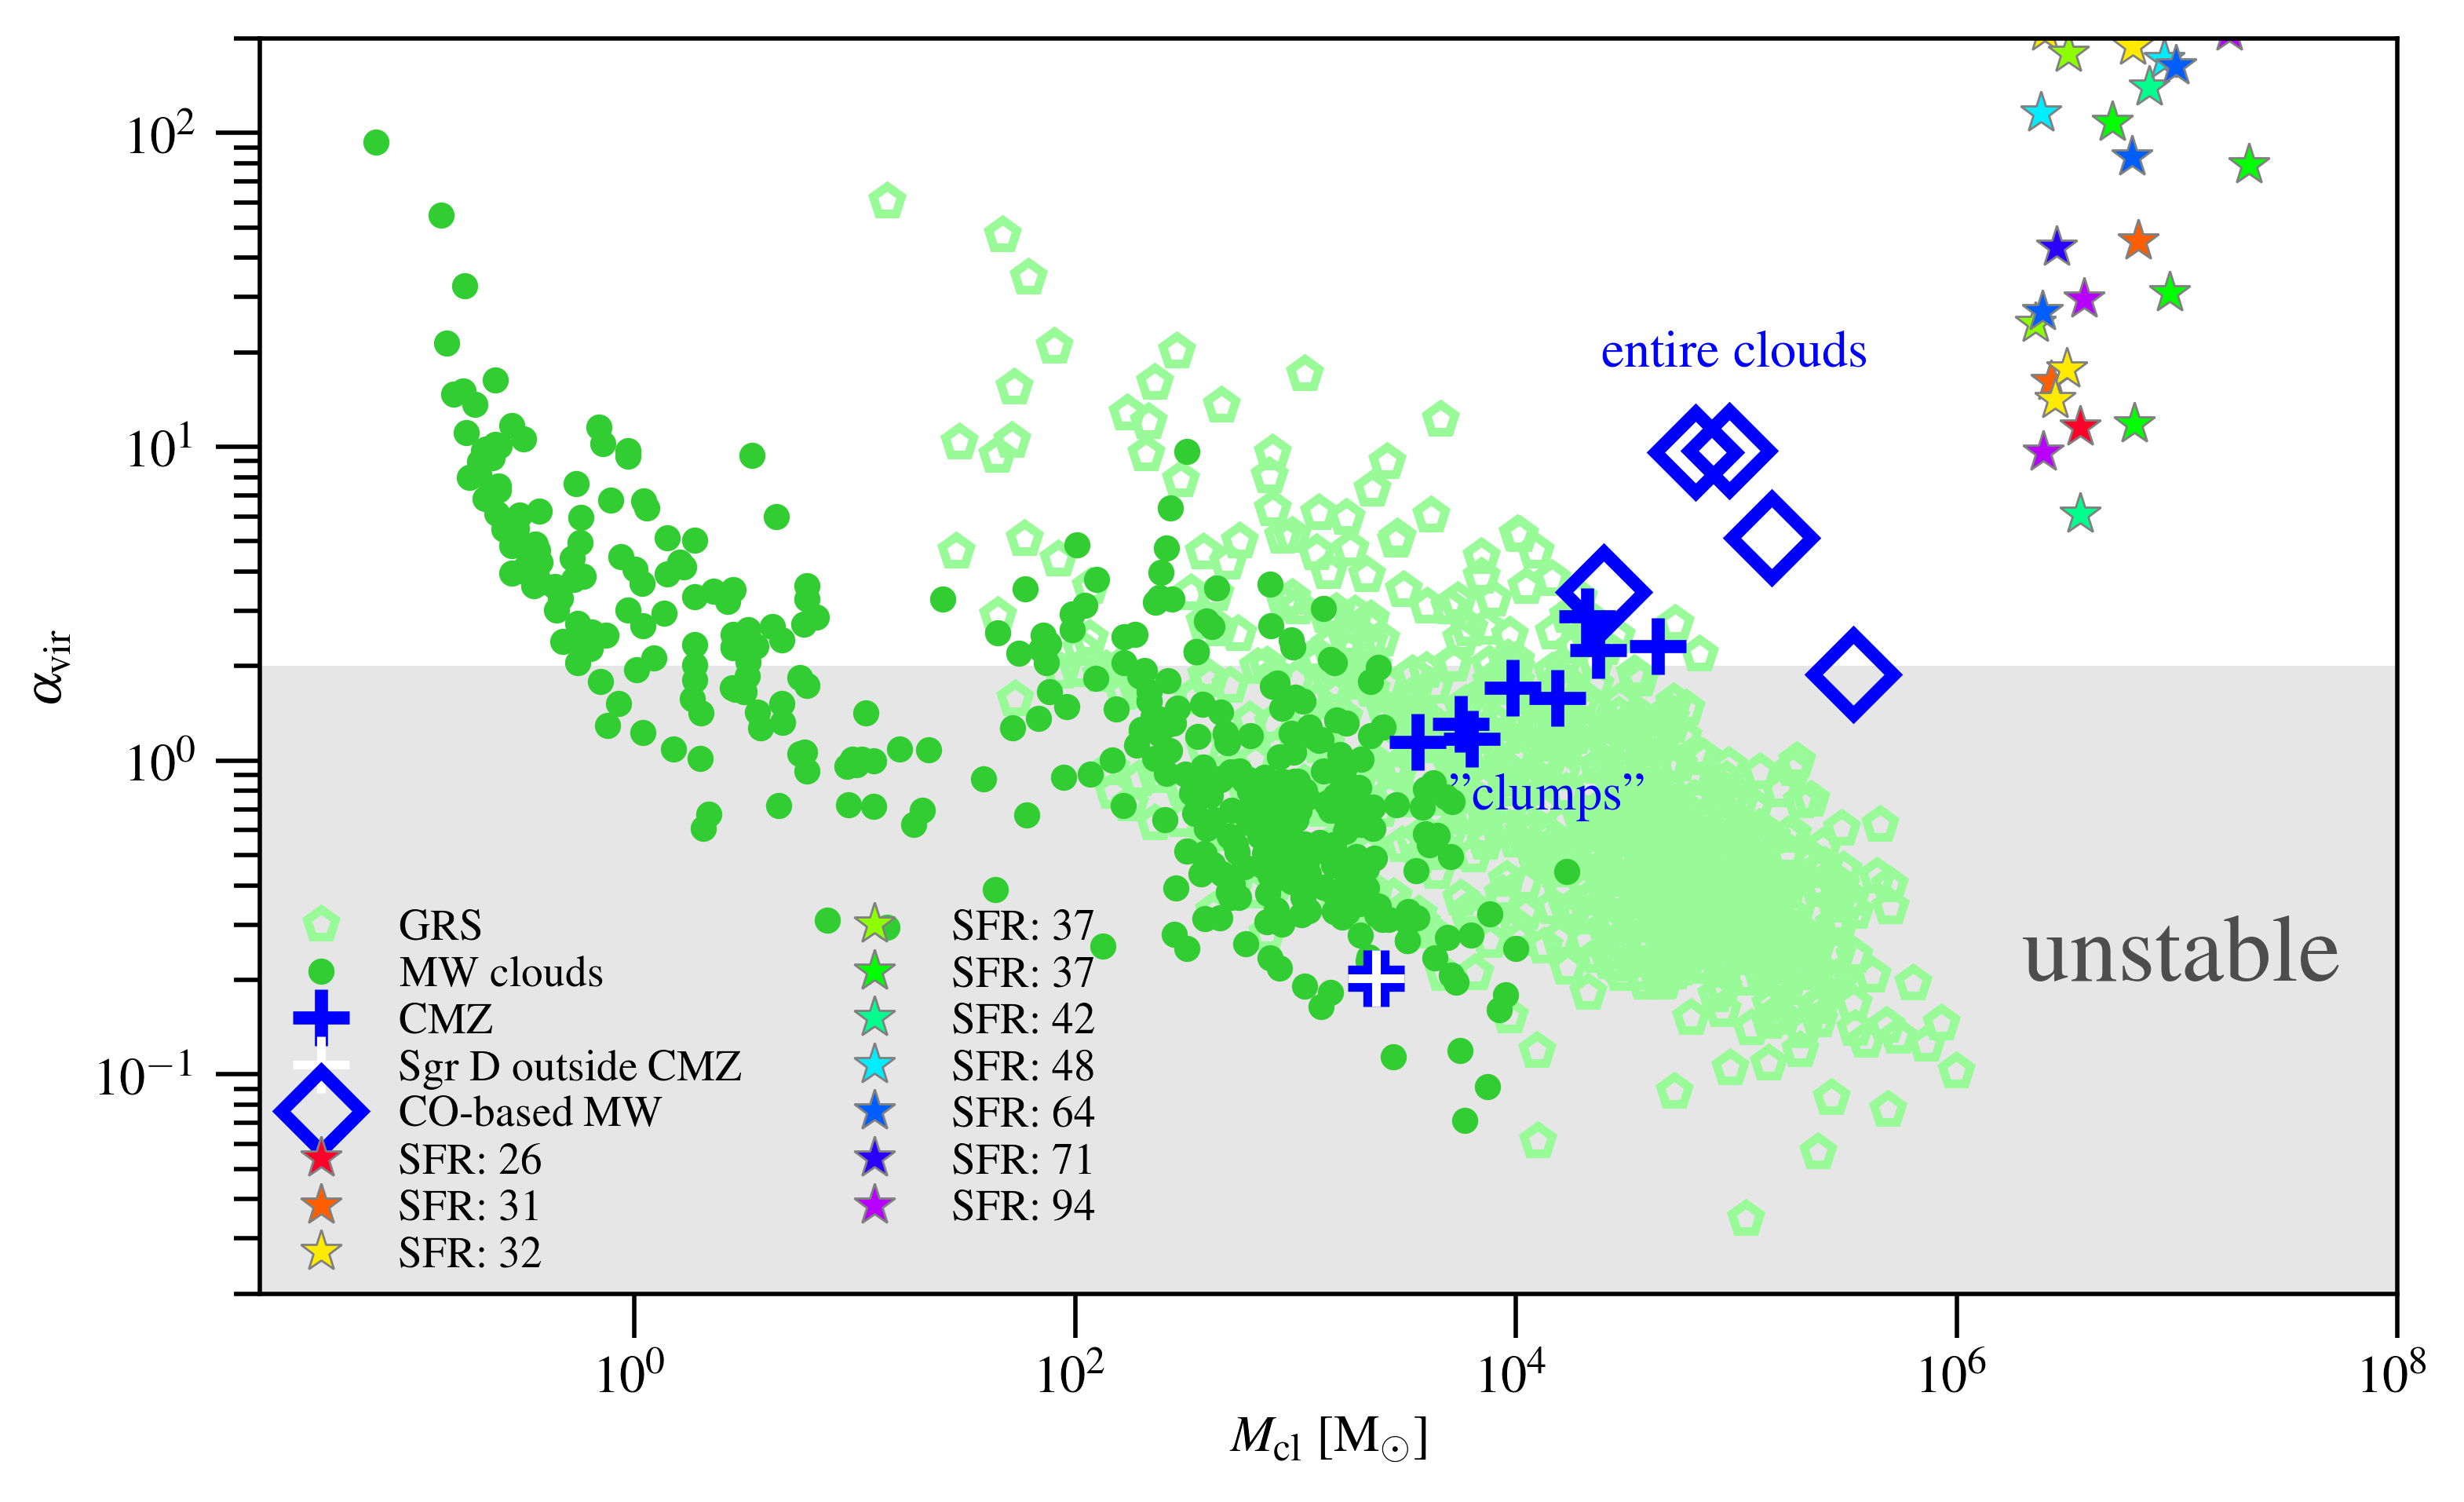
\includegraphics[trim=50 5 5 6, clip, width=0.472\textwidth]{\figpath/ss16-28-alphavir-highncut.png}
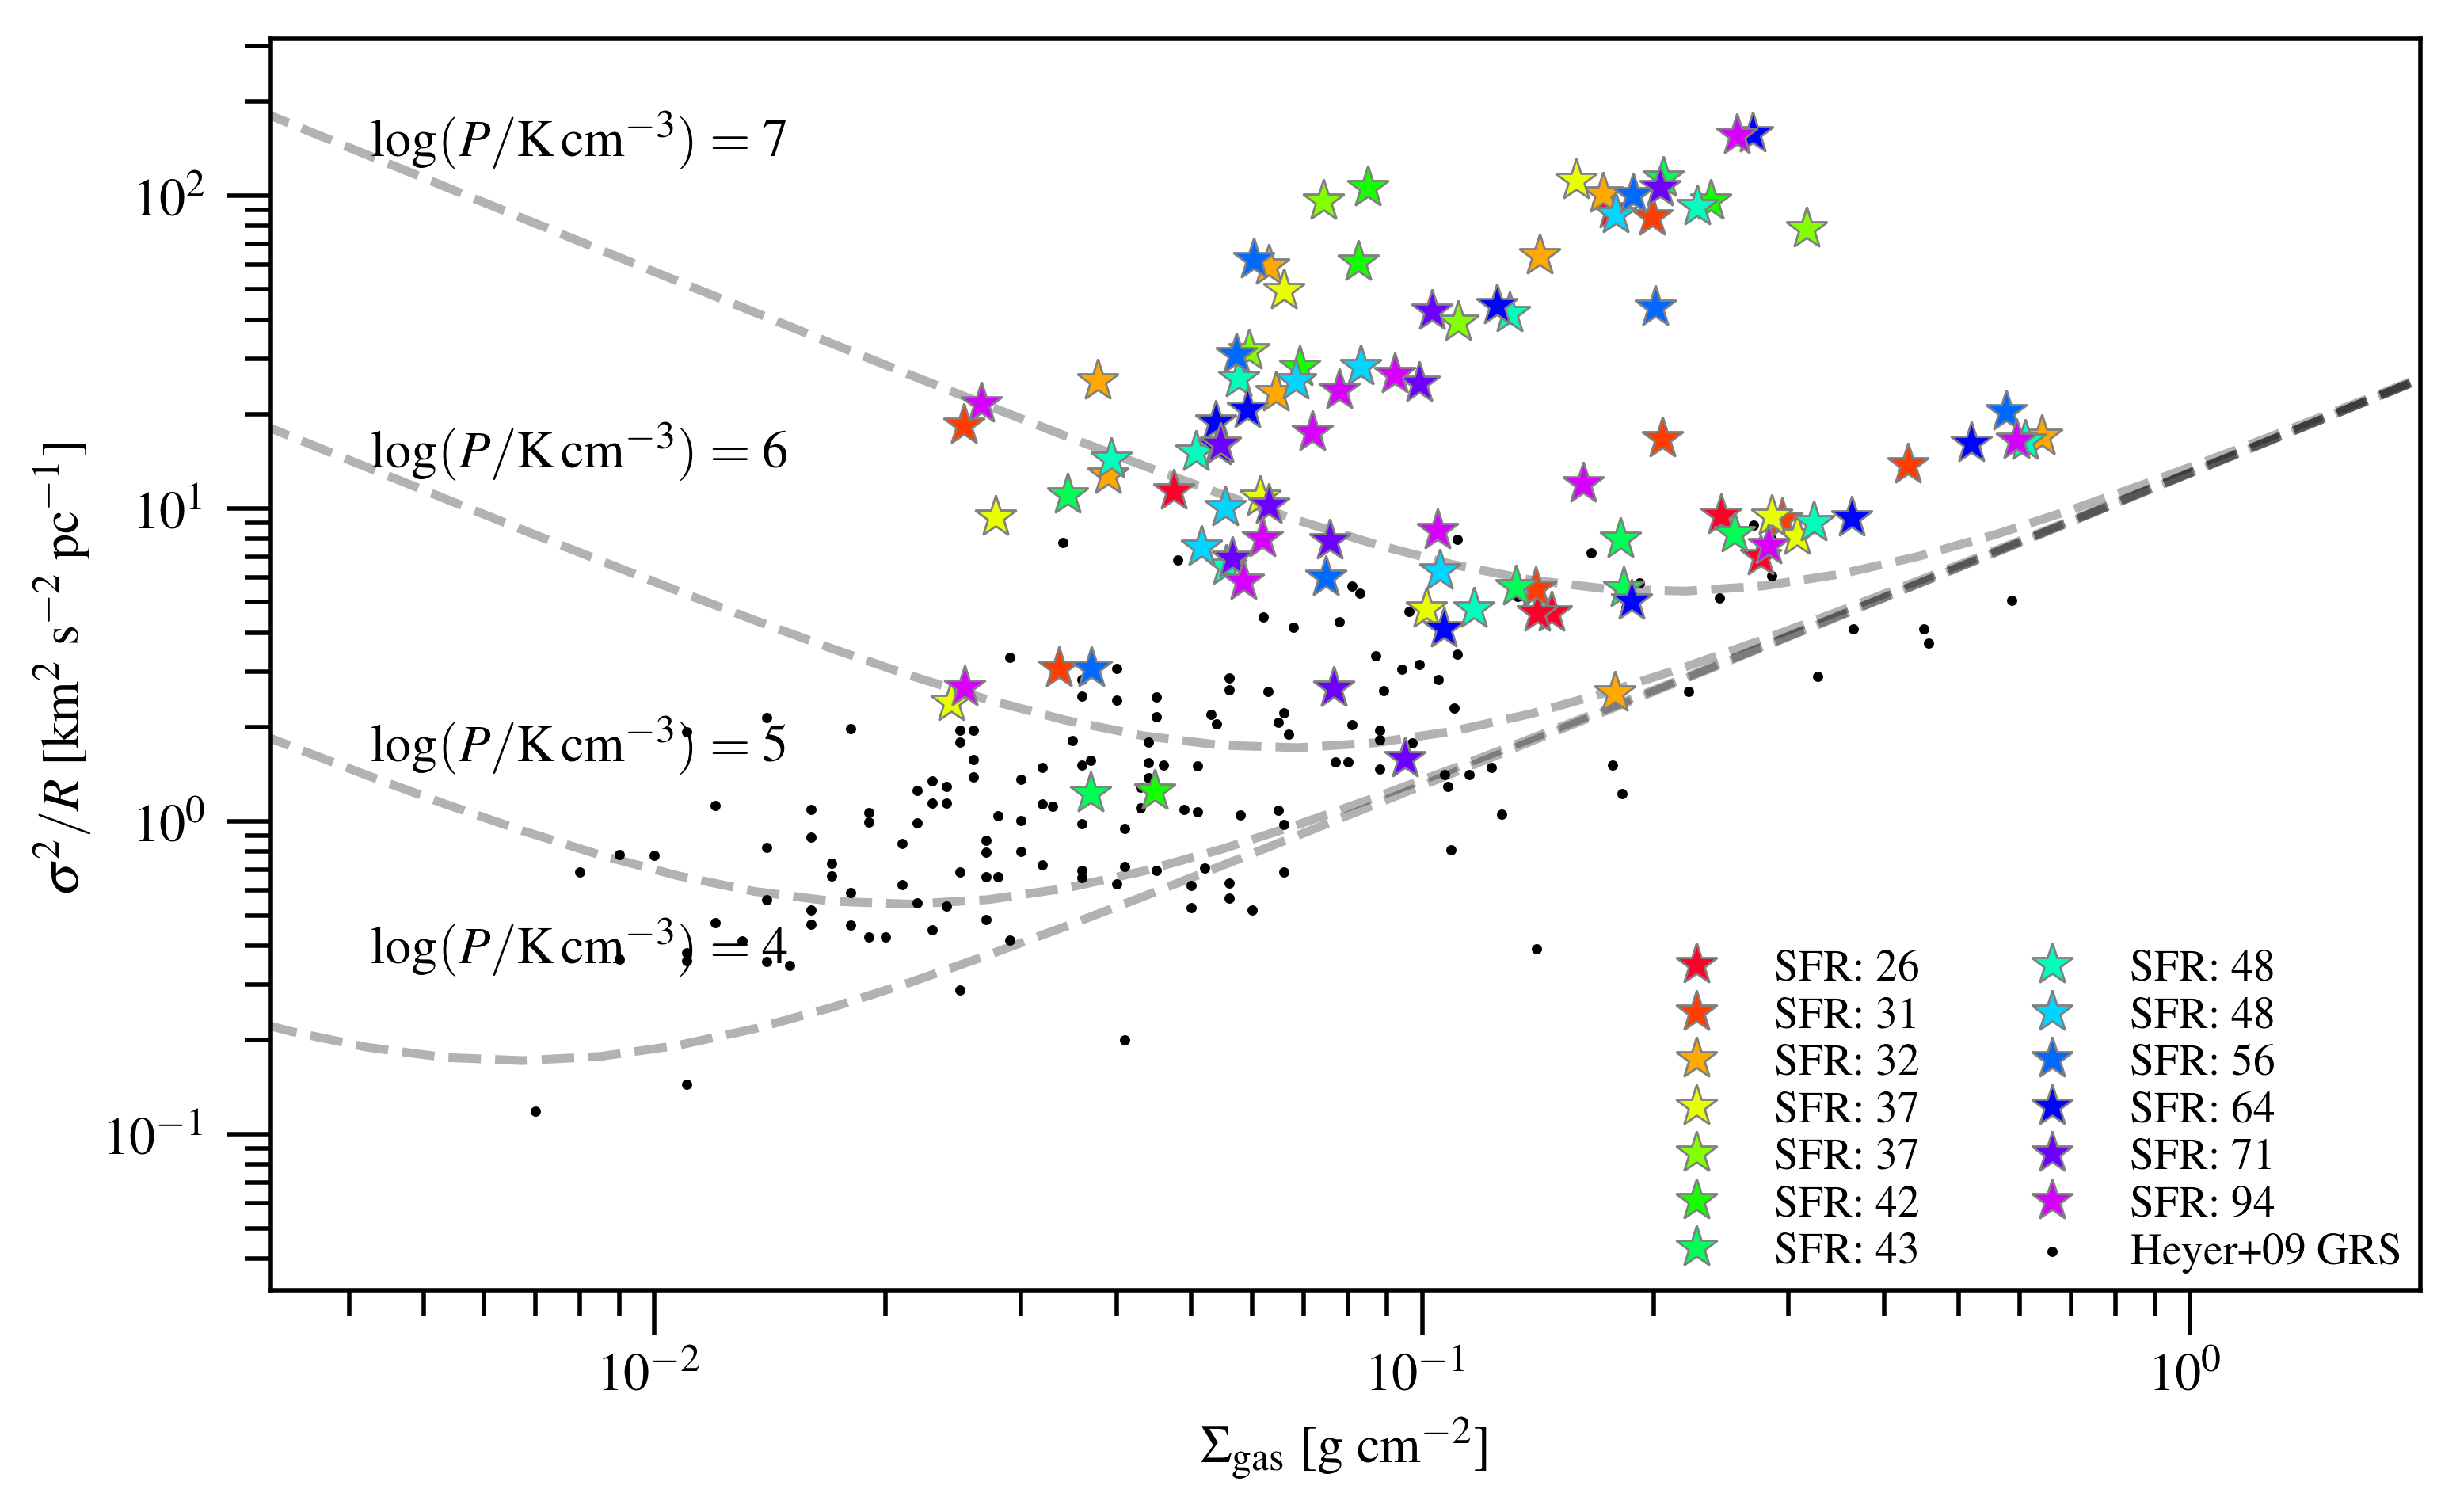
\includegraphics[trim=5 5 8 8, clip, width=0.512\textwidth]{\figpath/ss16-28_PVE.png}
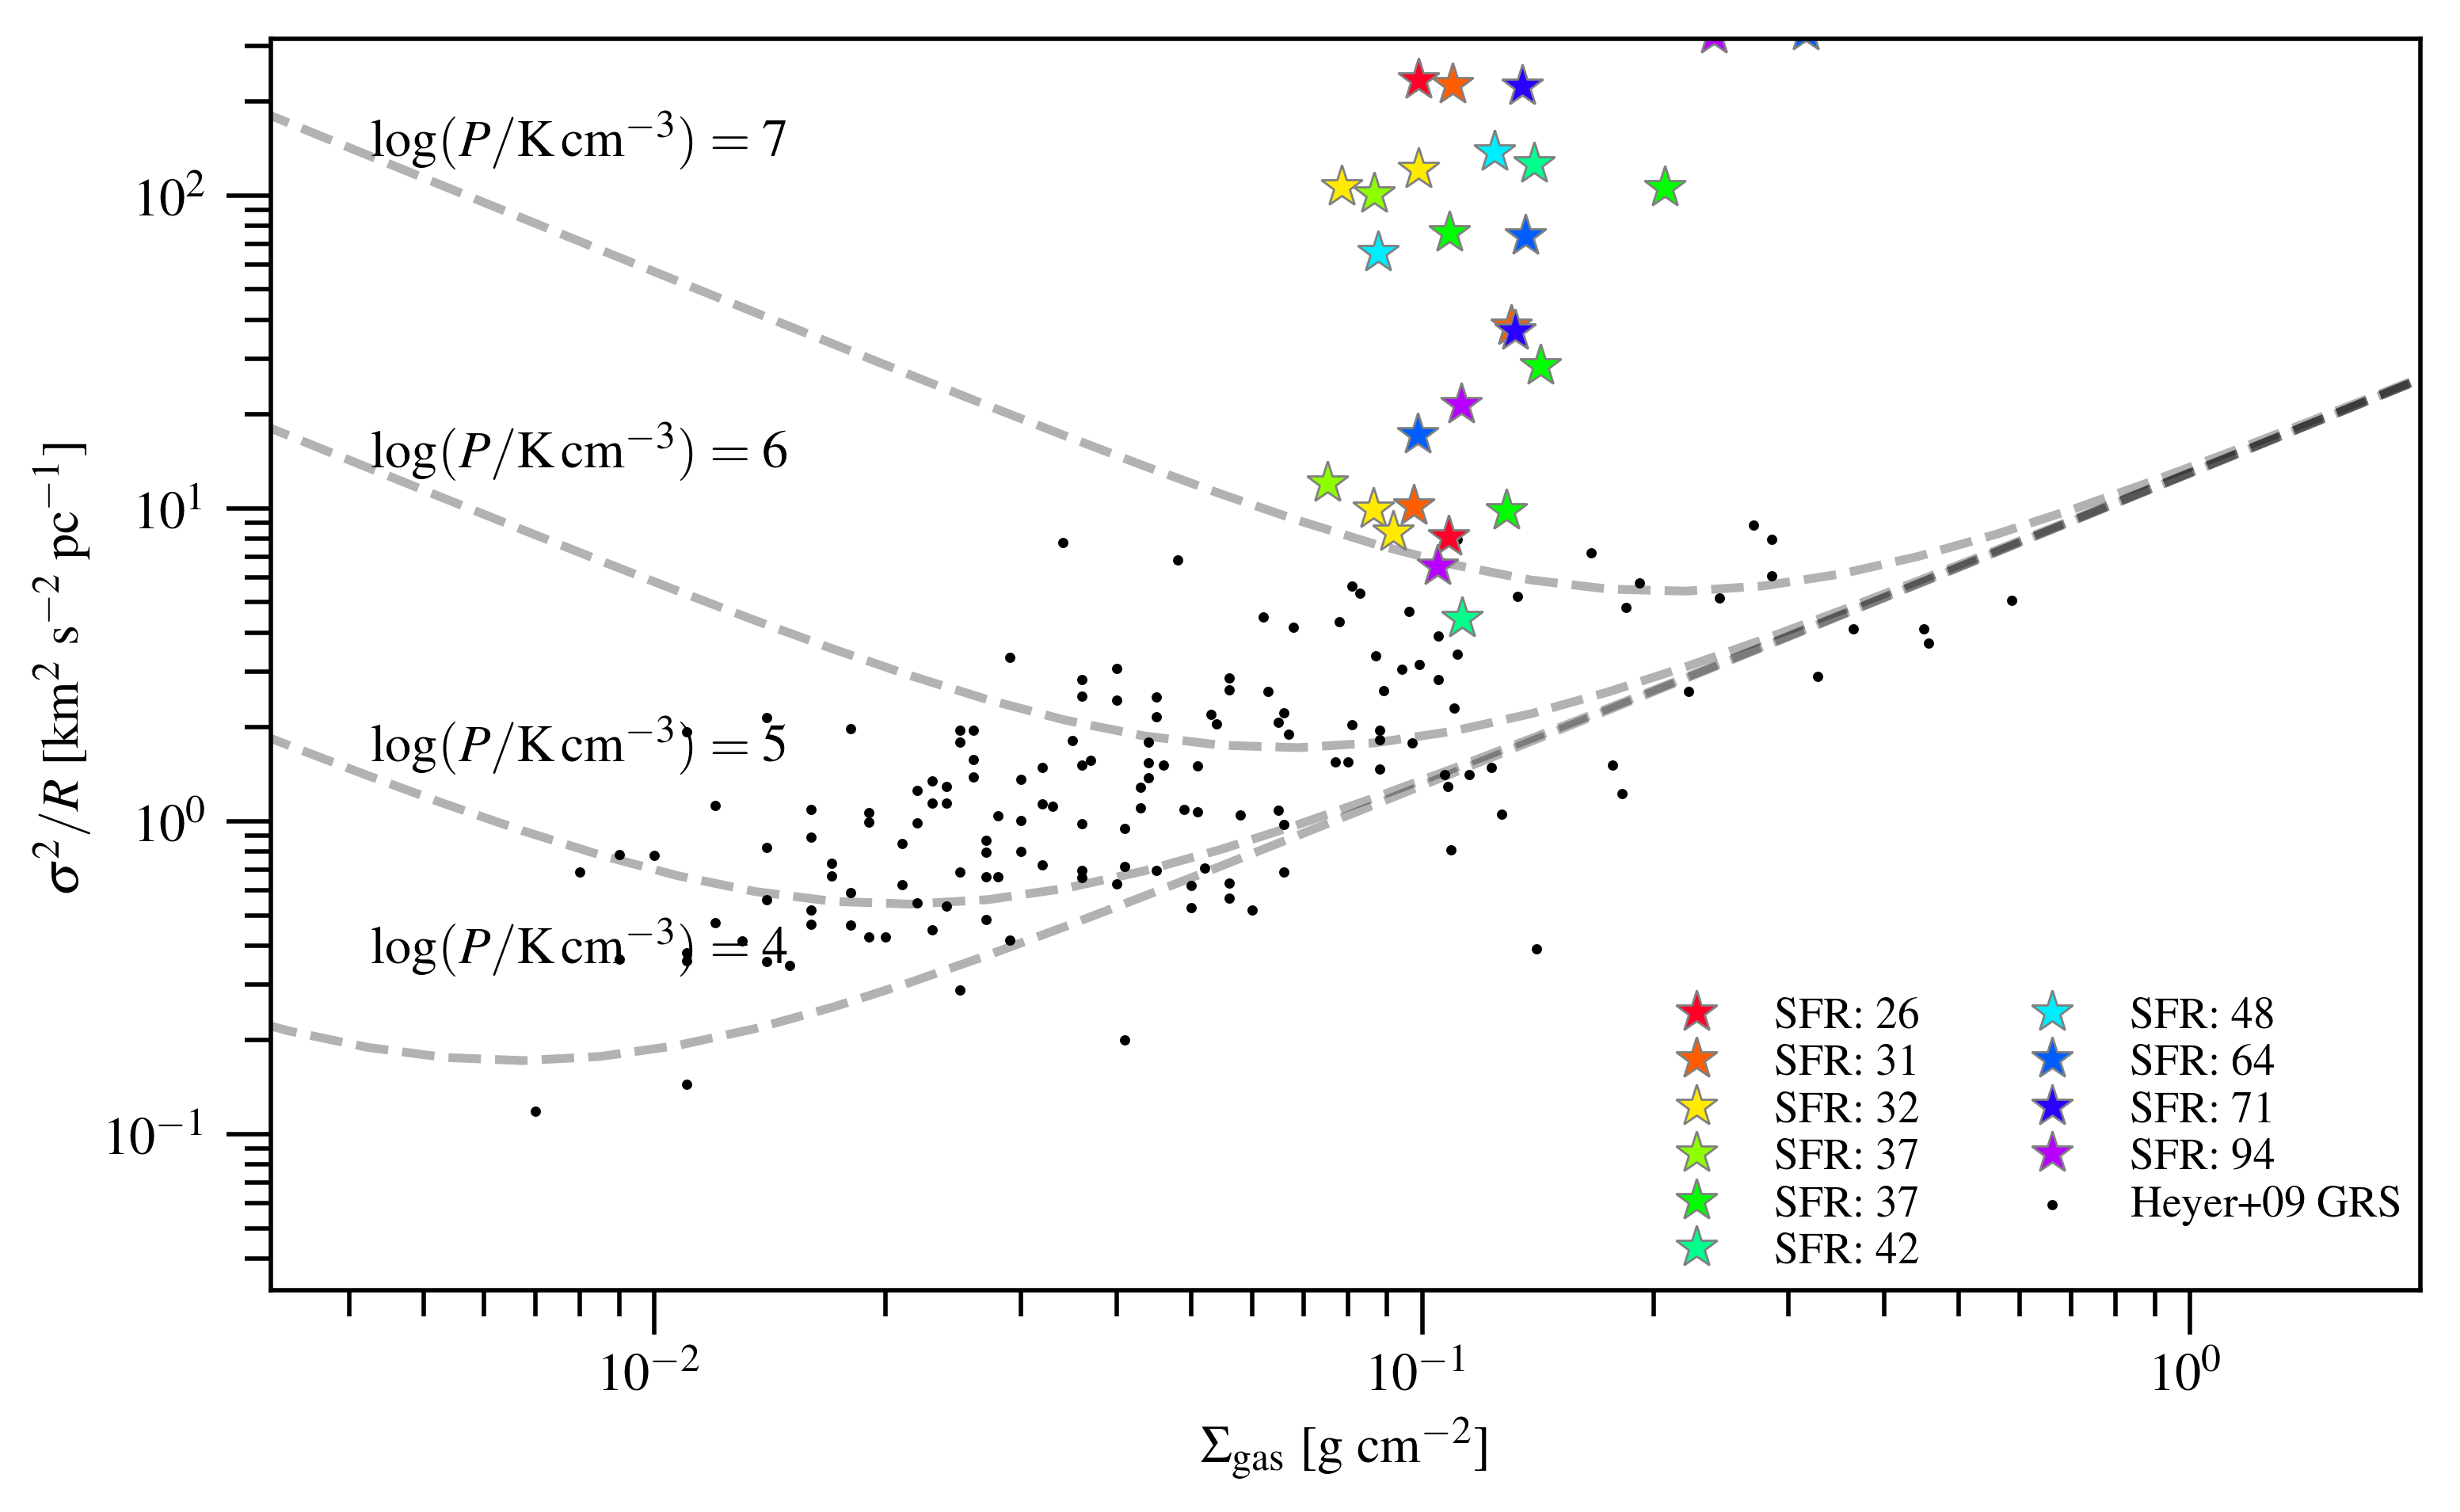
\includegraphics[trim=50 5 5 6, clip, width=0.472\textwidth]{\figpath/ss16-28-PVE-highncut.png}
\caption{
Same as \Fig{alpha16} (top panels) and \Fig{alpha27} (bottom panels), but for MCCs identified across all evolutionary stages
(i.e., with different SFR). Star symbols are color-coded by increasing SFR.
Right panels correspond to including only the denser substructures/sub-MCCs identified in \flower
(i.e., MCCs here are identified with the highest $n_{\rm cut}$, see \Sec{method}).
We find no obvious differences in relation to those observed in nearby and \highz
galaxies in the context of these cloud scaling relations.
\label{fig:alpha16-28}}
\end{figure*}
\end{comment}

\end{document}
